\vspace{0.015\textheight}
We present results in the \phojets data with and without the \met$>20$~\etUnits requirement. In the \phoonejet and \photwojet event samples, we measure the \et of the photon, the \et of the leading jet, $H_{T}$ (scalar sum of all EM objects, jets and \met), \met, and the invariant mass of the photon and leading jet. In addition, in the \photwojet sample, we measure the invariant mass of the photon and the two leading jets and the invariant mass of the two leading jets.

Figures \ref{fig:pjSetOne}--\ref{fig:pjSetFour} show Method A results without the \met requirement, and Figures \ref{fig:pjMetSetOne}--\ref{fig:pjMetSetFour} show Method A results with the \met requirement. The data are represented by black circles, and the backgrounds are shown in different colors. As described in Chapter~\ref{chp:Backgrounds}, the SM backgrounds include prompt $\gamma$ production (labeled \newterm{$\gamma$ MC}), QCD multijet production (labeled \newterm{QCD}), prompt diphoton production (labeled \newterm{Di-$\gamma$}), and electroweak production (labeled \newterm{EWK}). The non-collision backgrounds from cosmic rays and the beam halo are labeled \newterm{Non-collision}. The top plot uses a logarithmic scale. The shaded region indicates the total systematic uncertainty ($\pm1\sigma$), which includes the statistical uncertainty on the total background prediction.

The uncertainty due to the jet energy scale is by far the largest systematic uncertainty. Other sources of uncertainty that are taken into account include the following: parton density functions (PDFs), initial and final state radiation (ISR/FSR), dependence on the renormalization, factorization and fragmentation scales ($Q^{2}$), the strong coupling constant ($\alpha_{s}$), the fake photon fraction determination, integrated luminosity, EM energy measurements, the beam halo estimate, and the cosmic ray background estimate.

Tables~\ref{tab:bgsummary_gjet} and \ref{tab:bgsummary_gjetmet} describe the total number of data events selected and the expected number of background events for the samples being studied. The dominant backgrounds, SM $\gamma$ and QCD multijet, are significantly reduced with the \met requirement.

%%%%%%%%%%%%%%%%%%%% Background Summary for g+jets sample %%%%%%%%%%%%%
\begin{table}[p]
\caption{Summary of background estimates for the \phoonejet and \photwojet data samples evaluated by \mbox{Method A}. Where two uncertainties are quoted, the first is statistical and the second is systematic.}
\label{tab:bgsummary_gjet}
\centering
\begin{tabular} {lcc}
%\hline
\BUbf{Background} & \BUbf{\boldmath$\gamma$ + $\geq$1 Jet Sample} & \BUbf{\boldmath$\gamma$ + $\geq$2 Jet Sample} \\
\hline
Prompt $\gamma$ & 3387044 $\pm$ 1840 $\pm$ 108938& 629569 $\pm$ 793 $\pm$
39721\\
QCD & 1472467 $\pm$ 1213 $\pm$ 27108 & 273681 $\pm$ 523 $\pm$
6095 \\
Electroweak & 11765 $\pm$ 108 $\pm$ 952& 1833 $\pm$ 42 $\pm$
271 \\
Diphoton & 12136 $\pm$ 110 $\pm$ 641 & 1775 $\pm$ 42 $\pm$
196 \\
Non-Collision & 132 $\pm$ 11 $\pm$ 4 & 8 $\pm$ 2 $\pm$ 1 \\
\hline
\BUbf{\phojets Data} & 4883544 $\pm$ 2209 & 906866 $\pm$ 952\\
\hline
\end{tabular}
\end{table}

%%%%%%%%%%%%%%%%%%%% Background Summary for g+jets+MET>20 sample %%%%%%%%%%%%%
\begin{table}[p]
\caption{Summary of background estimates for the \phoonejet + \met$>$~20 \etUnits and \photwojet + \met$>$~20 \etUnits data samples evaluated by \mbox{Method A}. Where two uncertainties are quoted, the first is statistical and the second is systematic.}
\label{tab:bgsummary_gjetmet}
\centering
\begin{tabular} {lcc}
%\hline
\BUbf{Background} & \BUbf{\boldmath$\gamma$ + $\geq$1 Jet} & \BUbf{\boldmath$\gamma$ + $\geq$2 Jet} \\
 & \BUbf{+ \met$>$~20 \etUnits Sample} & \BUbf{+ \met$>$~20 \etUnits Sample} \\
\hline
Prompt $\gamma$ & 88878 $\pm$ 366 $\pm$ 3178 & 28502 $\pm$ 168 $\pm$ 1429 \\
QCD & 38527 $\pm$ 196 $\pm$ 1664 & 12385 $\pm$ 111 $\pm$
524 \\
Electroweak & 6271 $\pm$ 79 $\pm$ 613 & 843 $\pm$ 29 $\pm$
122 \\
Diphoton & 355 $\pm$ 19 $\pm$ 13 & 86 $\pm$ 9 $\pm$
8 \\
Non-Collision & 124 $\pm$ 12 $\pm$ 4 & 8 $\pm$ 3 $\pm$ 1 \\
\hline
\BUbf{\phojets Data} & 134155 $\pm$ 366 & 41824 $\pm$ 204\\
\hline
\end{tabular}
\end{table}

\section{Photon \et Measurement}
We have measured the photon \et spectrum from 30 \etUnits to about 550 \etUnits, and over this range the total systematic uncertainty increases from 15\% to 90\%. It is evident that the photon purity increases at higher \et. The photon \et is one of the strongest measurements sensitive to any excess production over the SM prediction of photon + jets events. Our measurement from Method A agrees perfectly with the SM expectation. Furthermore, this confirms the accuracy of the background modeling and calculated expectation over the complete photon \et range. The statistics are limited at high-\et.

\section{Leading Jet \et Measurement}
The leading jet \et measurement has similar implications to that of the photon \et. The hump (or \newterm{turn-on}) seen in the lower \et region is due to the asymmetric requirement on the minimum jet \et. At leading order, the leading jet should balance the photon which has \etg{30}. As measured by Method A, the \pythiaText LO calculation seems to produce the jet \et spectrum reasonably well. The dip seen in the ratio plot (for \textit{e.g.} jet \et in Fig.~\ref{fig:pjSetOne}) is due to the difference in the resolution of the control samples to that of the data. As mentioned in Section~\ref{sec:QCDbackground}, the QCD events in the photon + jets events passing tight photon selection requirements are often from quark jets faking photons. But the control samples, like the sideband events we used to model QCD events, are mostly gluon jets passing loose photon selection requirements. These gluon jets tend to have a relatively large amount of energy in the isolation cone (outside the photon cluster but inside the clustering cone), which is not added to the sideband photon candidate. The largest systematic uncertainty for the measurement is the JES.

\section{Mass Measurements}
The invariant mass measurement of the $\gamma$ + leading jet extends up to 1000 \massunits. Many background predictions become limited by statistics in the high mass region, and the systematic uncertainty increases from 15\% to 90\%. It is evident from these measurements that the SM $\gamma$ and QCD multijet backgrounds are dominant. However with the requirement of large \met in the event, these backgrounds are reduced and real \met from the electroweak processes ({\it e.g.} $W \to \ell \nu$) becomes significant. This \met requirement significantly improves the sensitivity to events in which a weakly interacting particle is produced like the $\widetilde{G}$ (in the decay of $\widetilde{\chi}^{0}_{1}\to\gamma\widetilde{G}$).

\section{Method A and Method B Comparison}
The backgrounds using Method A are well modeled and describe data reasonably well in most of the distributions. But a close inspection reveals discrepancies in certain distributions like lead jet \et, $H_{T}$, jet multiplicity, and \met. Some measurements show certain structures and discrepancies that are not within the systematic uncertainties. Most of these differences can be attributed to the limitations in the leading-order predictions of \pythiaText.

Figures \ref{fig:pjMtdBSetOne}--\ref{fig:pjMtdBSetFour} show the Method~B results without the \met requirement. Figures \ref{fig:pjmetMtdBSetOne}--\ref{fig:pjmetMtdBSetFour} show the Method~B results with the \met requirement. In these figures, \newterm{QCD (weighted)} indicates the weighted QCD background template that replaces the $\gamma$ MC and QCD templates of Method A. Using Method B, we are able describe some distributions much better compared to Method A. The photon \et distribution must agree with Method A by construction. The jet \et, $H_{T}$, jet multiplicity and \met distributions, however, show significant improvement and agree well with data. The \met distribution agrees well in the low \met region. Some distributions using Method B were not modeled well as expected. For example, the invariant mass of the photon and leading jet shows a large discrepancy, which is attributed to the fact that the QCD background events are from different processes (or Feynman diagrams).

\section{Jet Multiplicity and $H_{T}$ Measurements}
The jet multiplicity and $H_{T}$ measurements are particularly sensitive to extra particles produced. If there is a contribution from SUSY, we expect several extra jets. Hence, an excess of events with more than 2 jets and with large total energy should be evident. But again, given the fact that \pythiaText MC samples are leading order, the jet multiplicity distribution cannot be modeled accurately using Method A (for \textit{e.g.} see Fig.~\ref{fig:pjSetTwo:NJet}). This is exactly where the Method B modeling shows its strength and we do see good agreement between data and the background expectation.

\section{\met Measurement}
The \met distribution shows mixed results using the two methods. It should be noted that \met is one of the hardest, if not the hardest, distributions to model as it has many dependencies. For example, the effect of calorimeter energy mismeasurements and energy resolution, the uncertainty in choosing the primary vertex, uncertainties in the jet energy corrections, etc., all affect the final \met measurement. The \met is sensitive to the number of particles in the event, especially how jets are distributed and how the unclustered energy is distributed in the event. In data, there are a lot of soft (low energy) jets from the underlying event and multiple interactions, which are not well modeled by LO \pythiaText MC events, and this gives rise to a difference in the \met resolution for data and MC. This is clearly evident when Method A is used to model the \met. In Method B, using more data-based sideband events to model QCD seems to model the \met resolution in the low \met region correctly. But it fails to describe the high \met region where there is an excess of badly mismeasured jets. Together, the two results provide an adequate understanding of the measurement.



\clearpage
%%%%%%%%%%%%%%%%%%%%%%%%%%%%%% METHOD A: G30 JETS
\begin{figure*}[h!]
\centering
\subfigure[]
{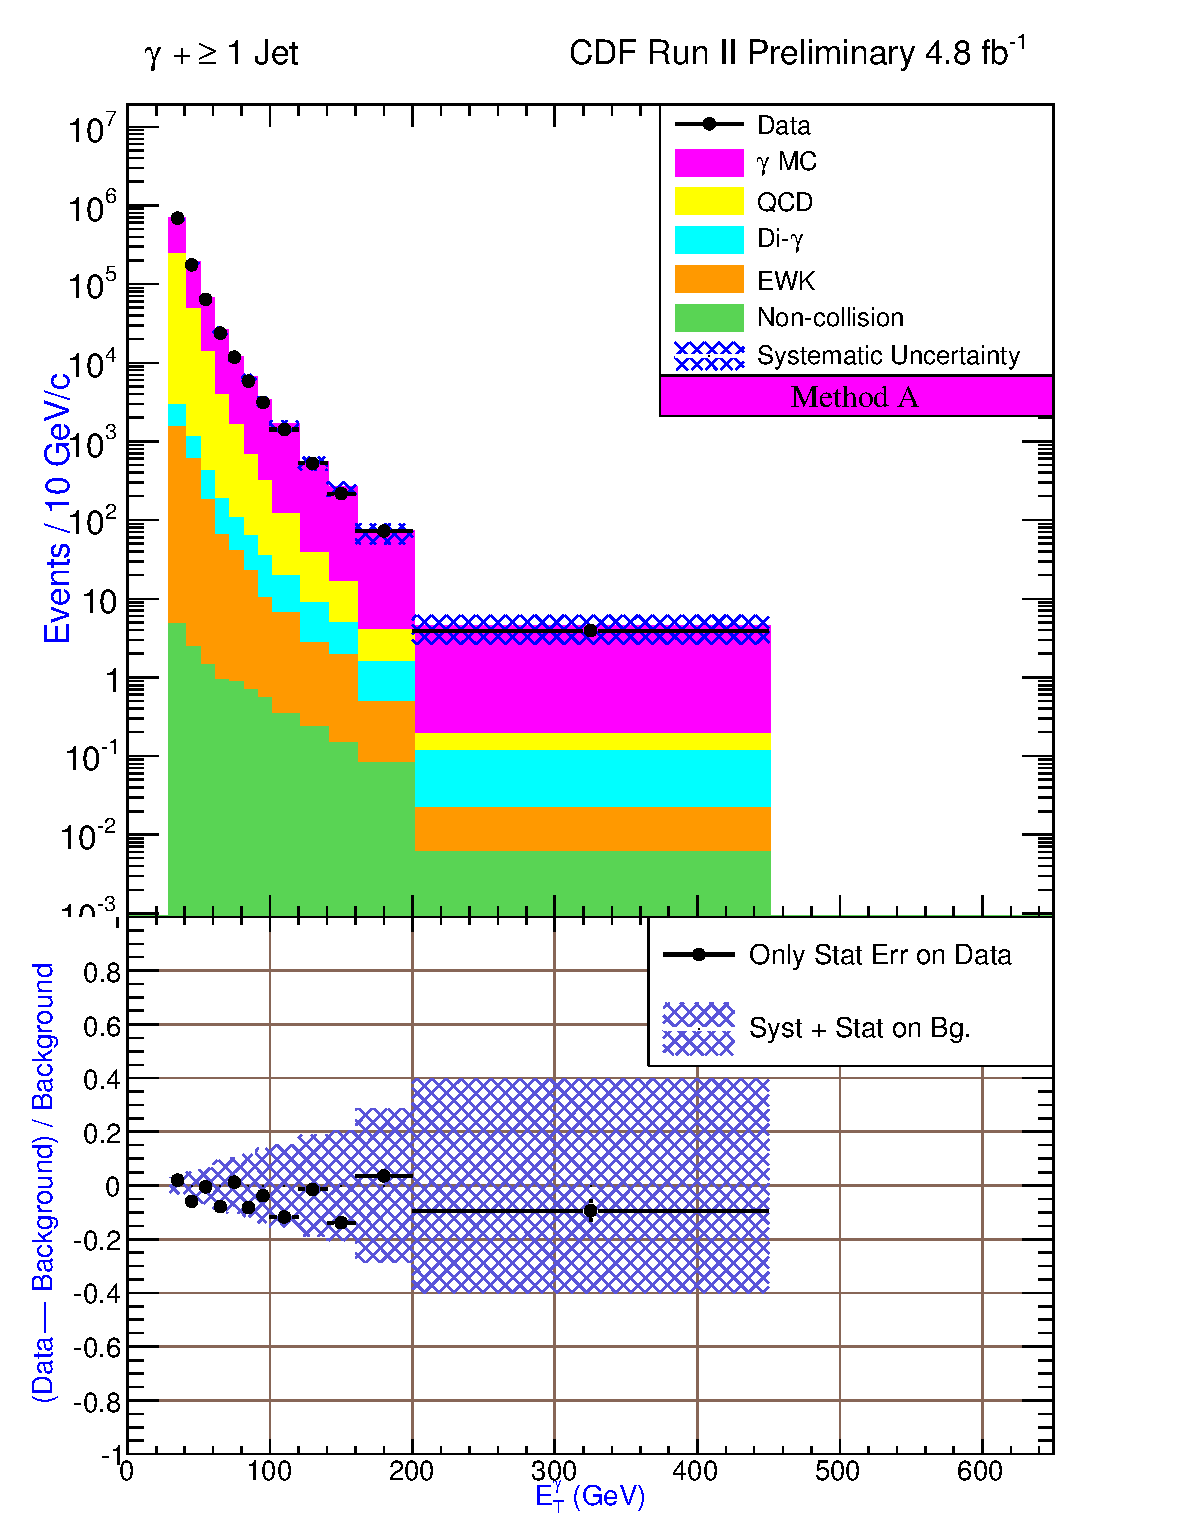
\includegraphics[keepaspectratio=true, scale=\resultsHistScale]{G30Jets_MtdA_plot1_Et_pho.pdf}}
\subfigure[]
{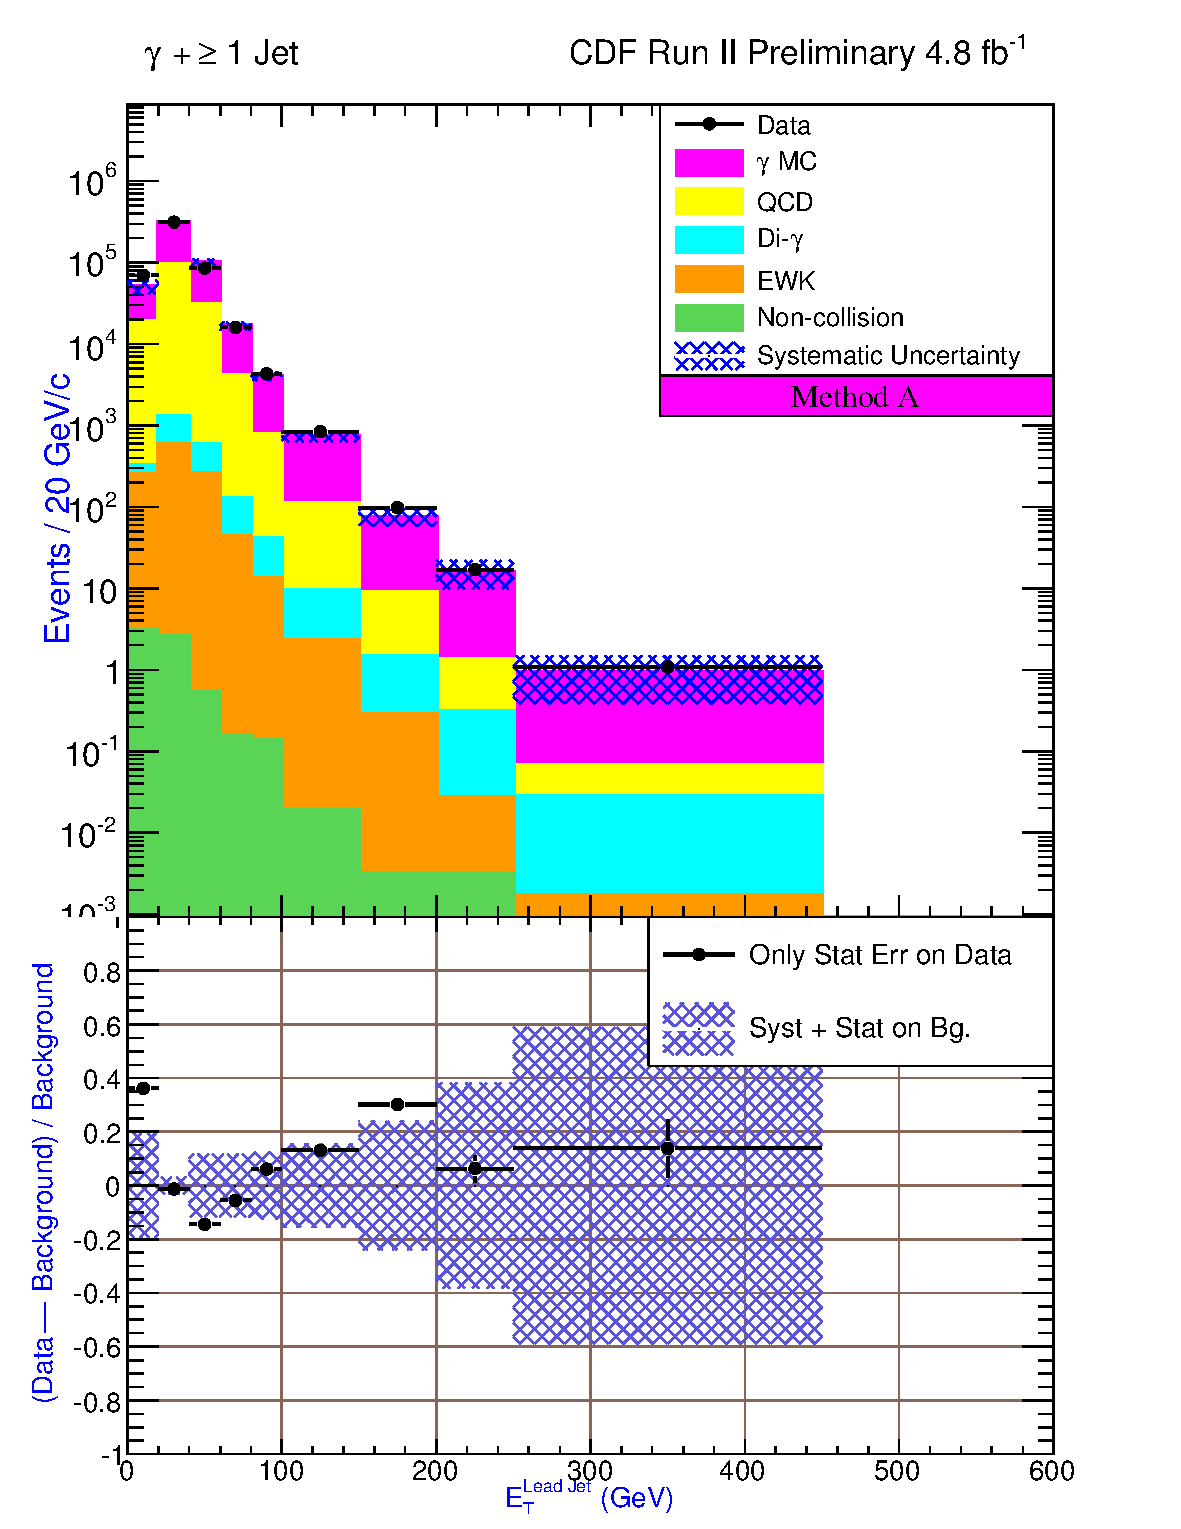
\includegraphics[keepaspectratio=true, scale=\resultsHistScale]{G30Jets_MtdA_plot1_Et_j1.pdf}
}
\subfigure[]
{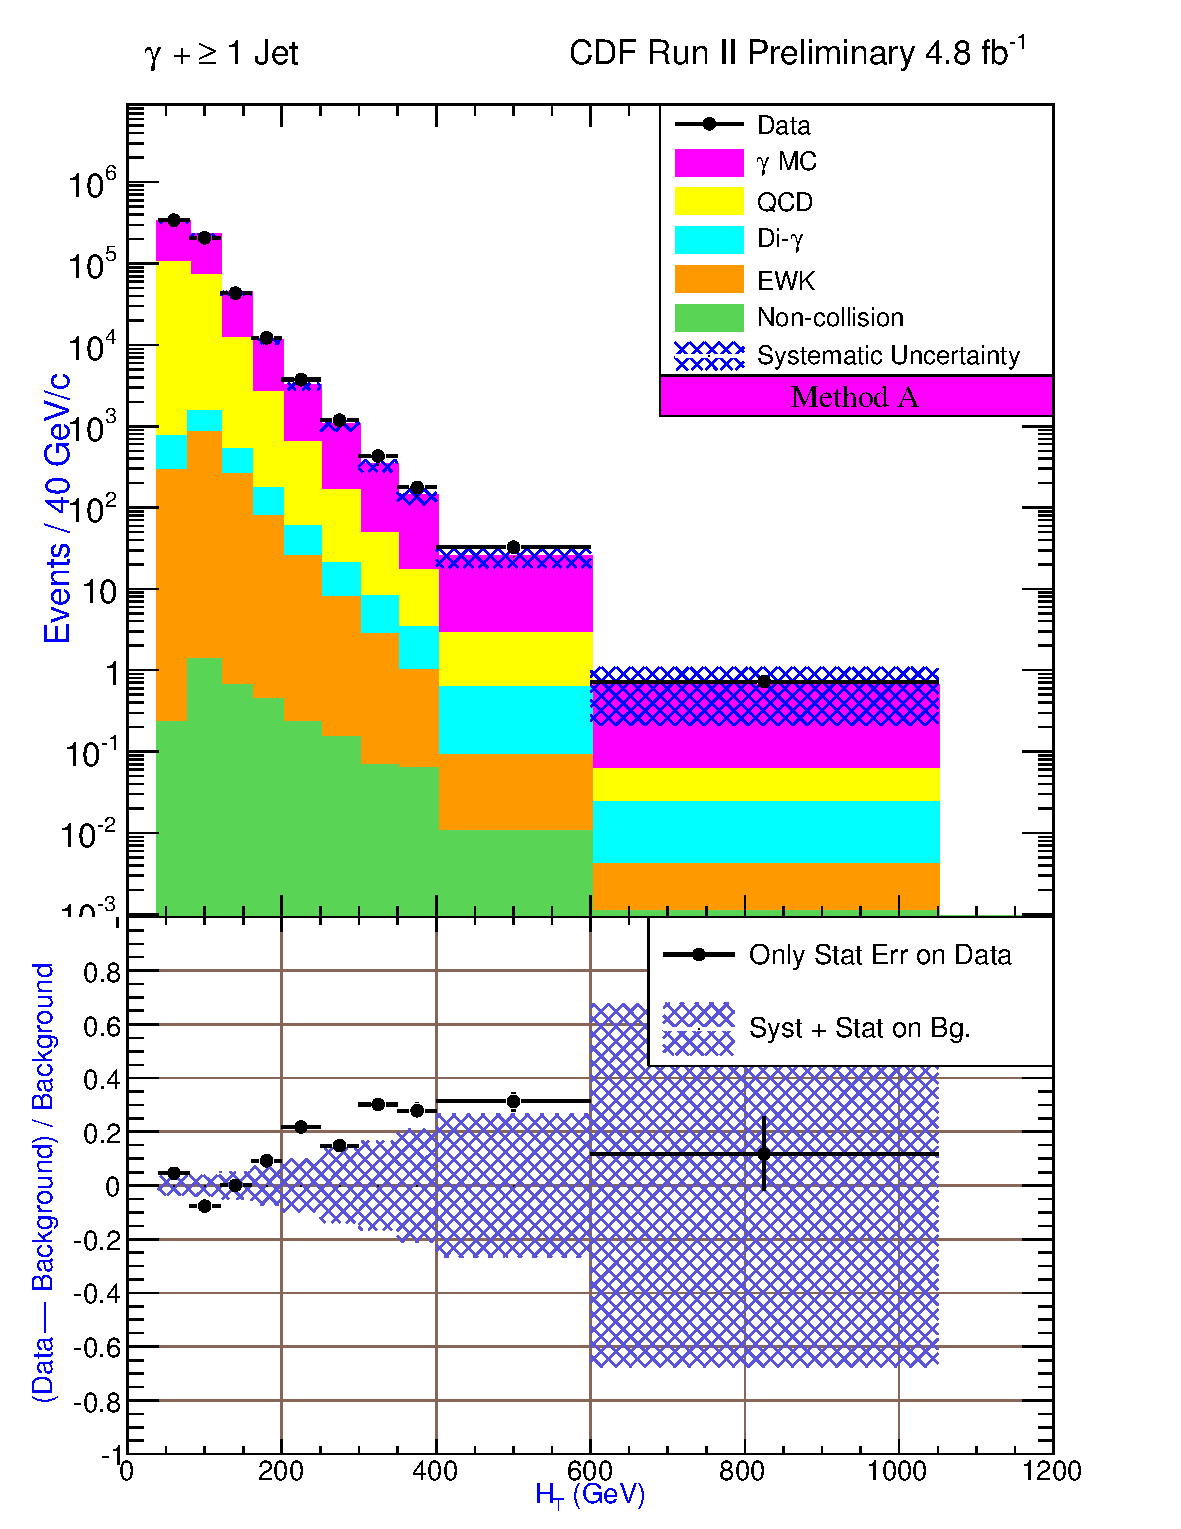
\includegraphics[keepaspectratio=true, scale=\resultsHistScale]{G30Jets_MtdA_plot1_Ht.pdf}}
\subfigure[]
{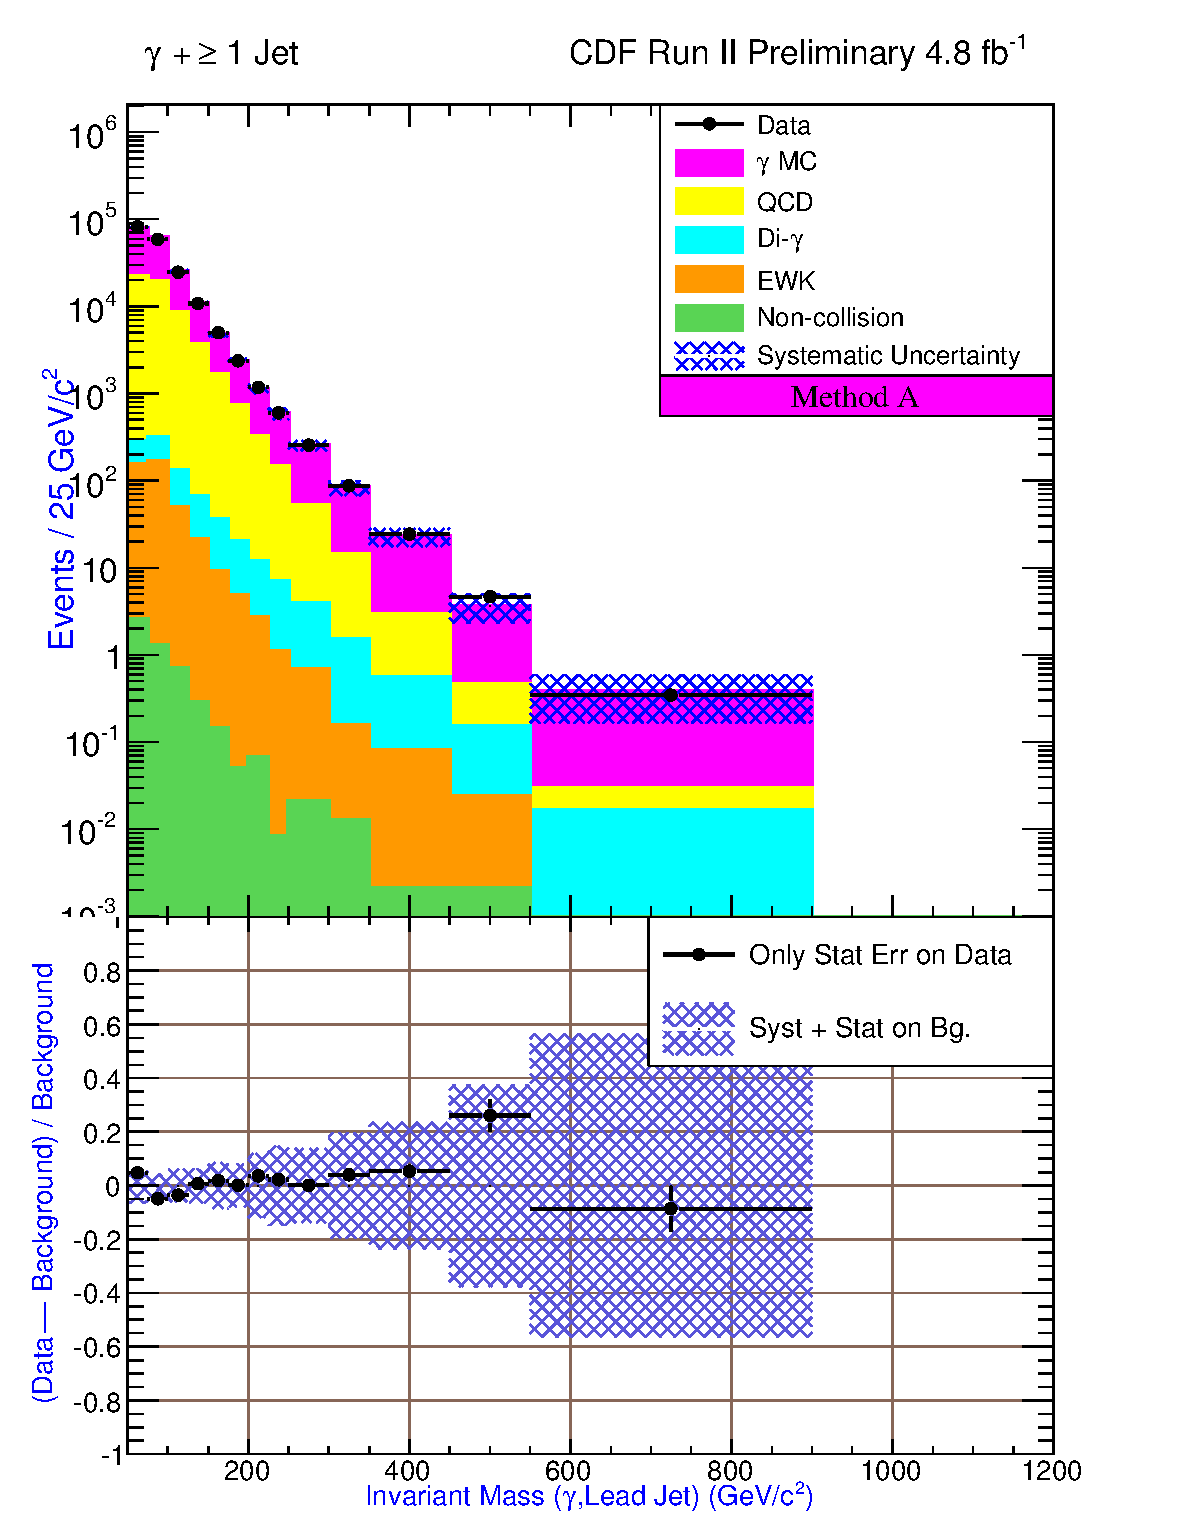
\includegraphics[keepaspectratio=true, scale=\resultsHistScale]{G30Jets_MtdA_plot1_InvMass_pj1.pdf}}
\caption{Kinematic distributions of \phoonejet events using Method A. The beginning of Chapter~\ref{chp:Results} provides a description of the elements in these distributions.}
\label{fig:pjSetOne}
\end{figure*}
\clearpage

\begin{figure*}[h!]
\centering
\subfigure[]
{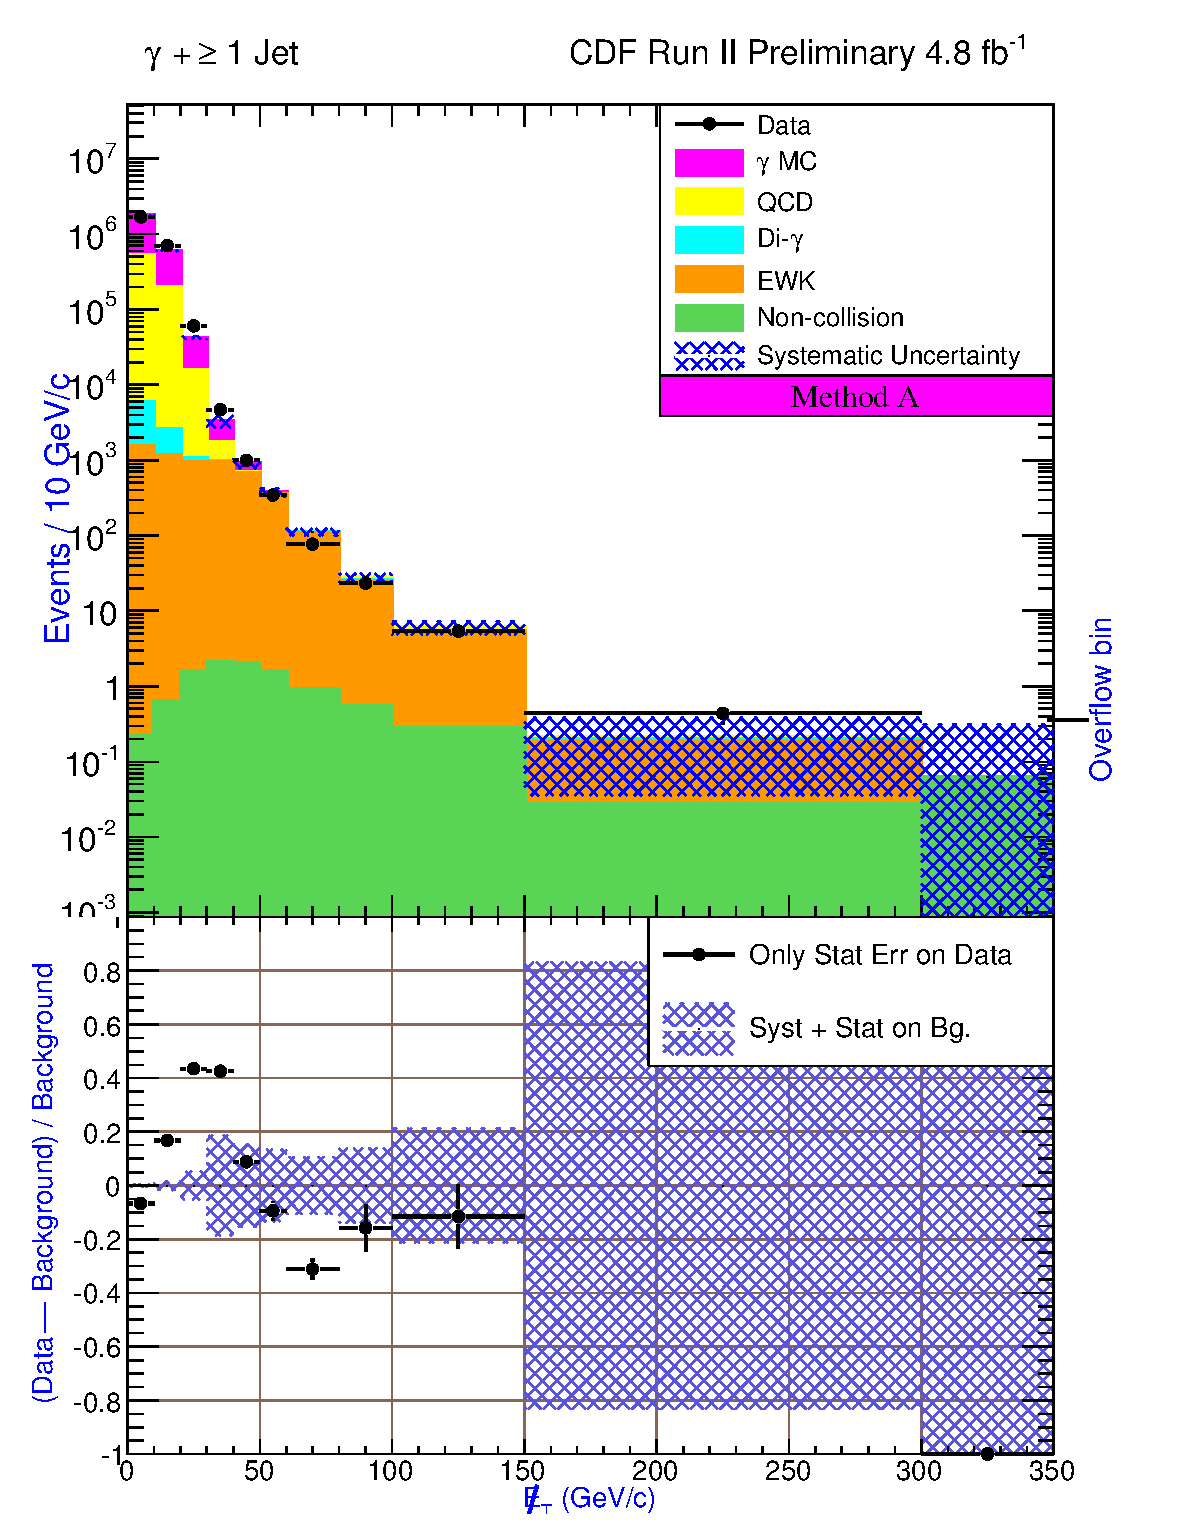
\includegraphics[keepaspectratio=true, scale=\resultsHistScale]{G30Jets_MtdA_plot1_Met.pdf}}
\subfigure[]
{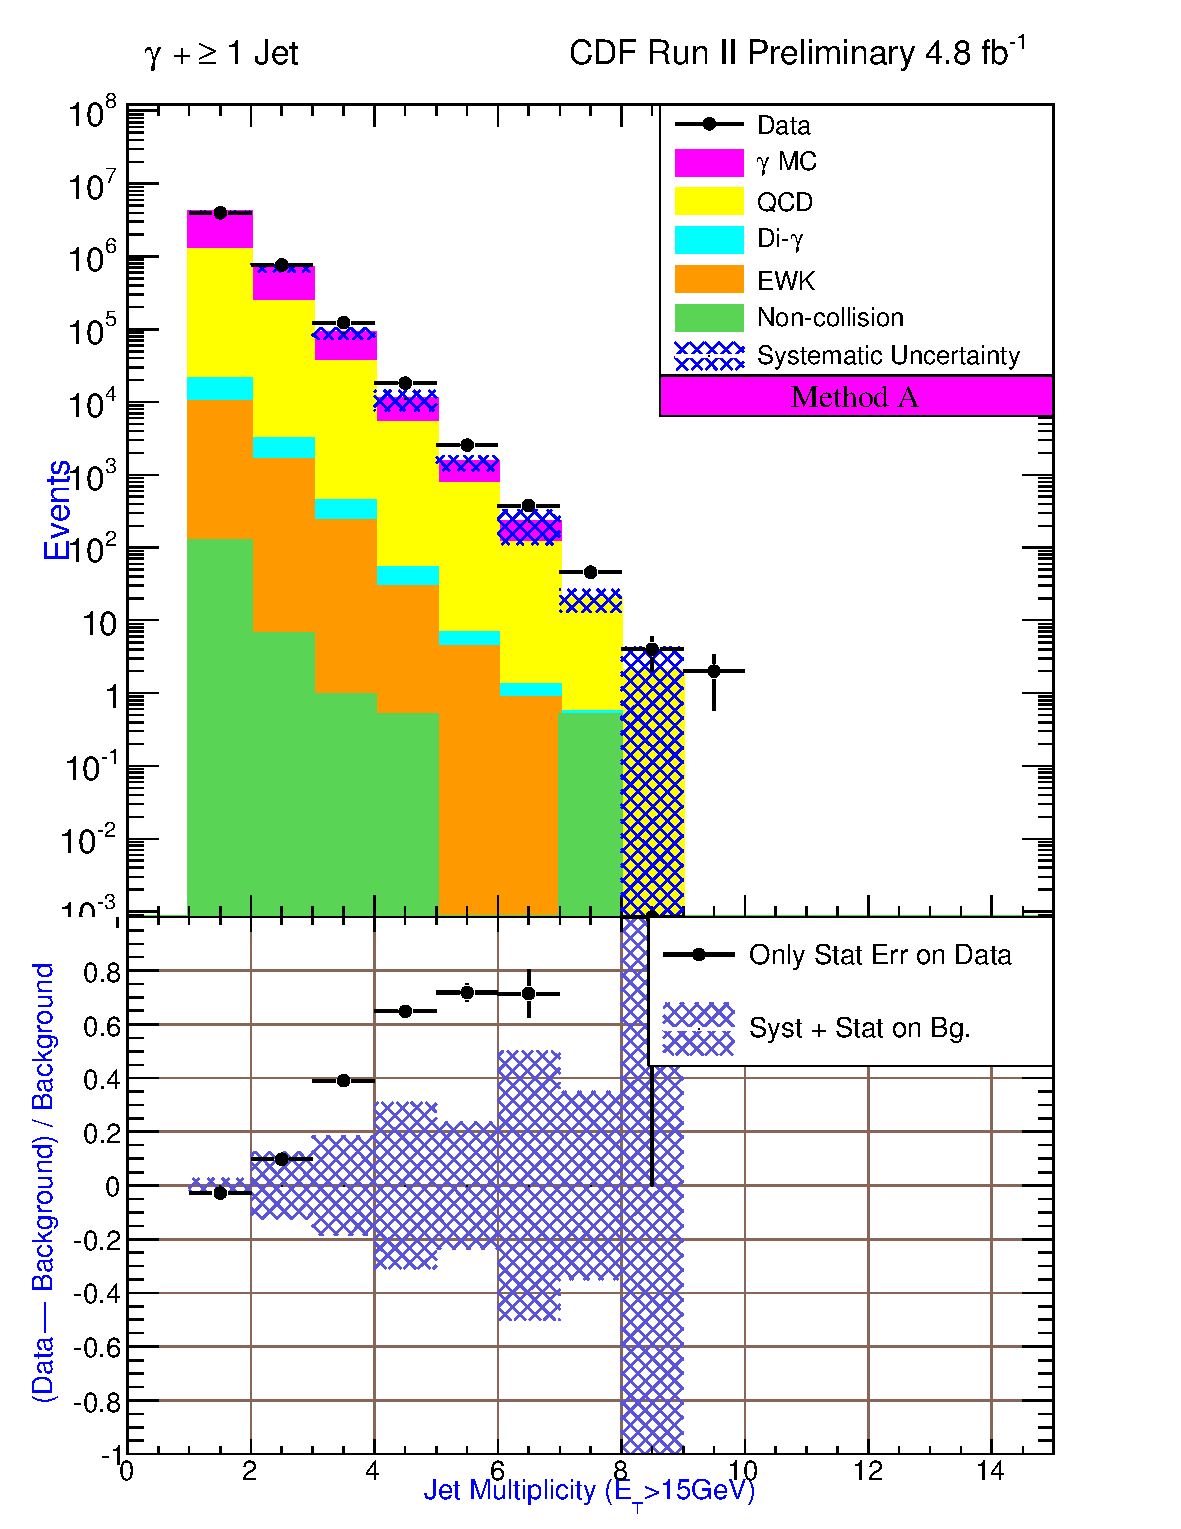
\includegraphics[keepaspectratio=true, scale=\resultsHistScale]{G30Jets_MtdA_plot1_NJet.pdf}\label{fig:pjSetTwo:NJet}}
\subfigure[]
{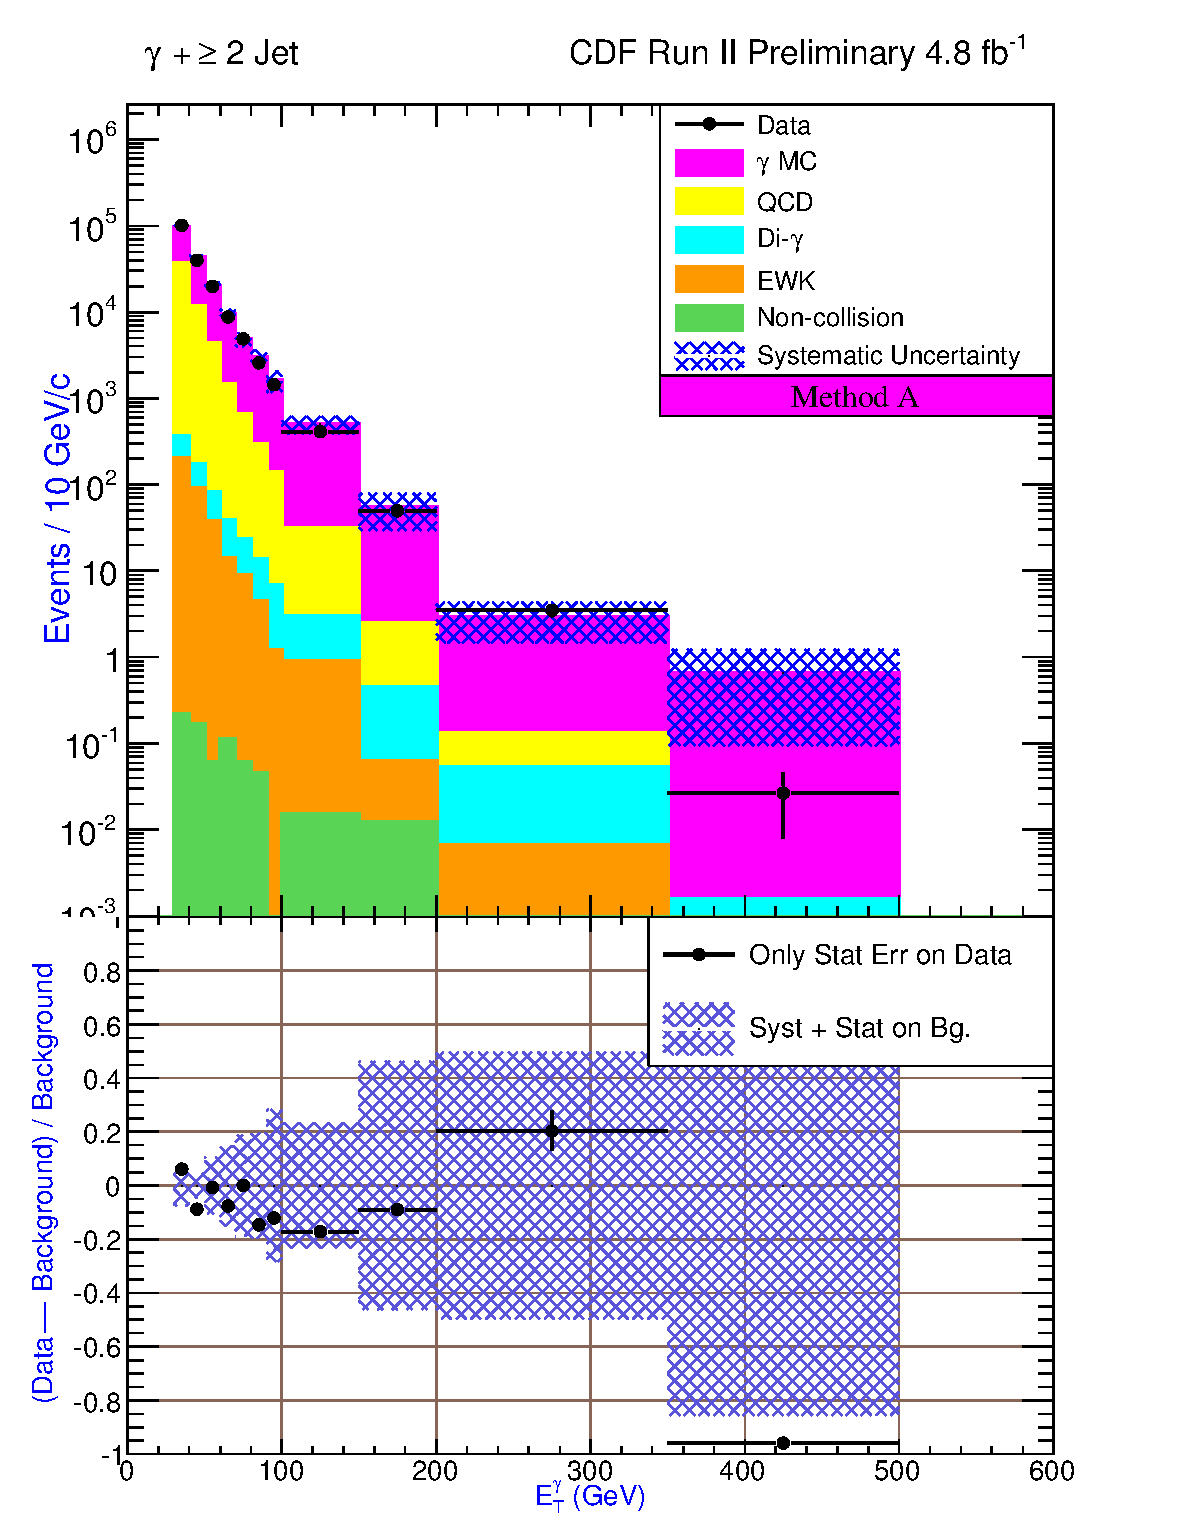
\includegraphics[keepaspectratio=true, scale=\resultsHistScale]{G30Jets_MtdA_plot2_Et_pho.pdf}}
\subfigure[]
{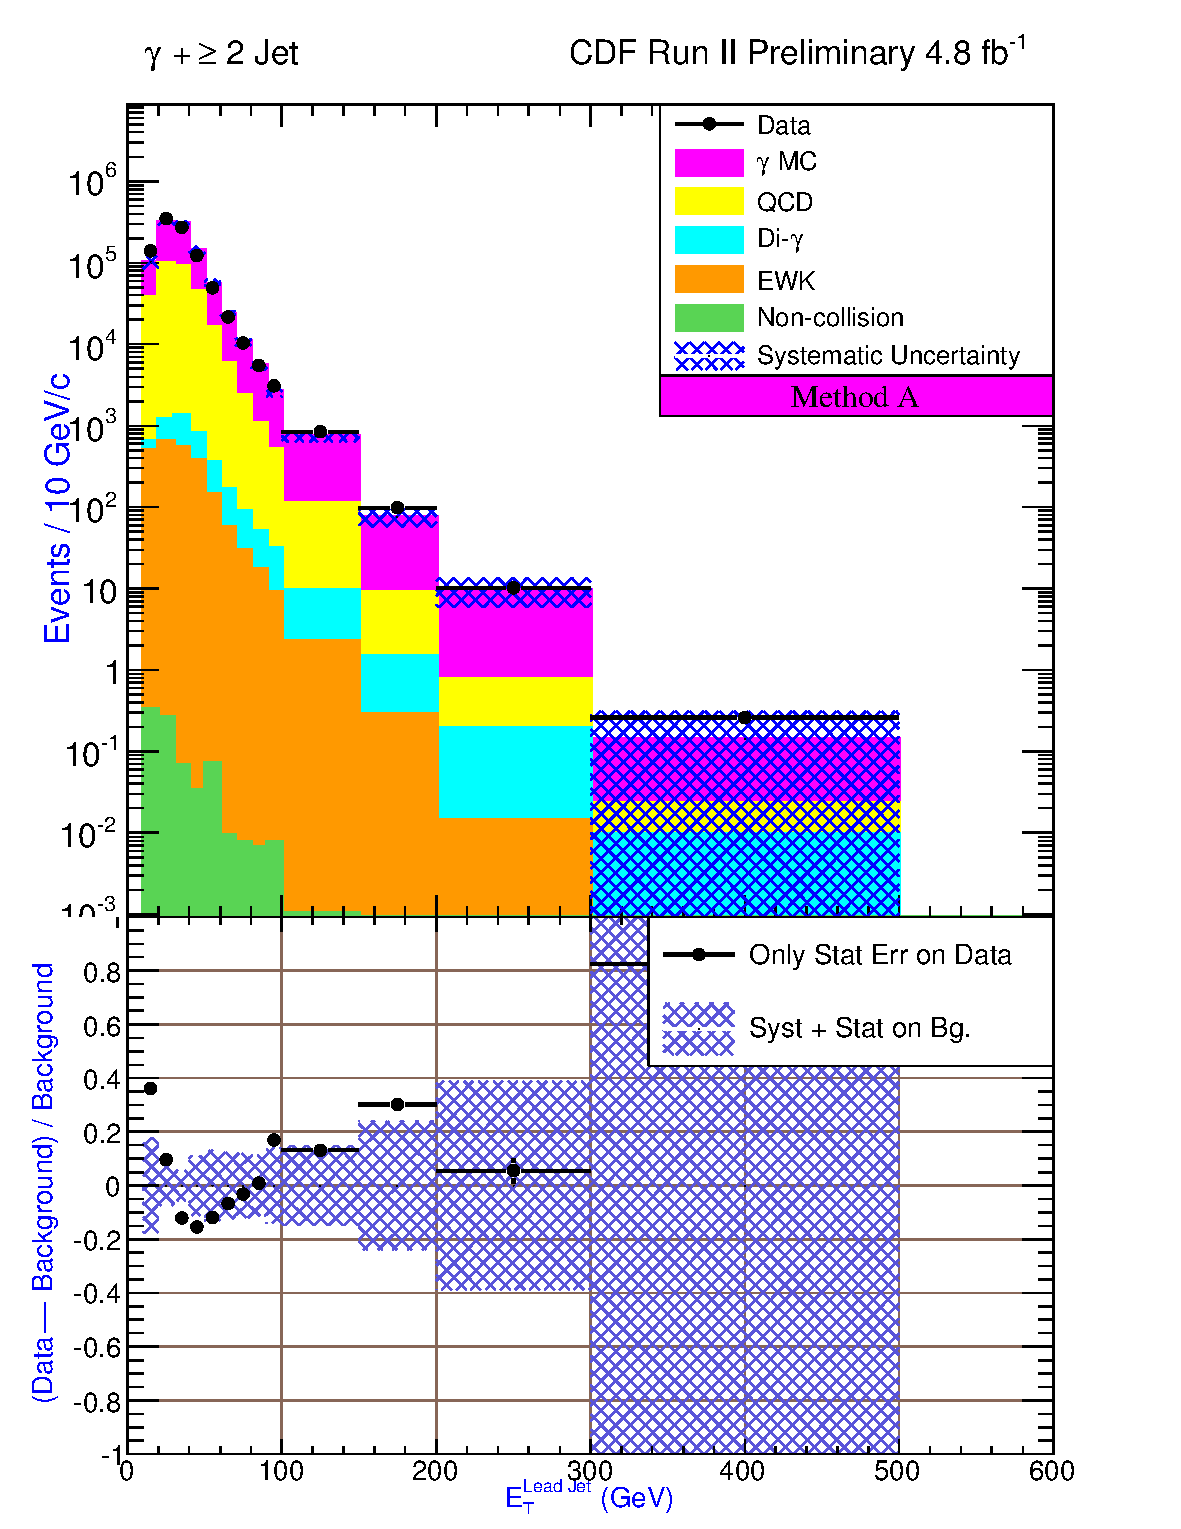
\includegraphics[keepaspectratio=true, scale=\resultsHistScale]{G30Jets_MtdA_plot2_Et_j1.pdf}}
\caption{Kinematic distributions of \phoonejet (top) and \photwojet (bottom) events using Method A. The beginning of Chapter~\ref{chp:Results} provides a description of the elements in these distributions.}
\label{fig:pjSetTwo}
\end{figure*}
\clearpage

\begin{figure*}[h!]
\centering
\subfigure[]
{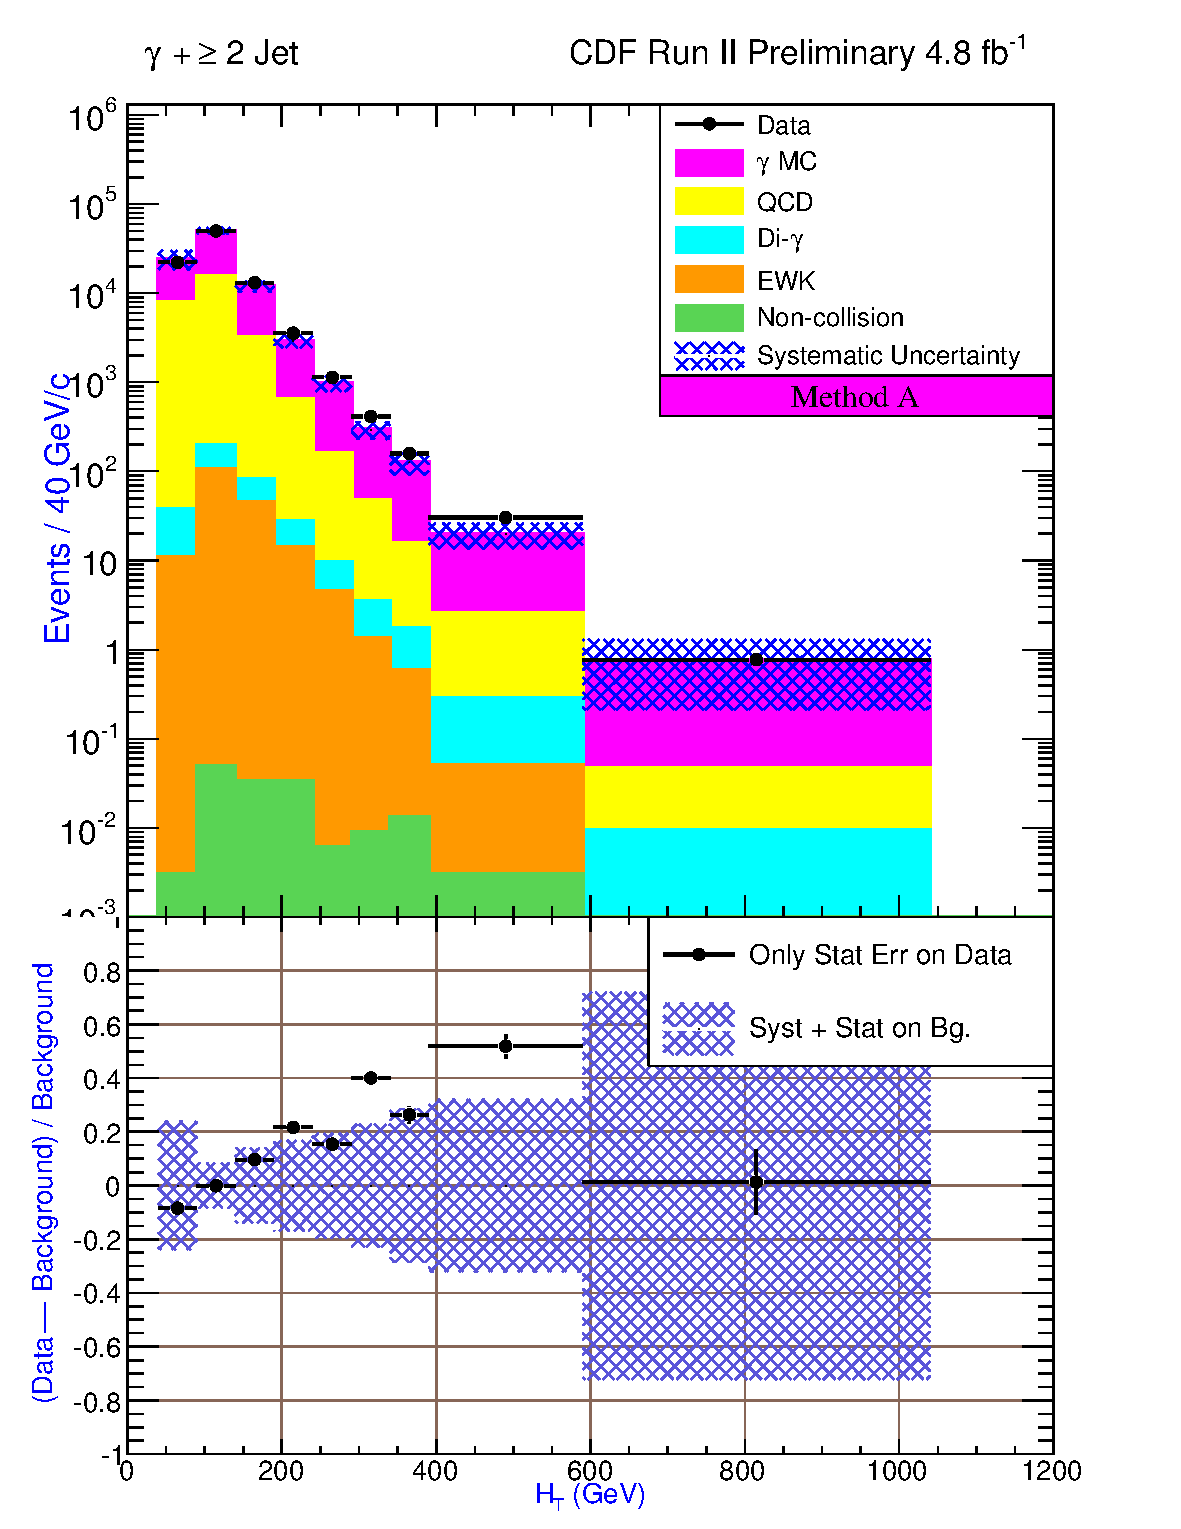
\includegraphics[keepaspectratio=true, scale=\resultsHistScale]{G30Jets_MtdA_plot2_Ht.pdf}}
\subfigure[]
{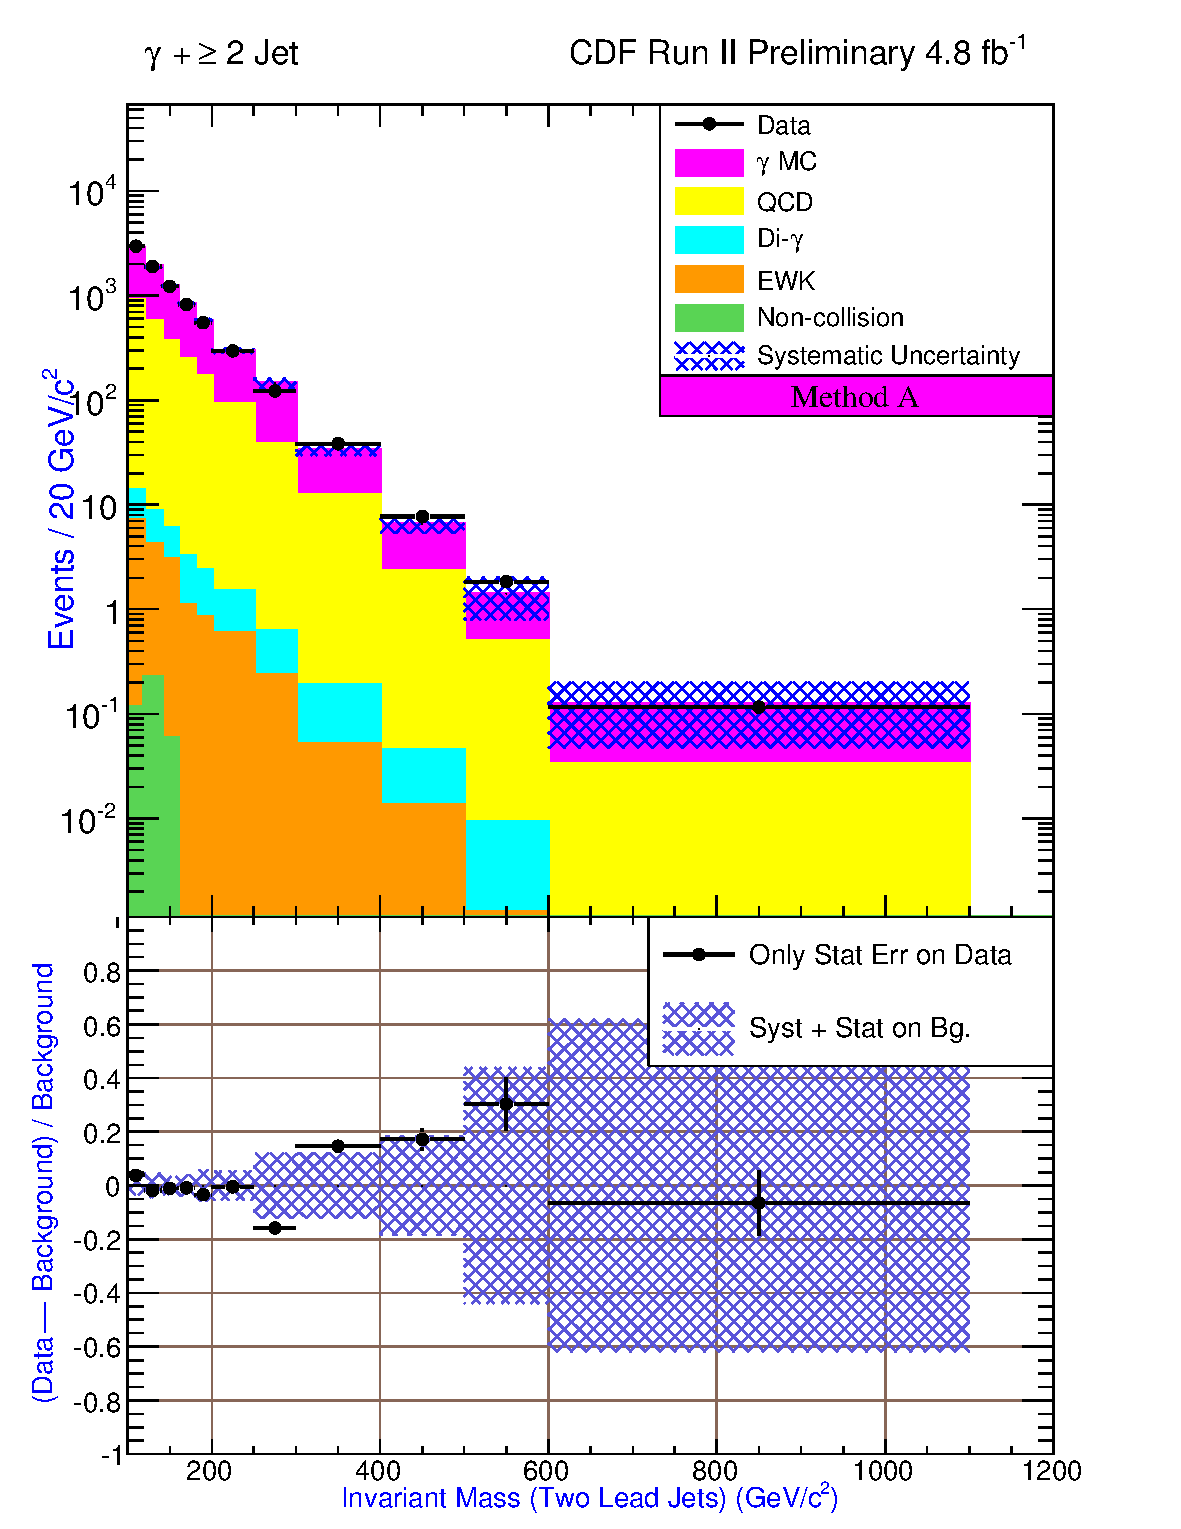
\includegraphics[keepaspectratio=true, scale=\resultsHistScale]{G30Jets_MtdA_plot2_InvMass_j1j2.pdf}}
\subfigure[]
{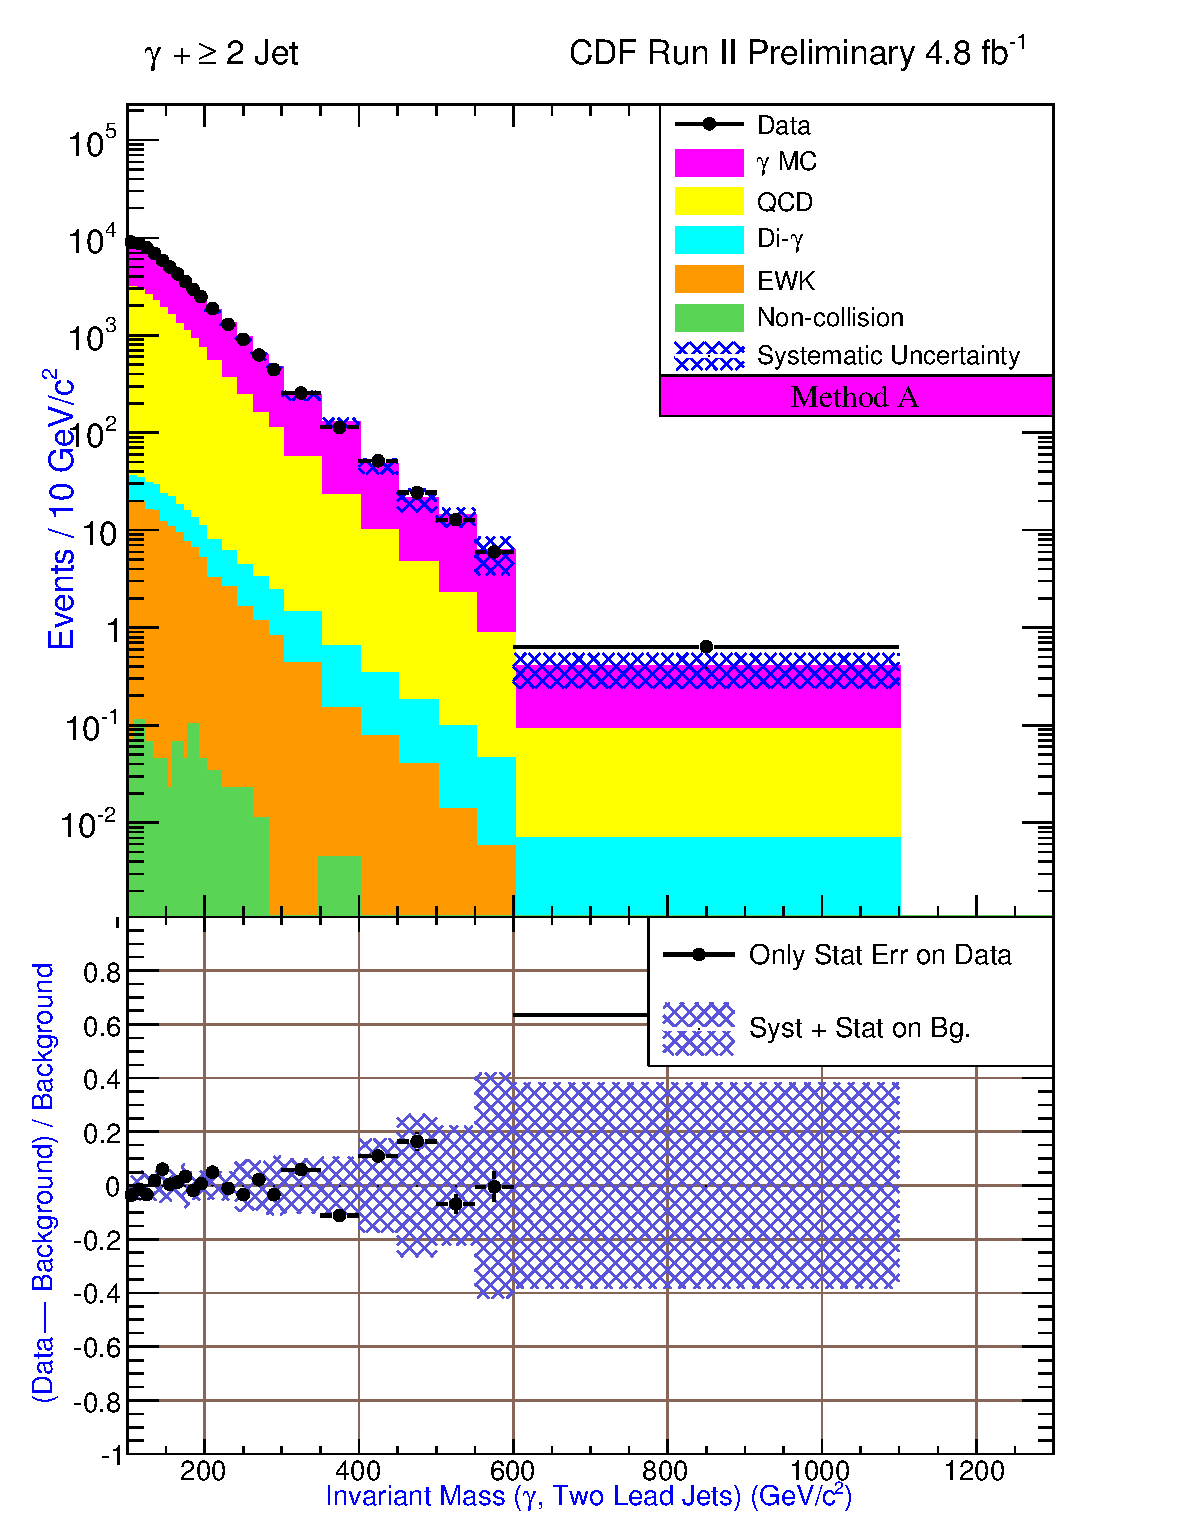
\includegraphics[keepaspectratio=true, scale=\resultsHistScale]{G30Jets_MtdA_plot2_InvMass_pj1j2.pdf}}
\subfigure[]
{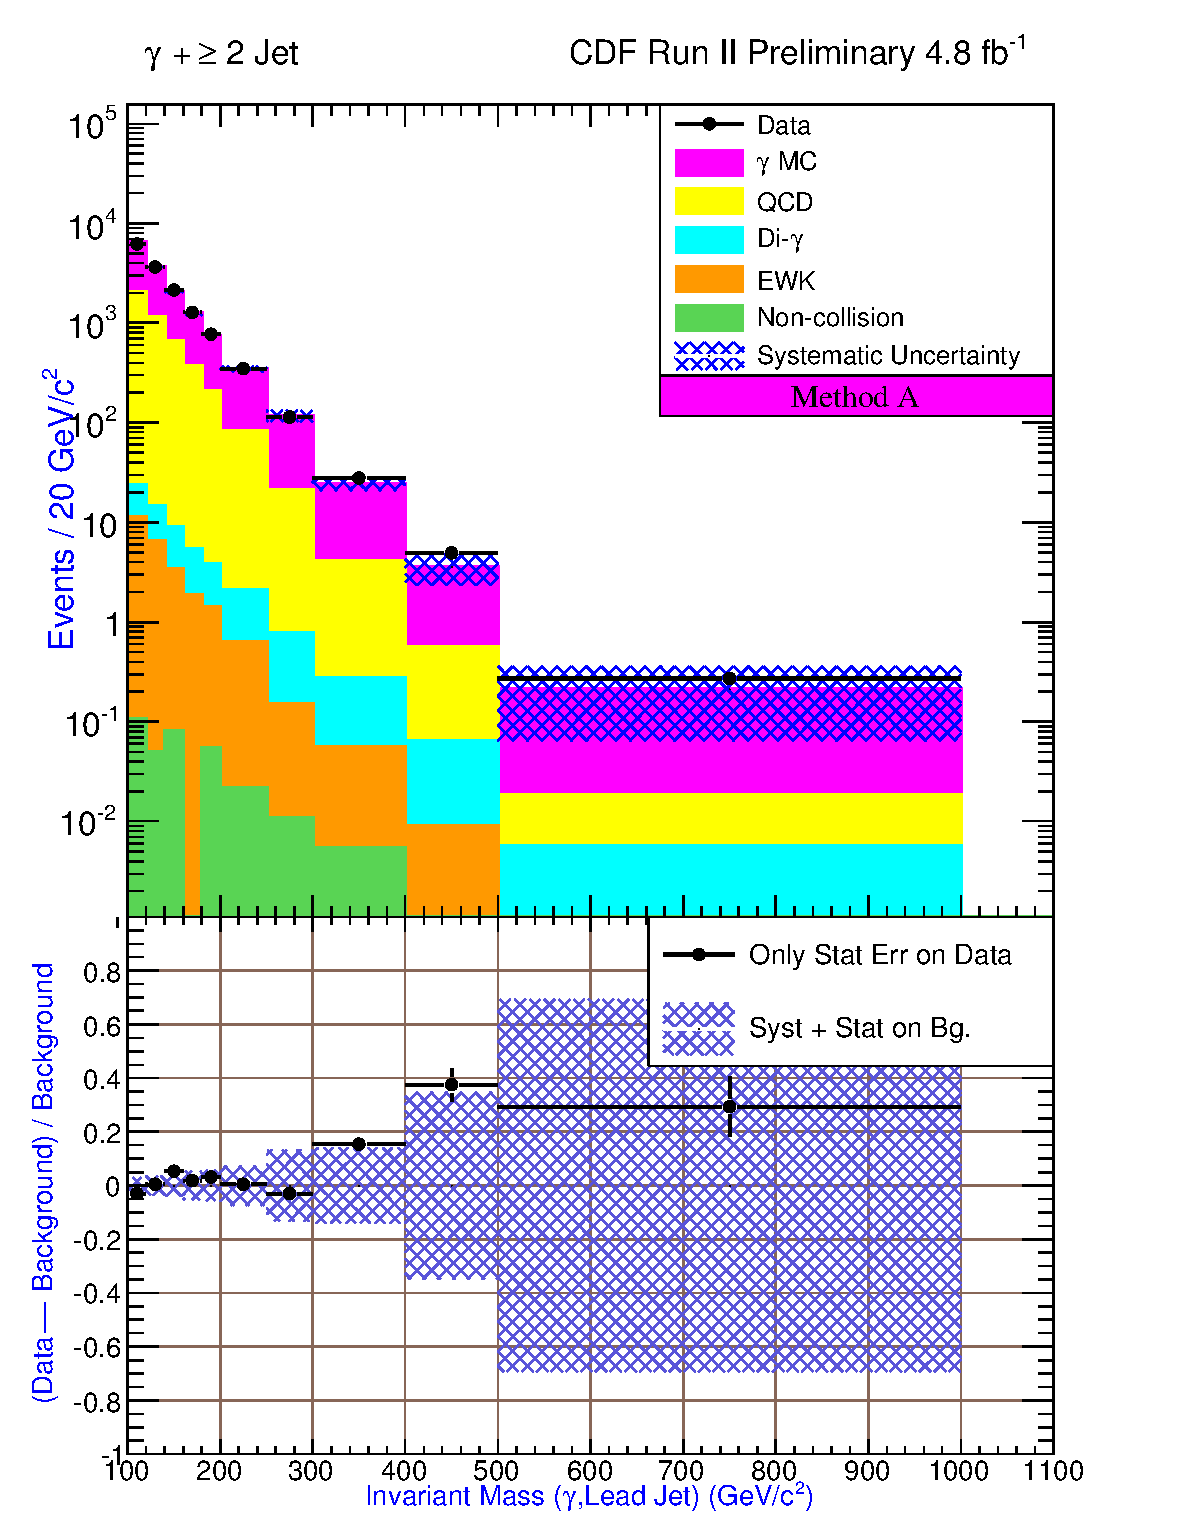
\includegraphics[keepaspectratio=true, scale=\resultsHistScale]{G30Jets_MtdA_plot2_InvMass_pj1.pdf}}
\caption{Kinematic distributions of \photwojet events using Method A. The beginning of Chapter~\ref{chp:Results} provides a description of the elements in these distributions.}
\label{fig:pjSetThree}
\end{figure*}
\clearpage

\begin{figure*}[h!]
\centering
\subfigure[]
{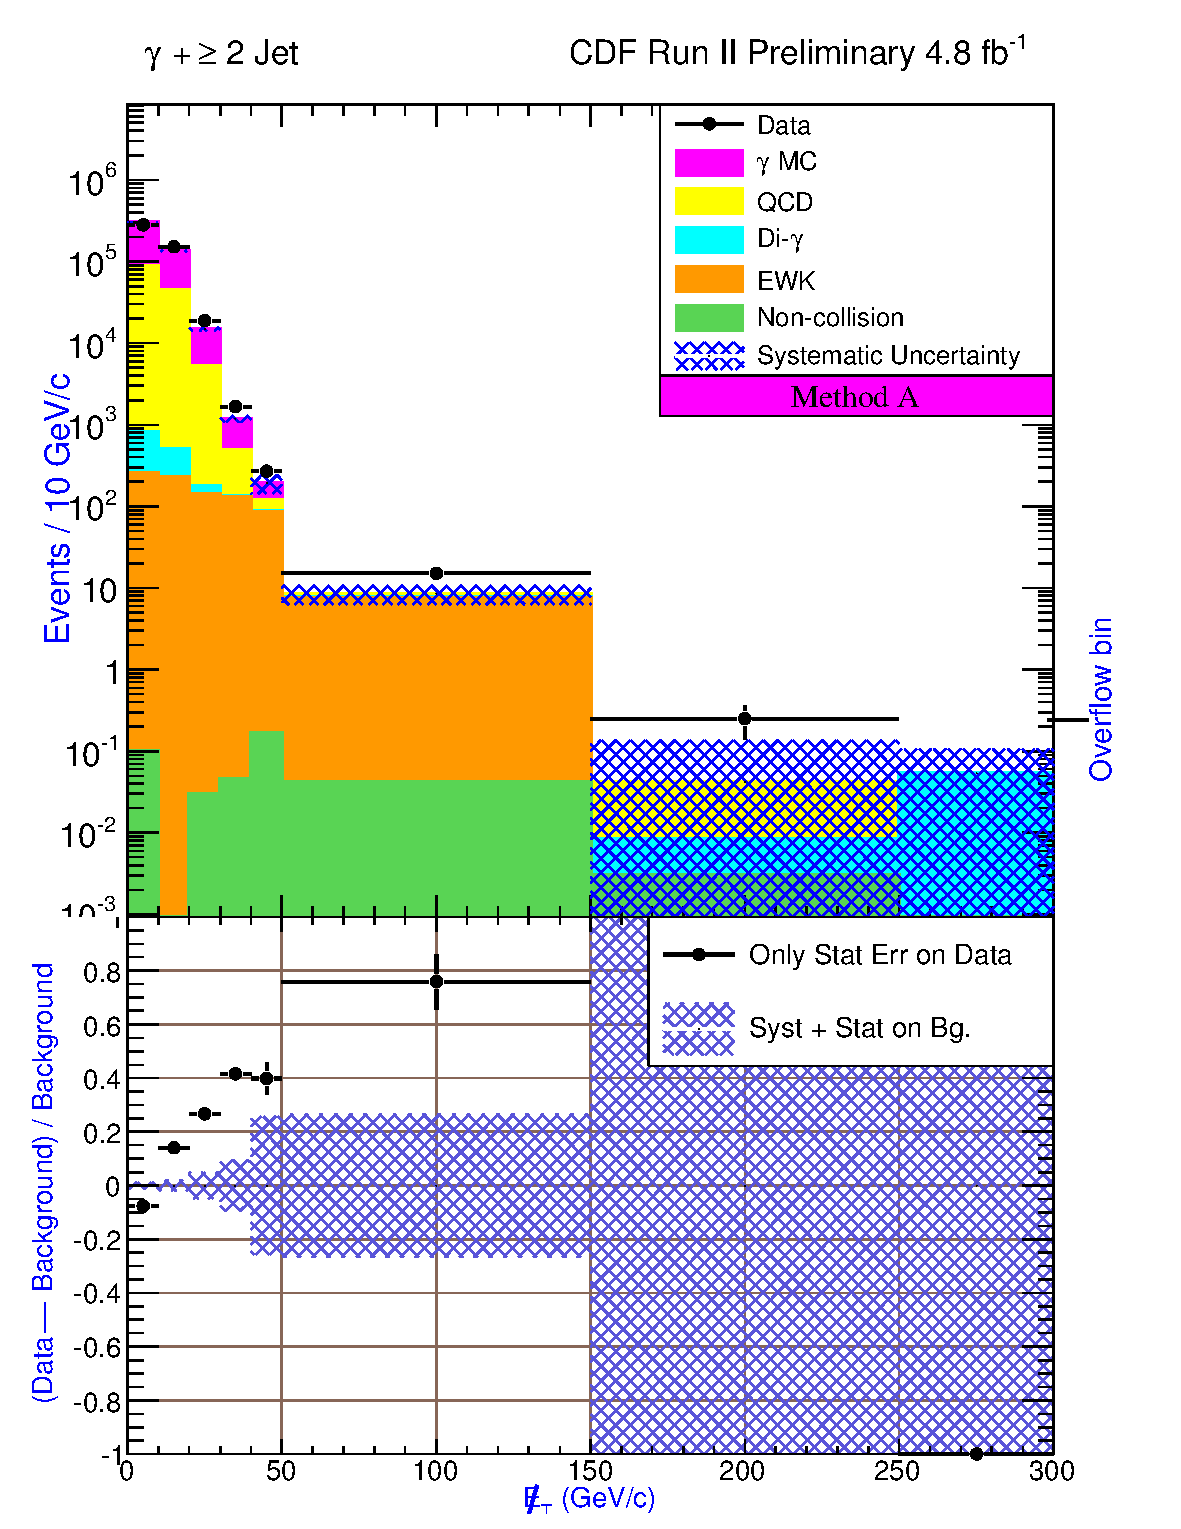
\includegraphics[keepaspectratio=true, scale=0.7]{G30Jets_MtdA_plot2_Met.pdf}}
\caption{Kinematic distributions of \photwojet events using Method A. The beginning of Chapter~\ref{chp:Results} provides a description of the elements in this distribution.}
\label{fig:pjSetFour}
\end{figure*}
\clearpage

%%%%%%%%%%%%%%%%%%%%%%%%%%%%%% METHOD A: G30 JETS+MET>20
\begin{figure*}[h!]
\centering
\subfigure[]
{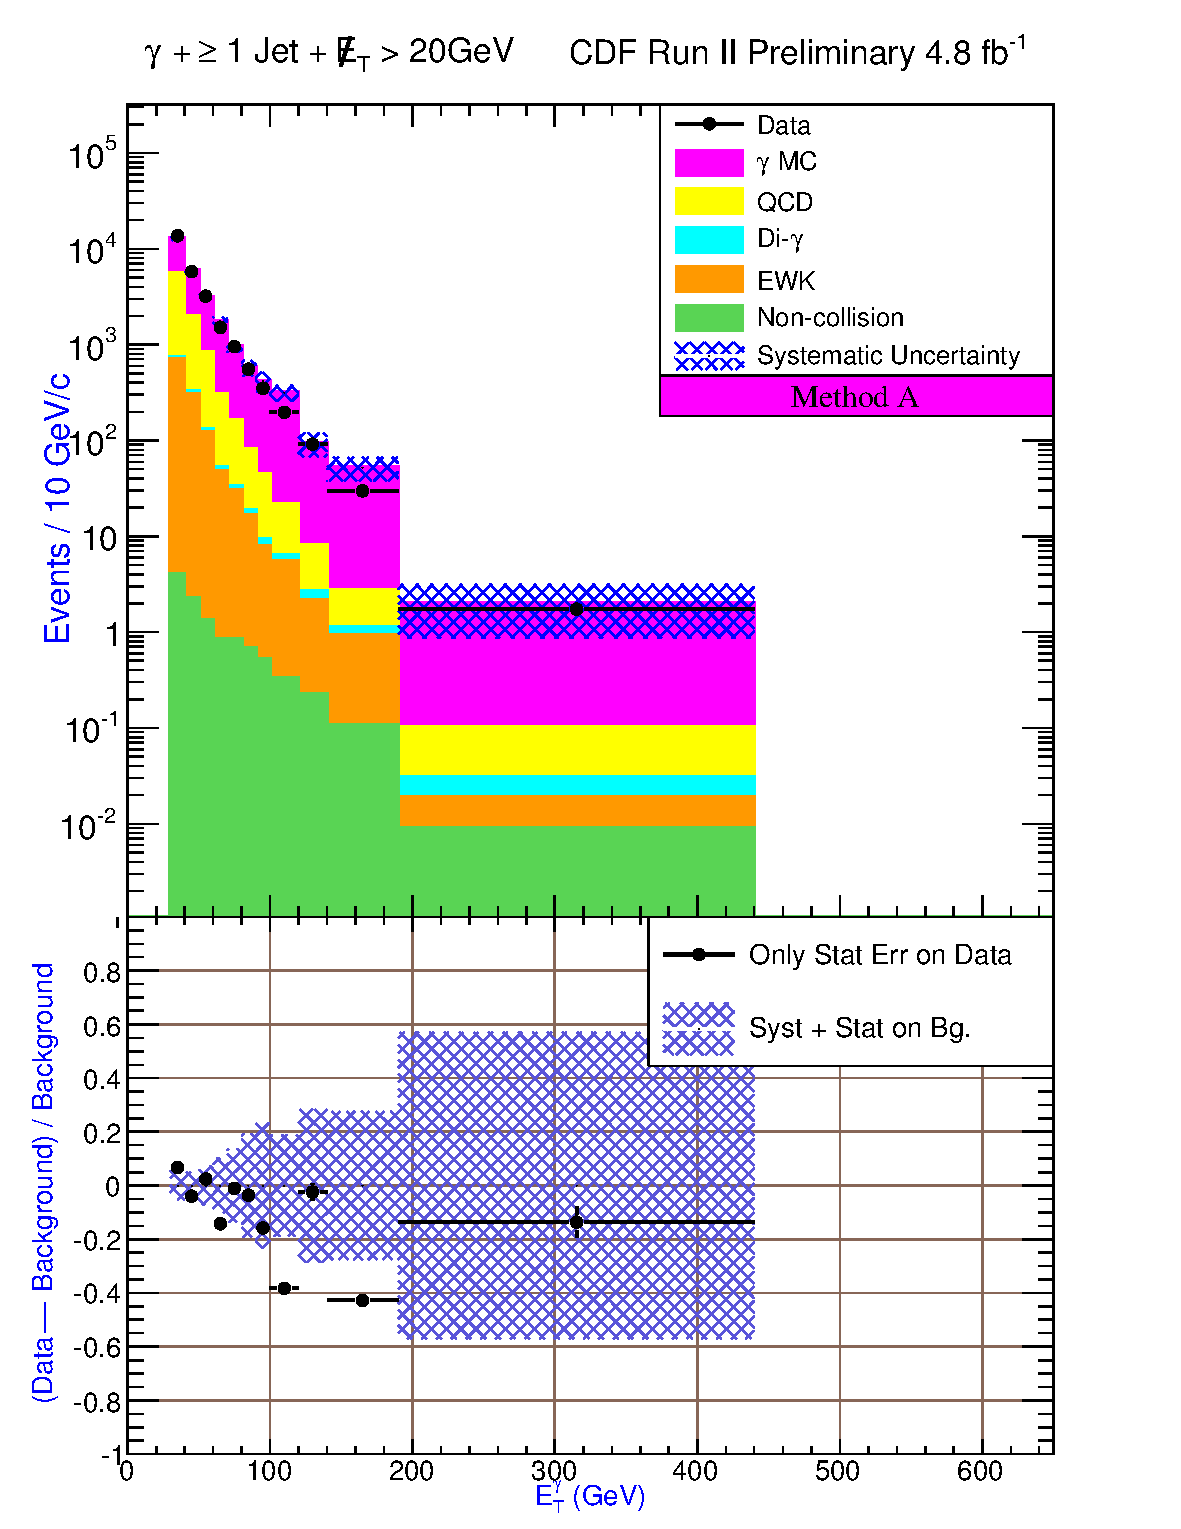
\includegraphics[keepaspectratio=true, scale=\resultsHistScale]{G30JetsMet20_MtdA_plot1_Et_pho.pdf}}
\subfigure[]
{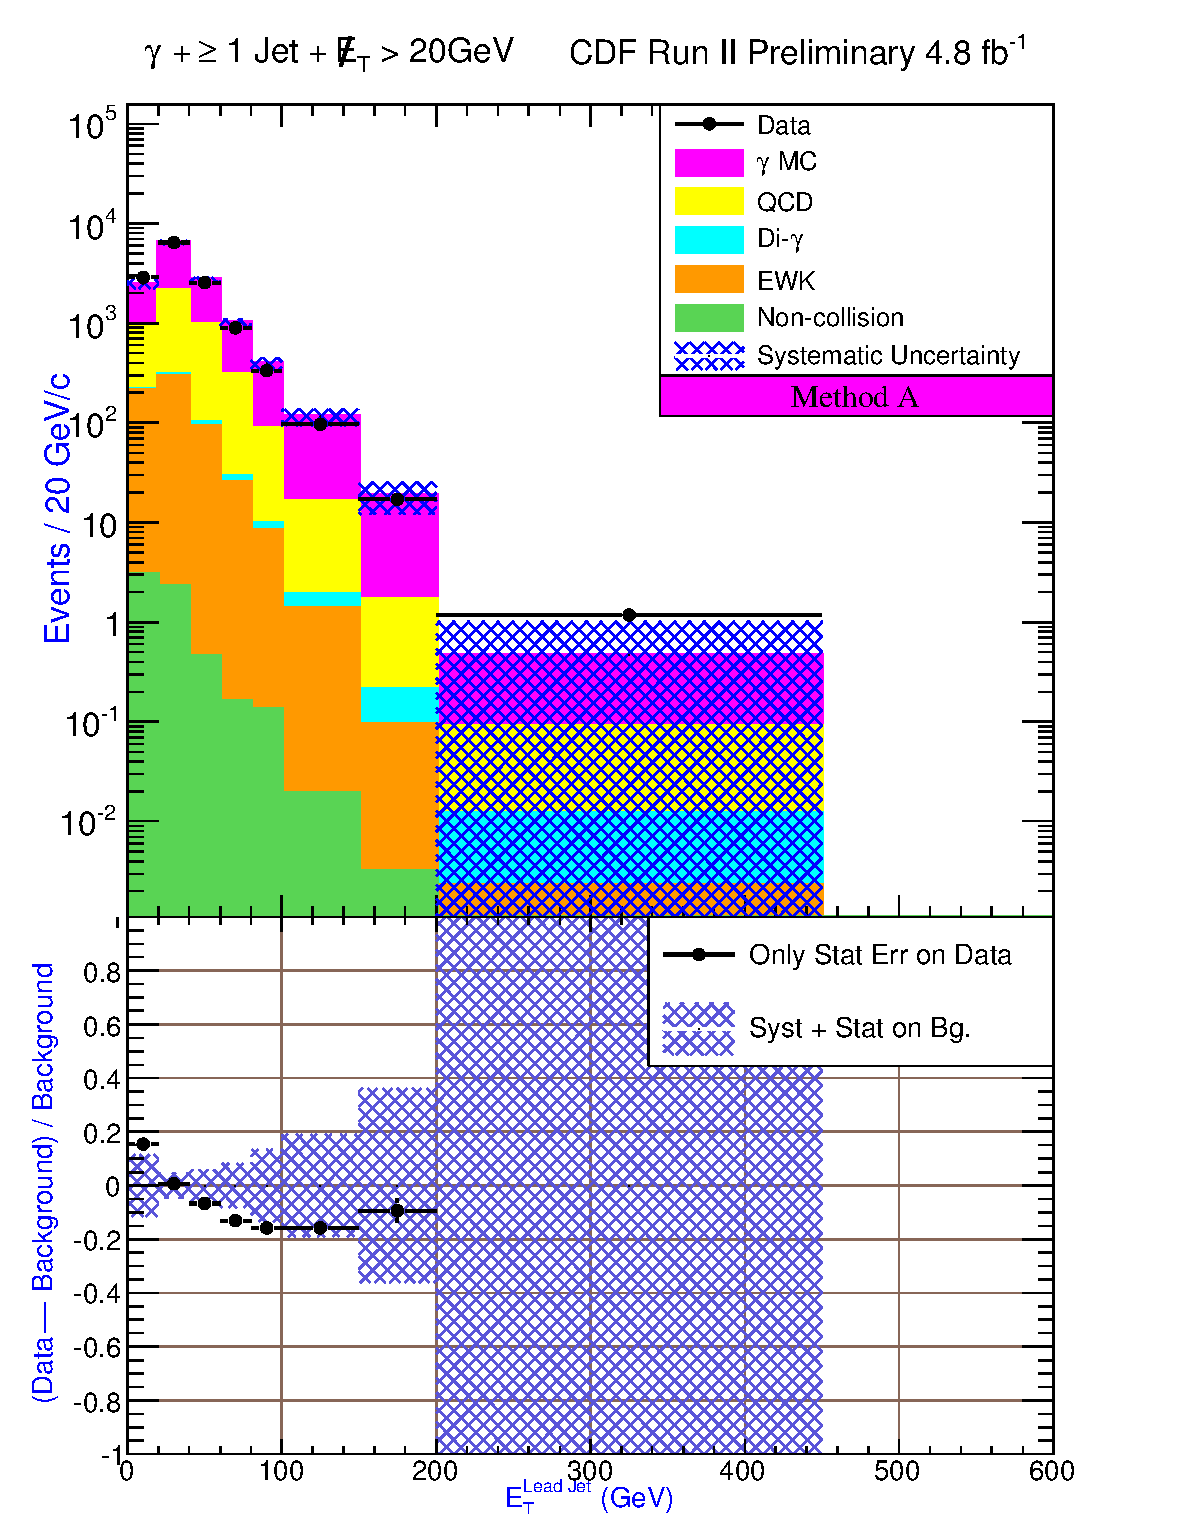
\includegraphics[keepaspectratio=true, scale=\resultsHistScale]{G30JetsMet20_MtdA_plot1_Et_j1.pdf}
}

\subfigure[]
{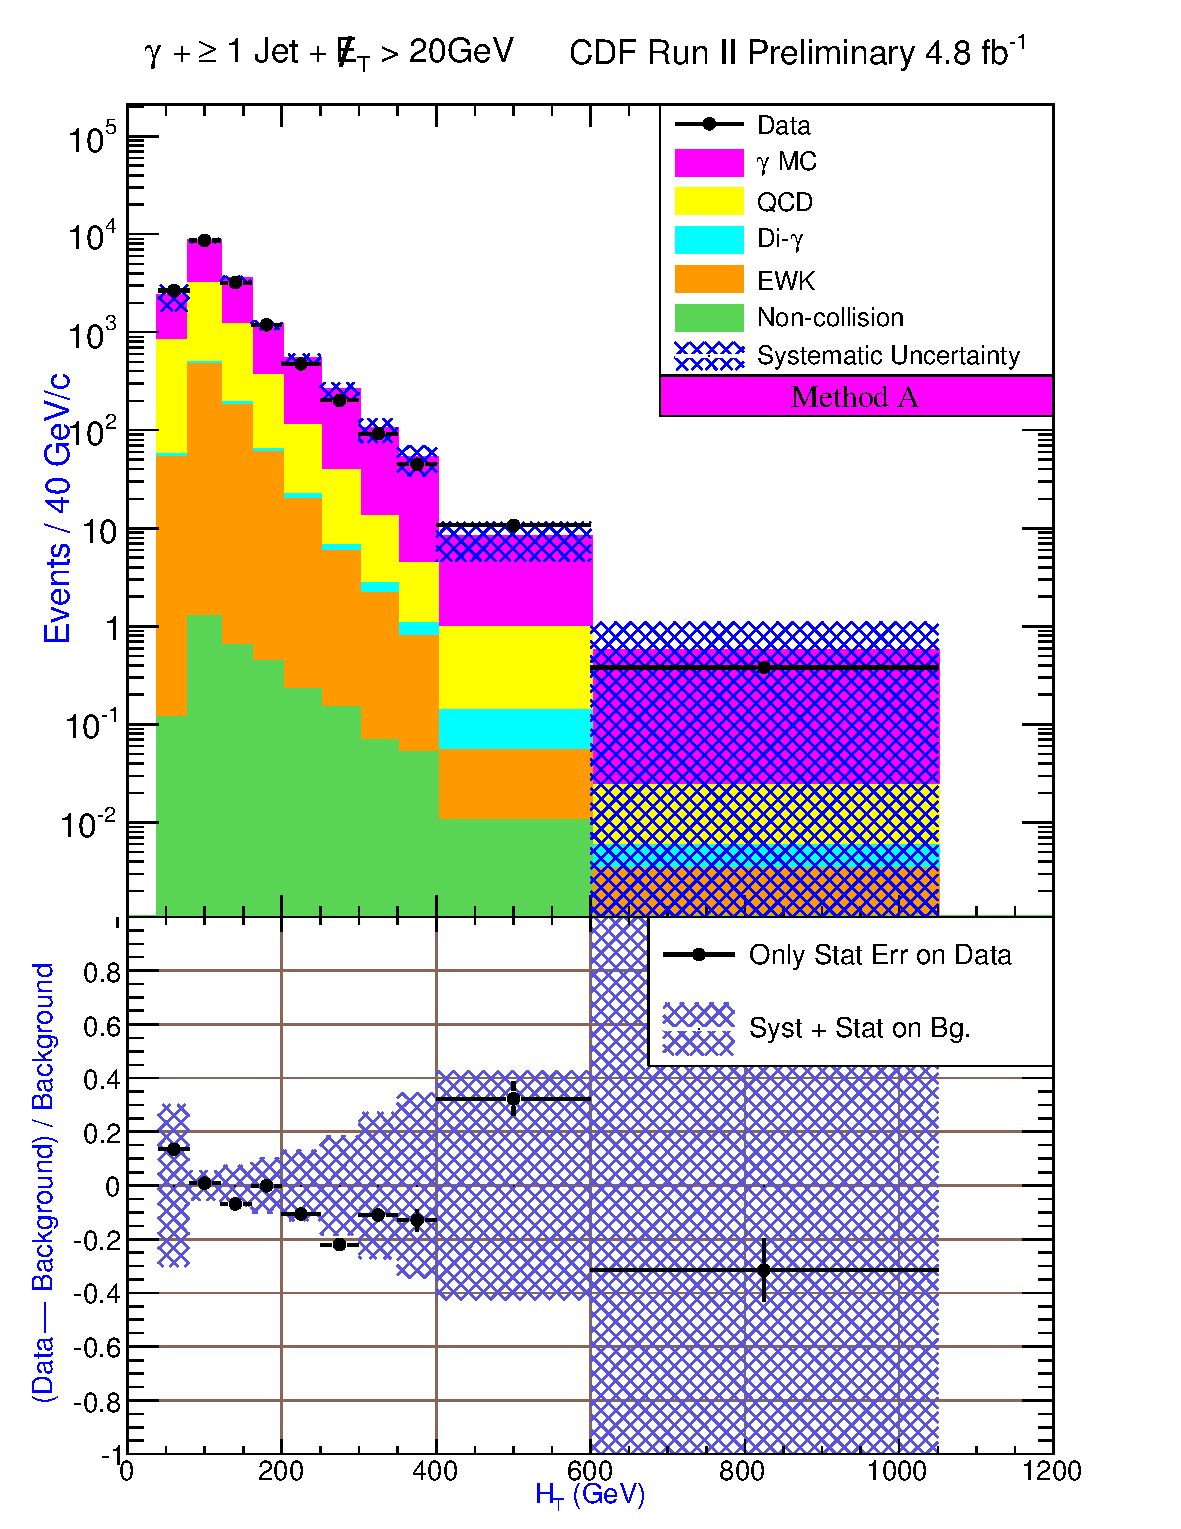
\includegraphics[keepaspectratio=true, scale=\resultsHistScale]{G30JetsMet20_MtdA_plot1_Ht.pdf}}
\subfigure[]
{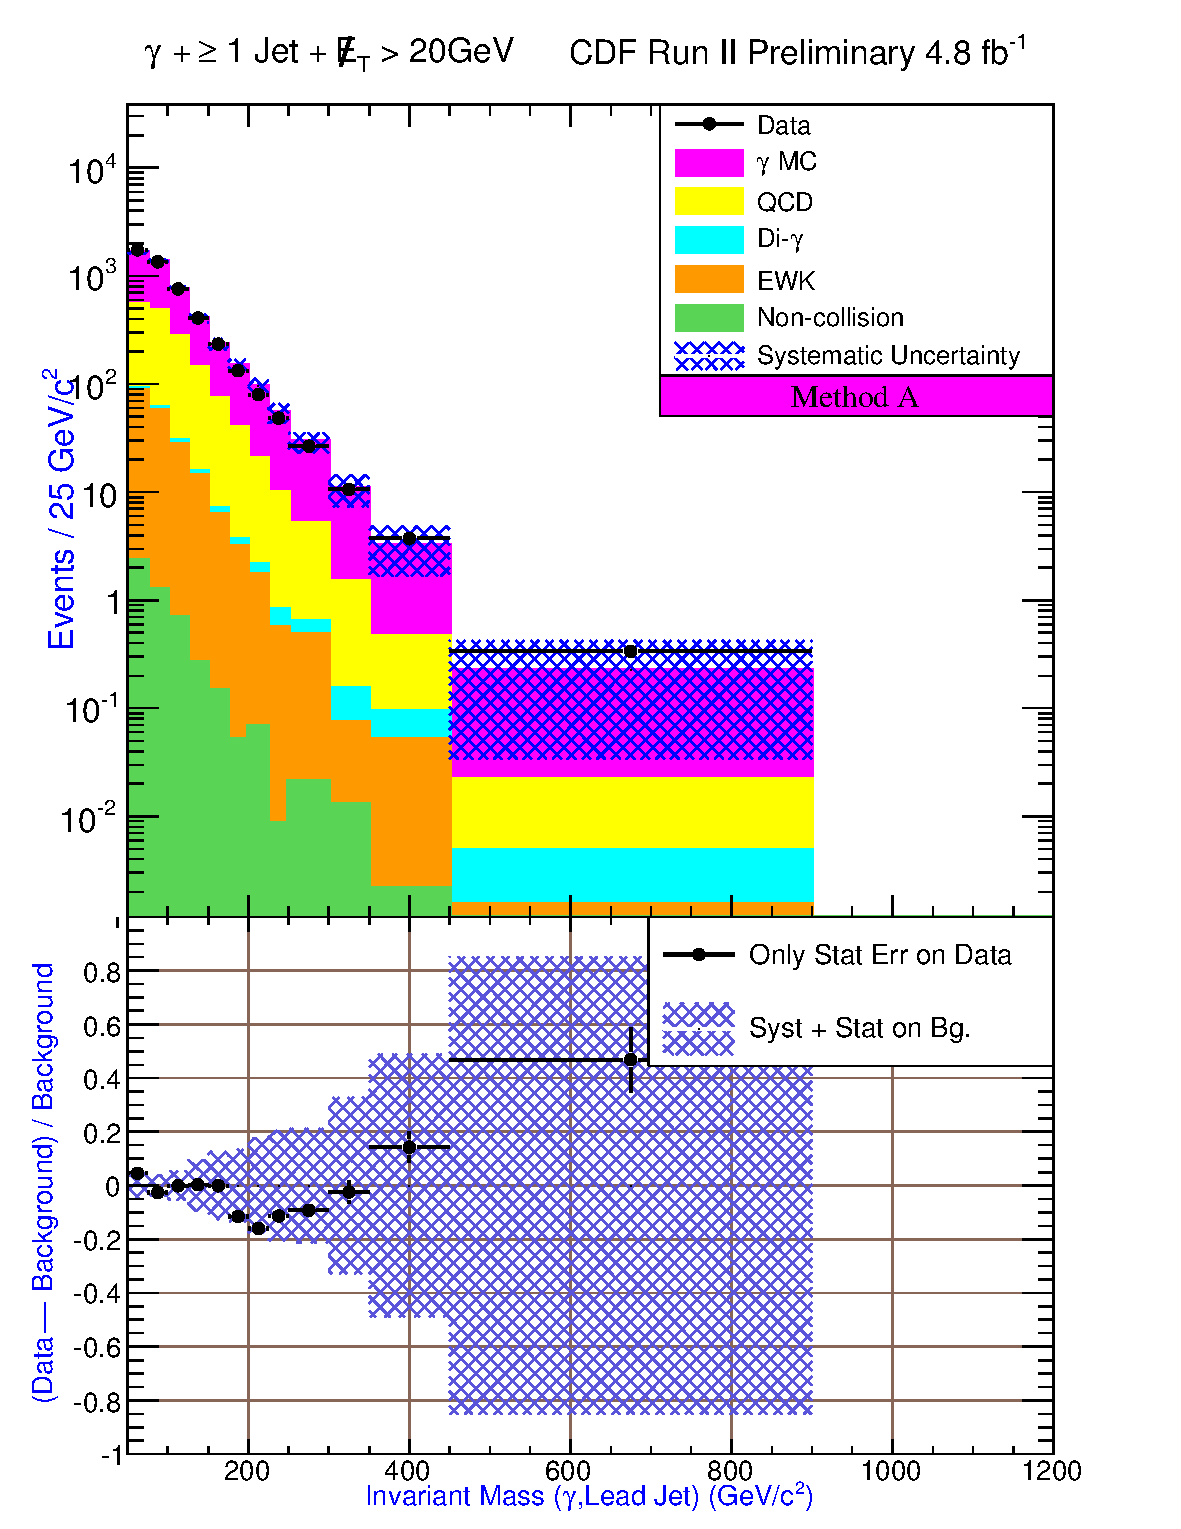
\includegraphics[keepaspectratio=true, scale=\resultsHistScale]{G30JetsMet20_MtdA_plot1_InvMass_pj1.pdf}}
\caption{Kinematic distributions of \phoonejet + \met$>$~20~\etUnits events using \mbox{Method A}. The beginning of Chapter~\ref{chp:Results} provides a description of the elements in these distributions.}
\label{fig:pjMetSetOne}
\end{figure*}
\clearpage

\begin{figure*}[h!]
\centering
\subfigure[]
{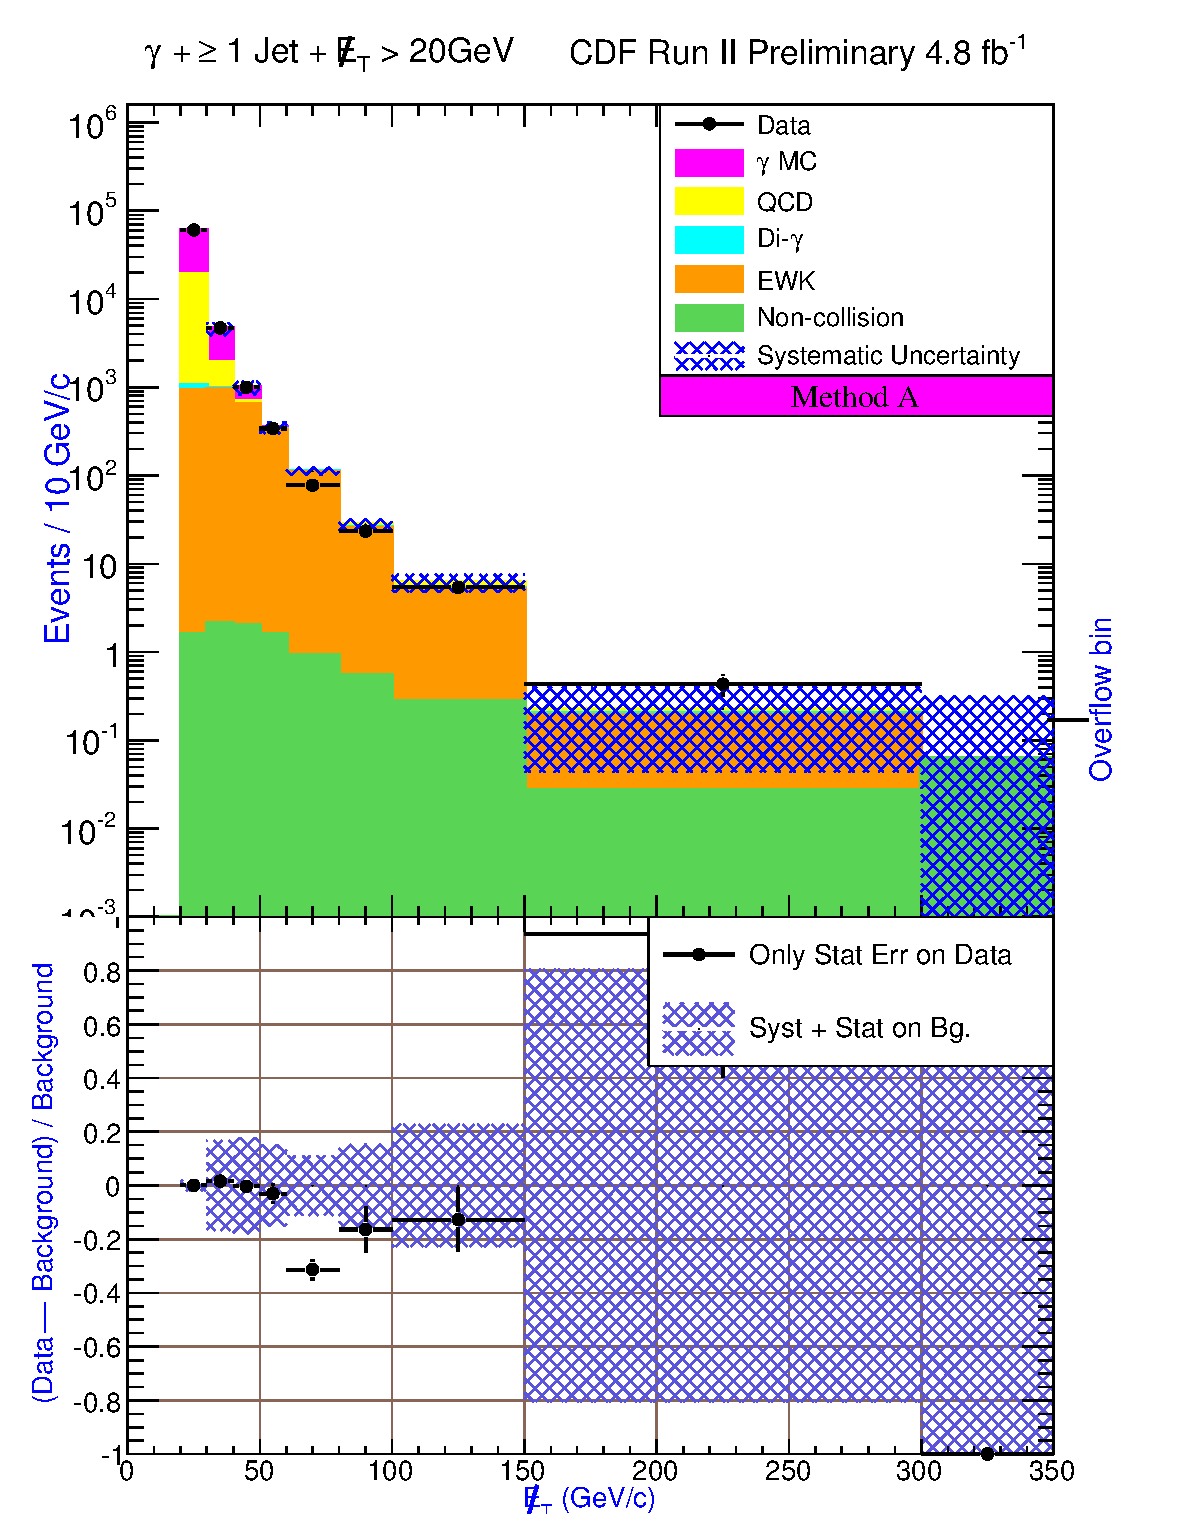
\includegraphics[keepaspectratio=true, scale=\resultsHistScale]{G30JetsMet20_MtdA_plot1_Met.pdf}}
\subfigure[]
{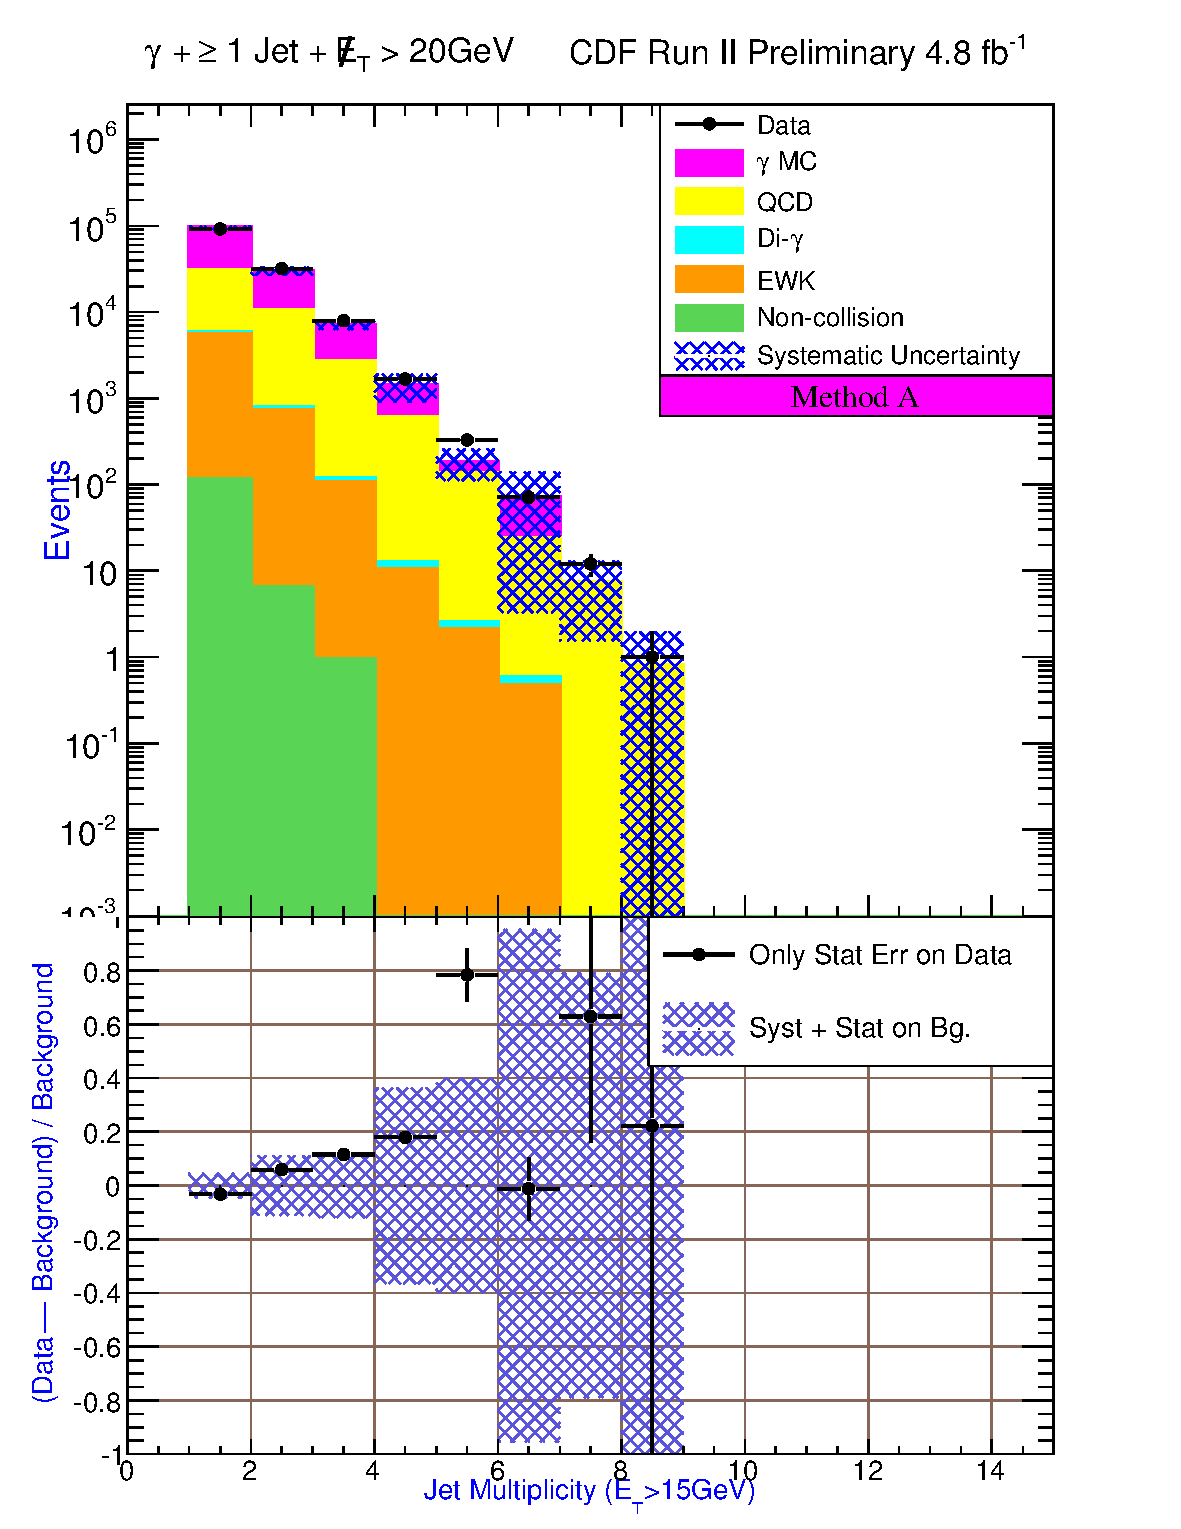
\includegraphics[keepaspectratio=true, scale=\resultsHistScale]{G30JetsMet20_MtdA_plot1_NJet.pdf}}
\subfigure[]
{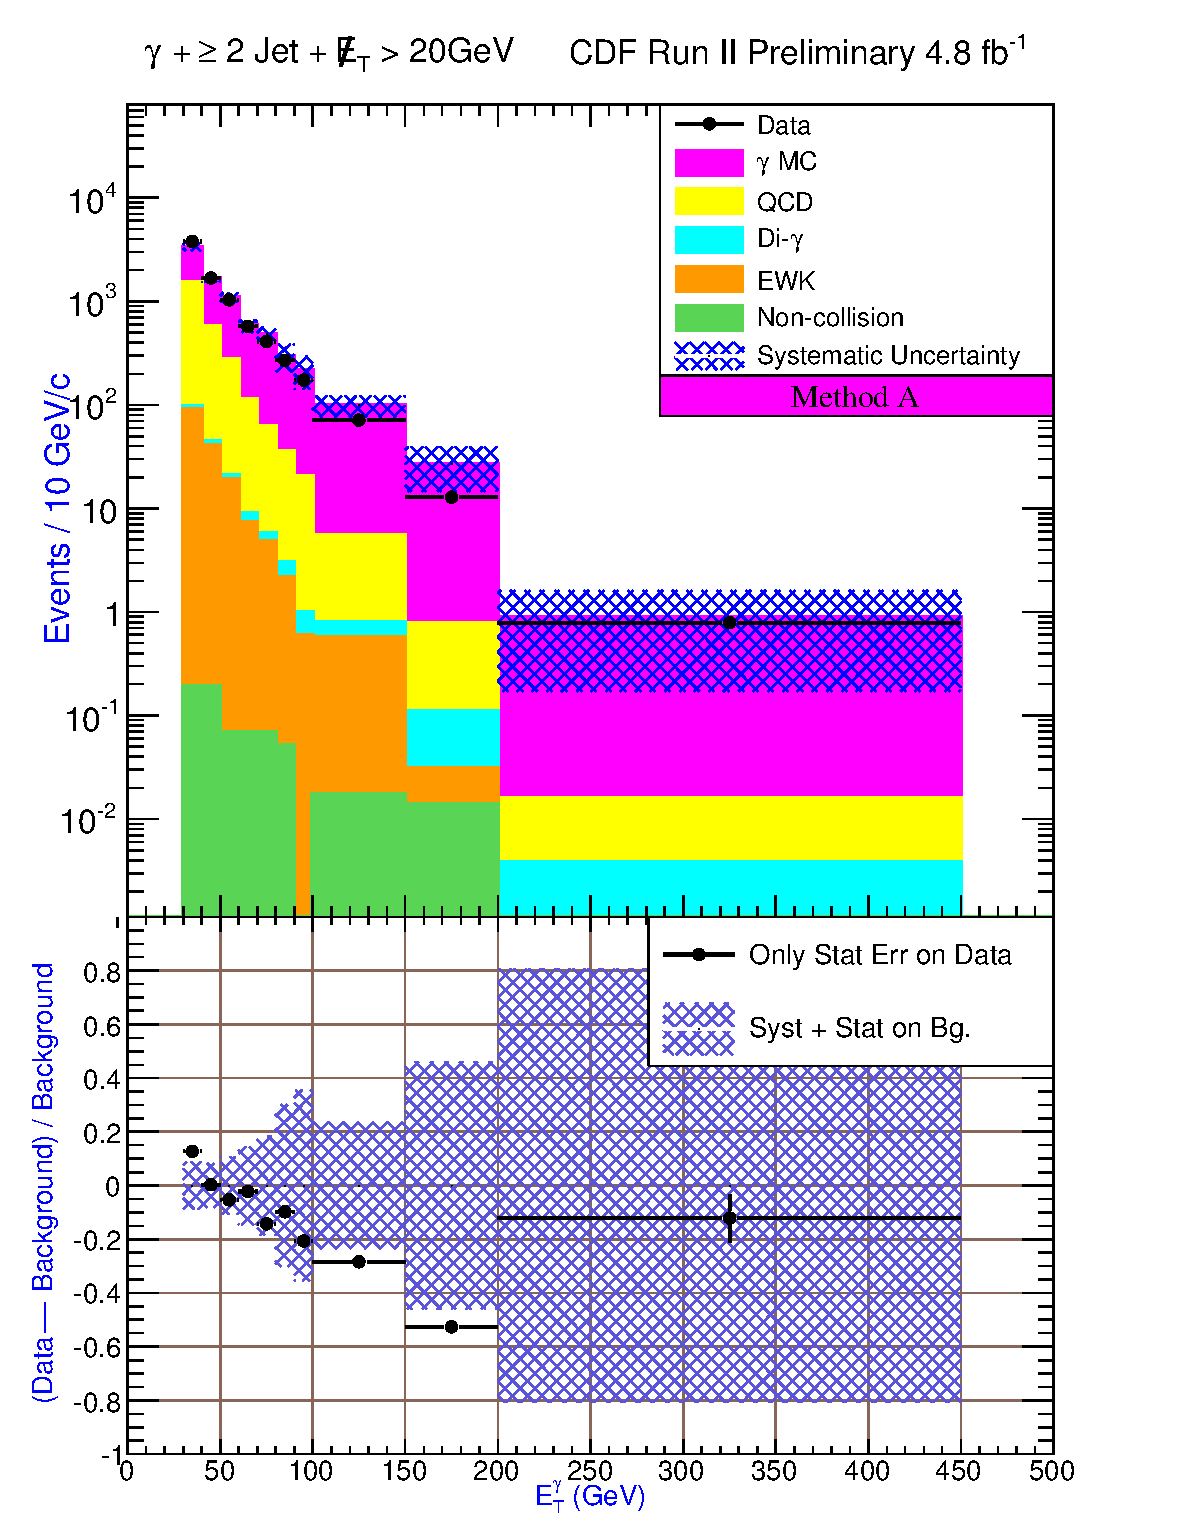
\includegraphics[keepaspectratio=true, scale=\resultsHistScale]{G30JetsMet20_MtdA_plot2_Et_pho.pdf}}
\subfigure[]
{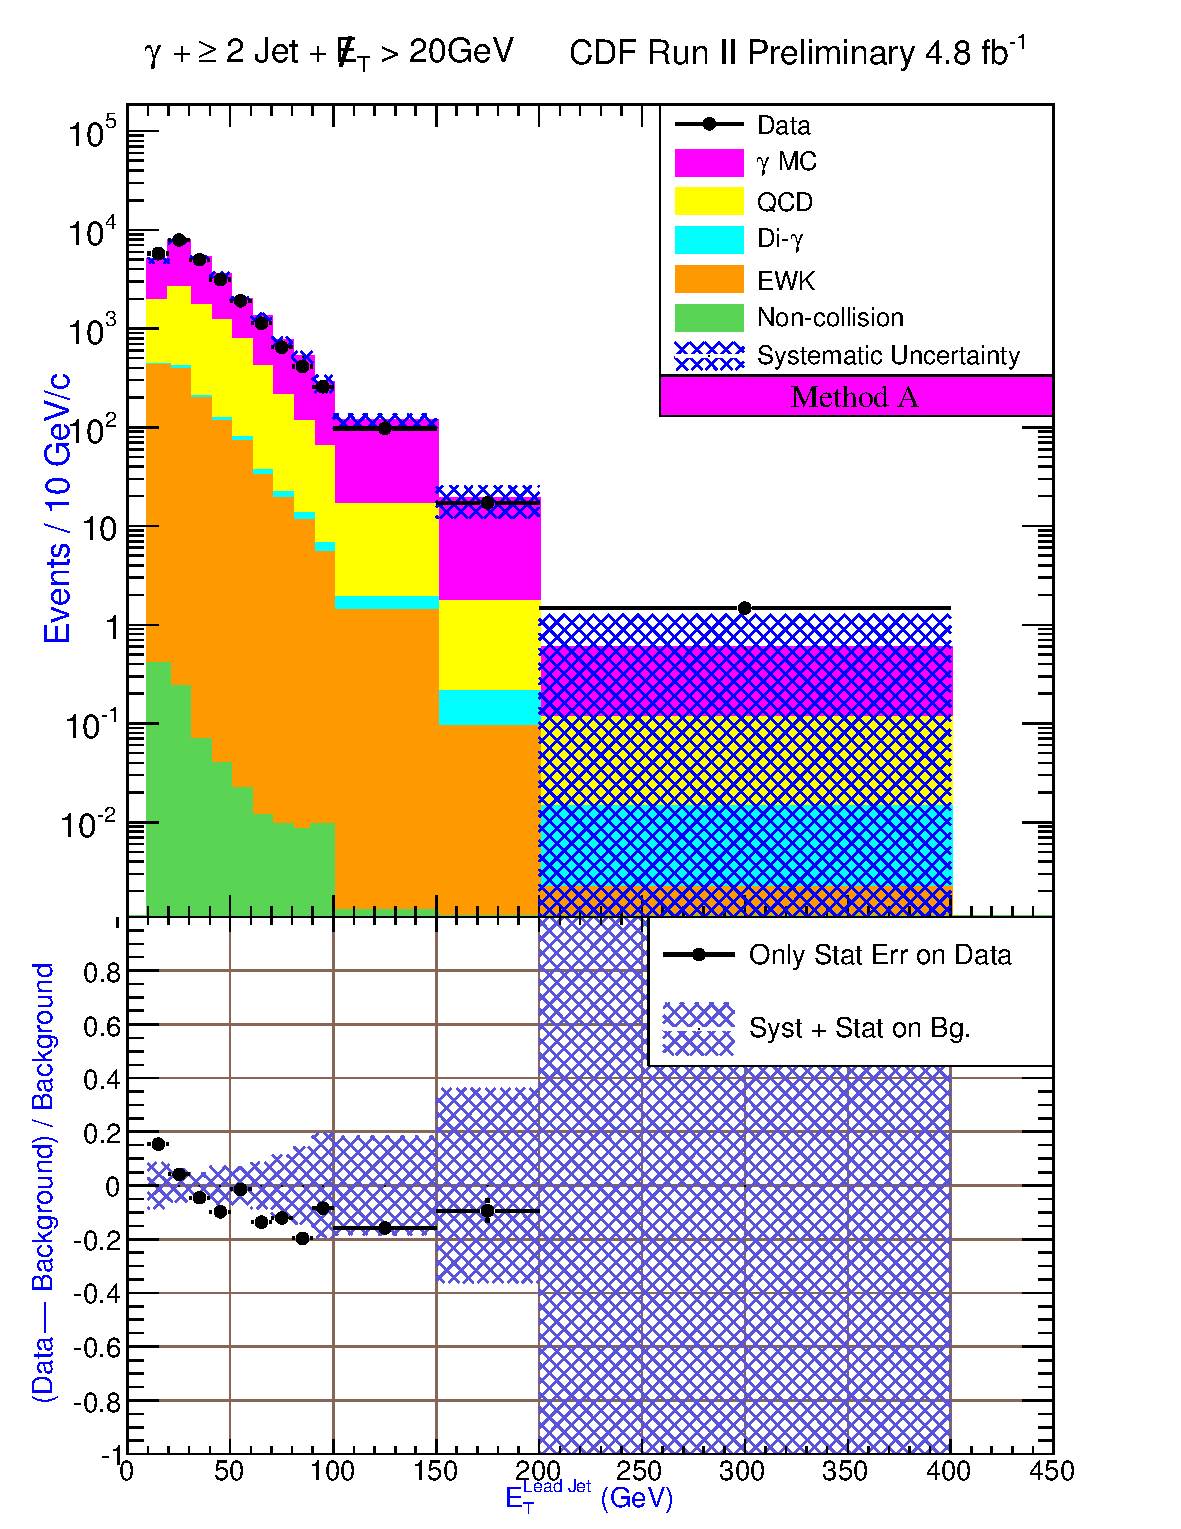
\includegraphics[keepaspectratio=true, scale=\resultsHistScale]{G30JetsMet20_MtdA_plot2_Et_j1.pdf}}
\caption{Kinematic distributions of \phoonejet + \met$>$~20~\etUnits (top) and \photwojet + \met$>$~20~\etUnits (bottom) events using Method A. The beginning of Chapter~\ref{chp:Results} provides a description of the elements in these distributions.}
\label{fig:pjMetSetTwo}
\end{figure*}
\clearpage

\begin{figure*}[h!]
\centering
\subfigure[]
{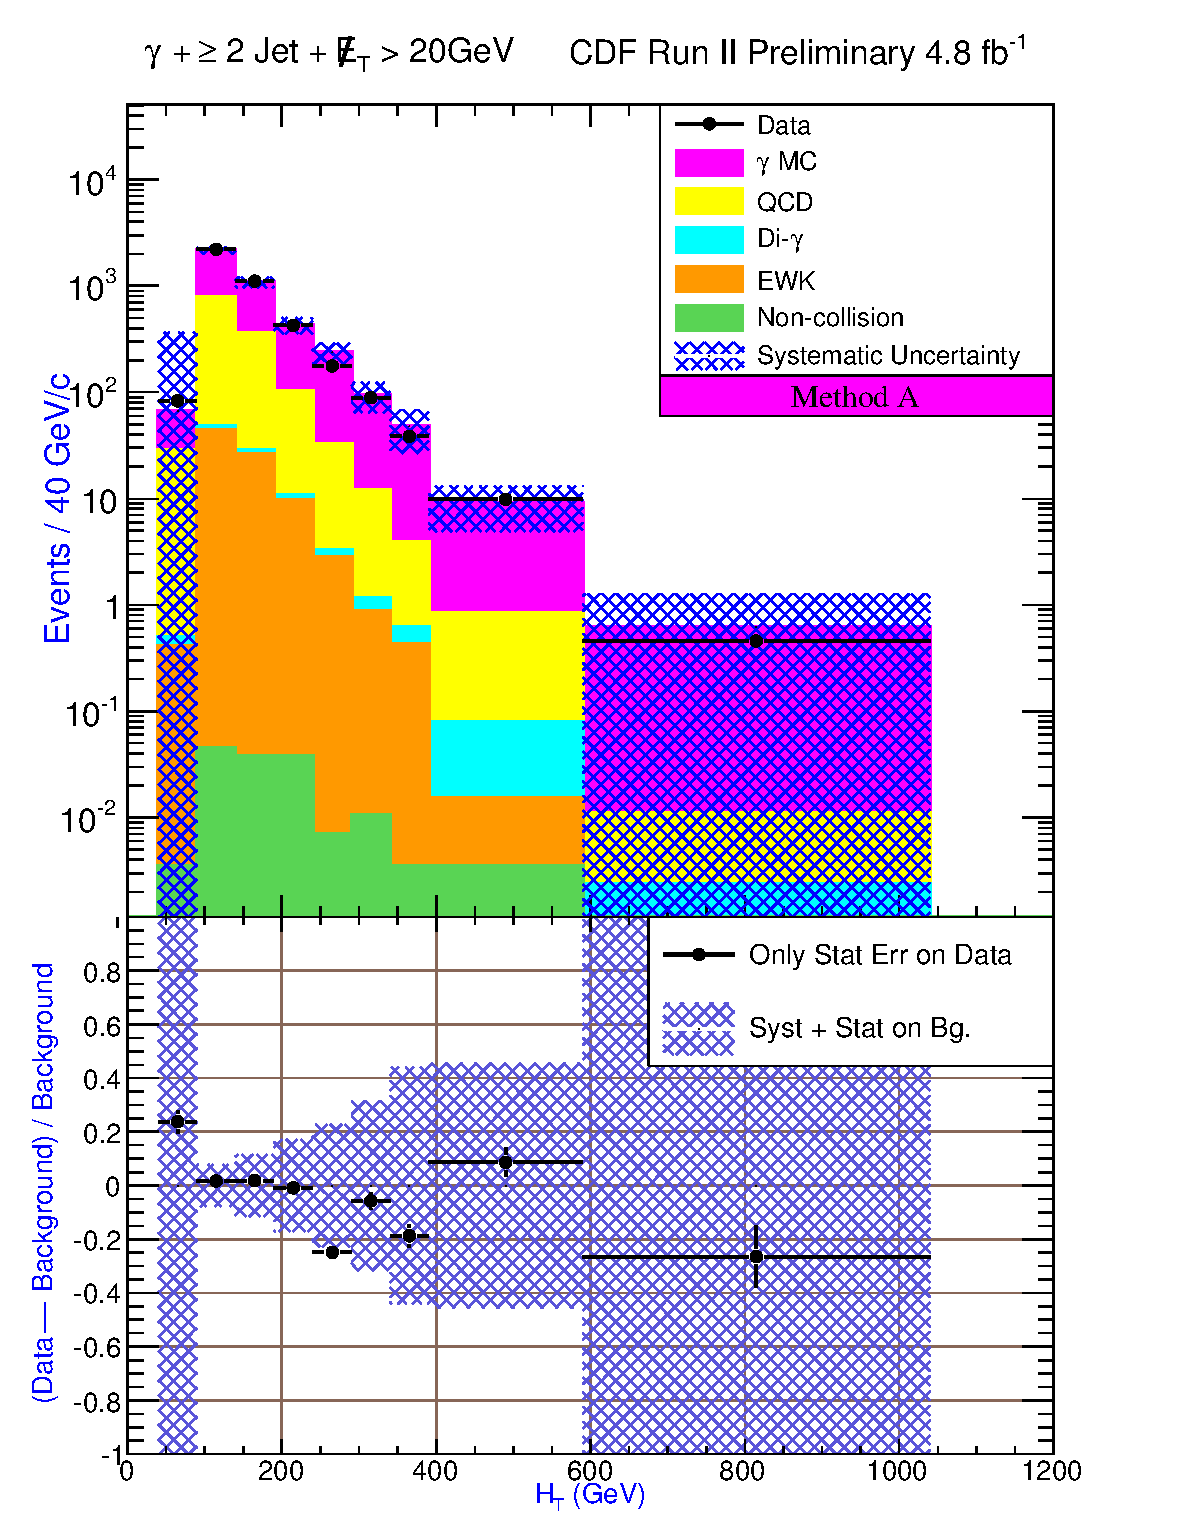
\includegraphics[keepaspectratio=true, scale=\resultsHistScale]{G30JetsMet20_MtdA_plot2_Ht.pdf}}
\subfigure[]
{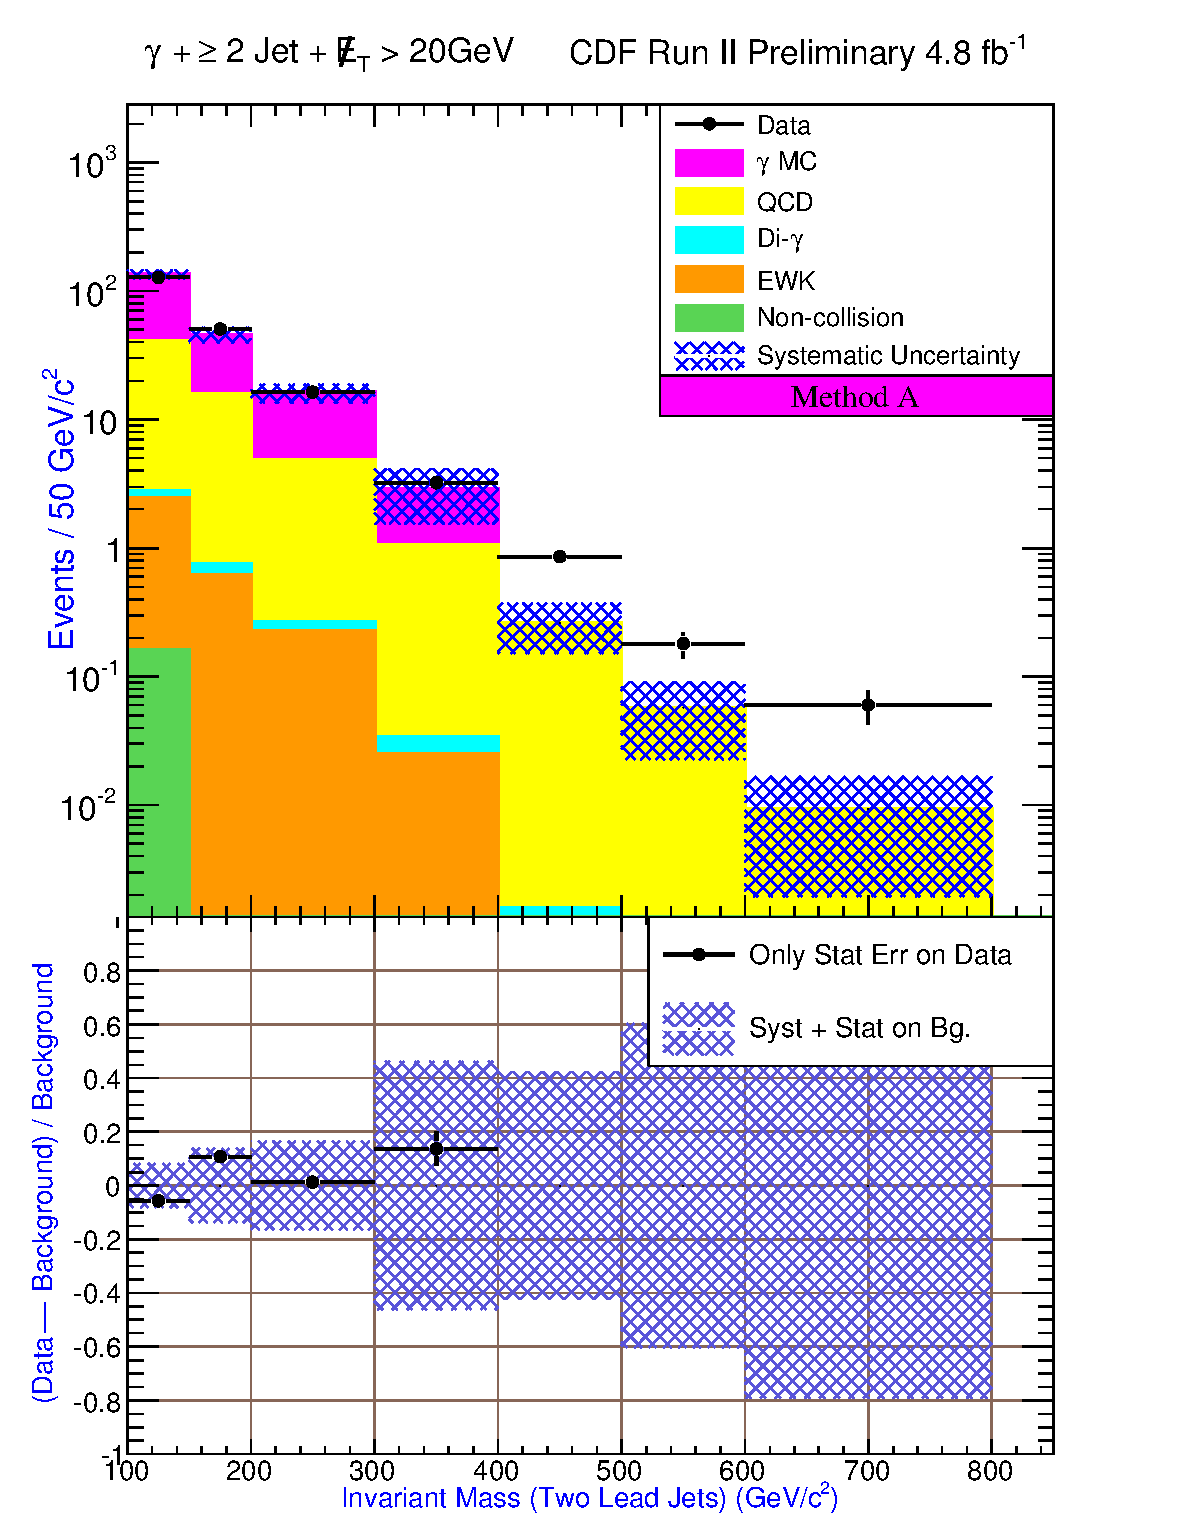
\includegraphics[keepaspectratio=true, scale=\resultsHistScale]{G30JetsMet20_MtdA_plot2_InvMass_j1j2.pdf}}
\subfigure[]
{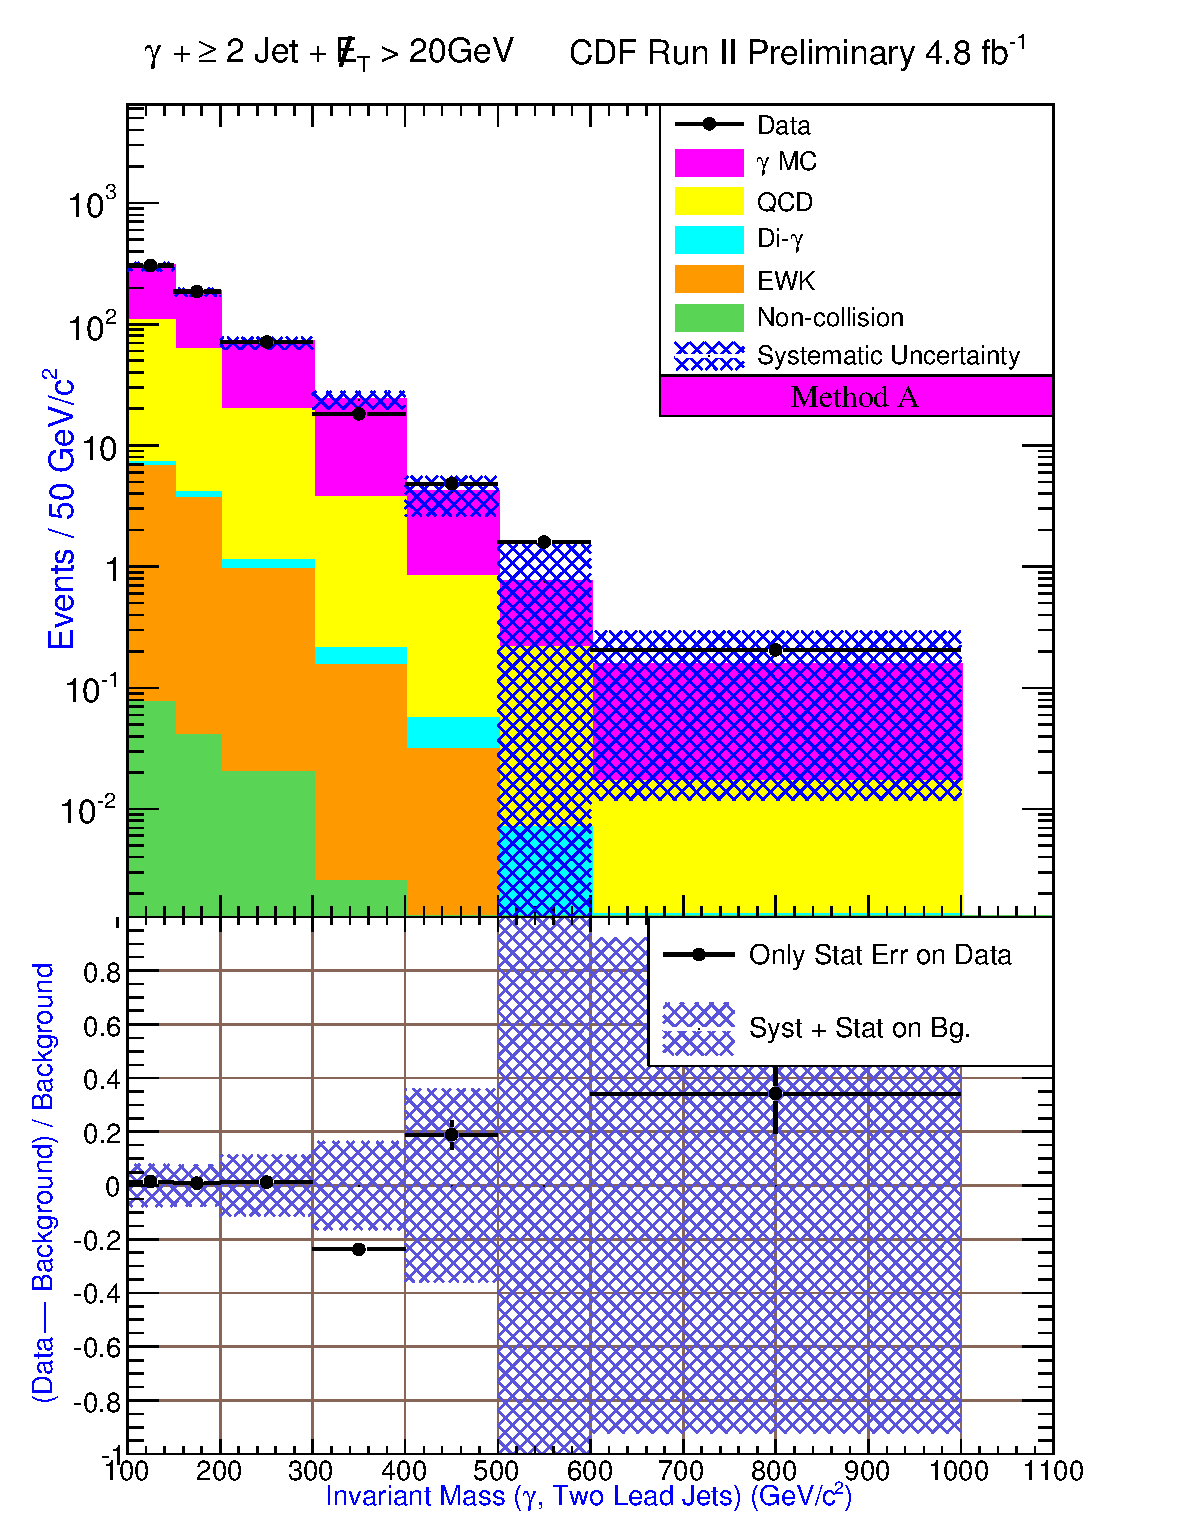
\includegraphics[keepaspectratio=true, scale=\resultsHistScale]{G30JetsMet20_MtdA_plot2_InvMass_pj1j2.pdf}}
\subfigure[]
{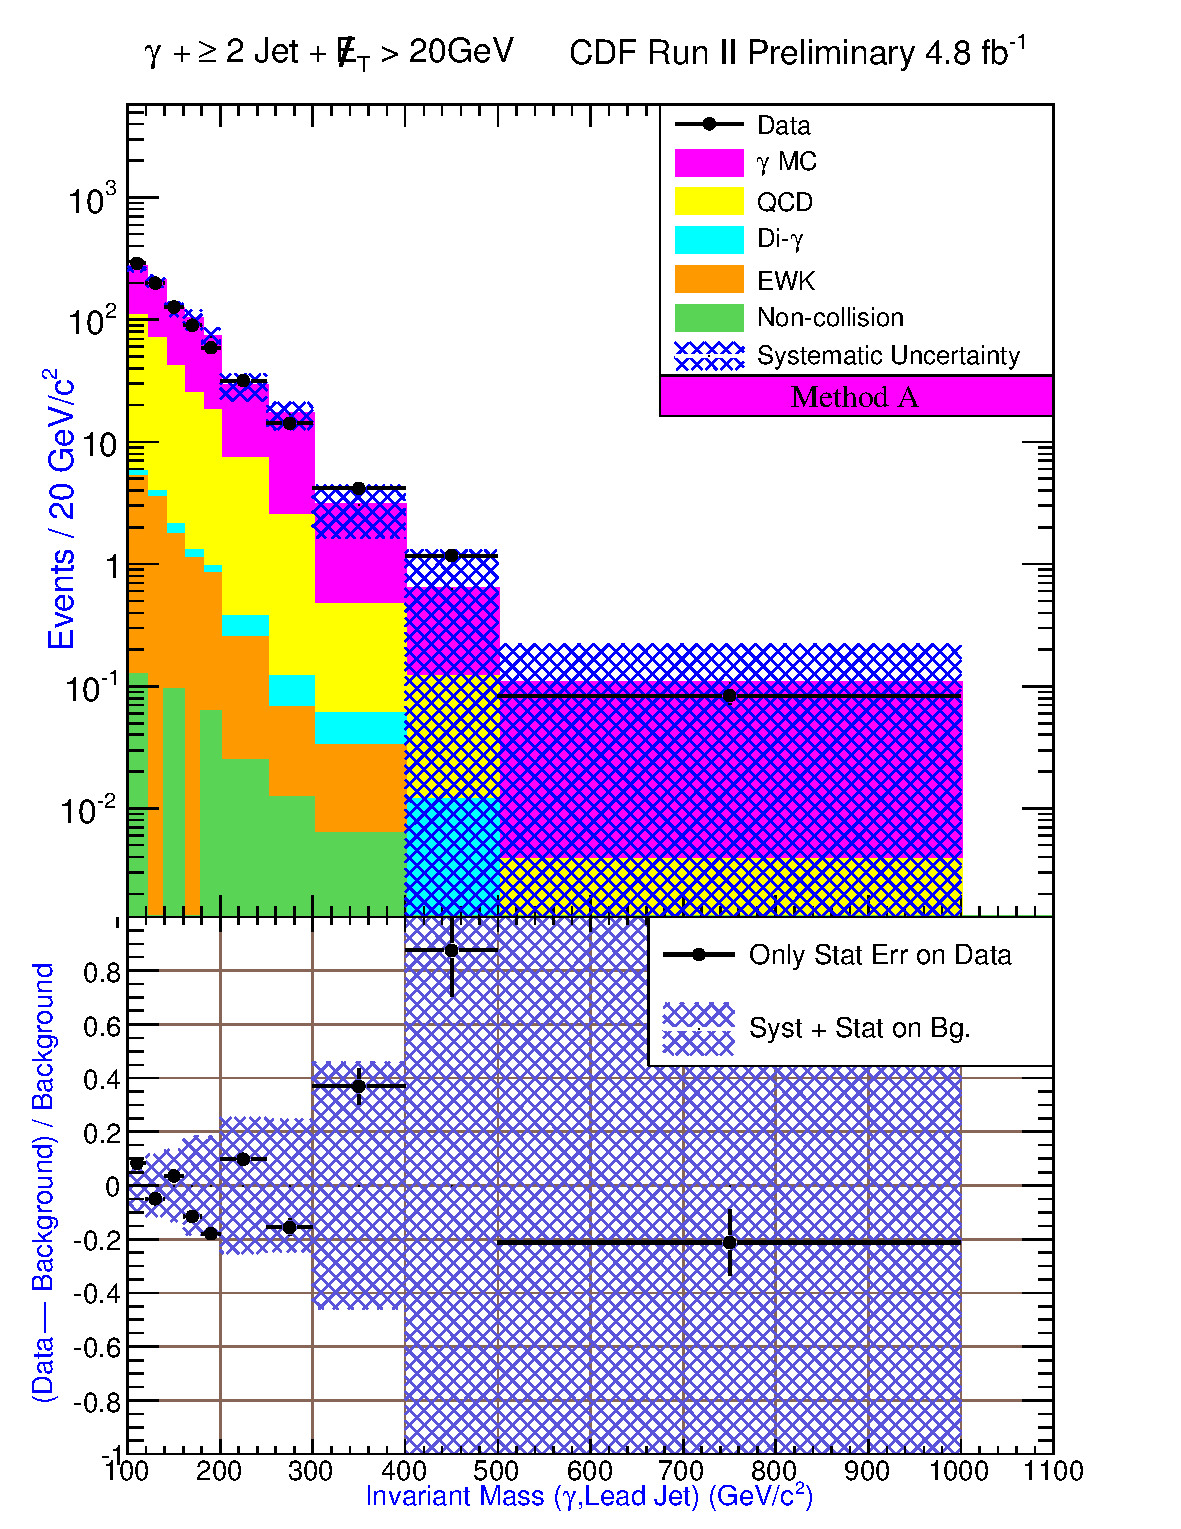
\includegraphics[keepaspectratio=true, scale=\resultsHistScale]{G30JetsMet20_MtdA_plot2_InvMass_pj1.pdf}}
\caption{Kinematic distributions of \photwojet + \met$>$~20~\etUnits events using \mbox{Method A}. The beginning of Chapter~\ref{chp:Results} provides a description of the elements in these distributions.}
\label{fig:pjMetSetThree}
\end{figure*}
\clearpage

\begin{figure*}[p]
\centering
\subfigure[]
{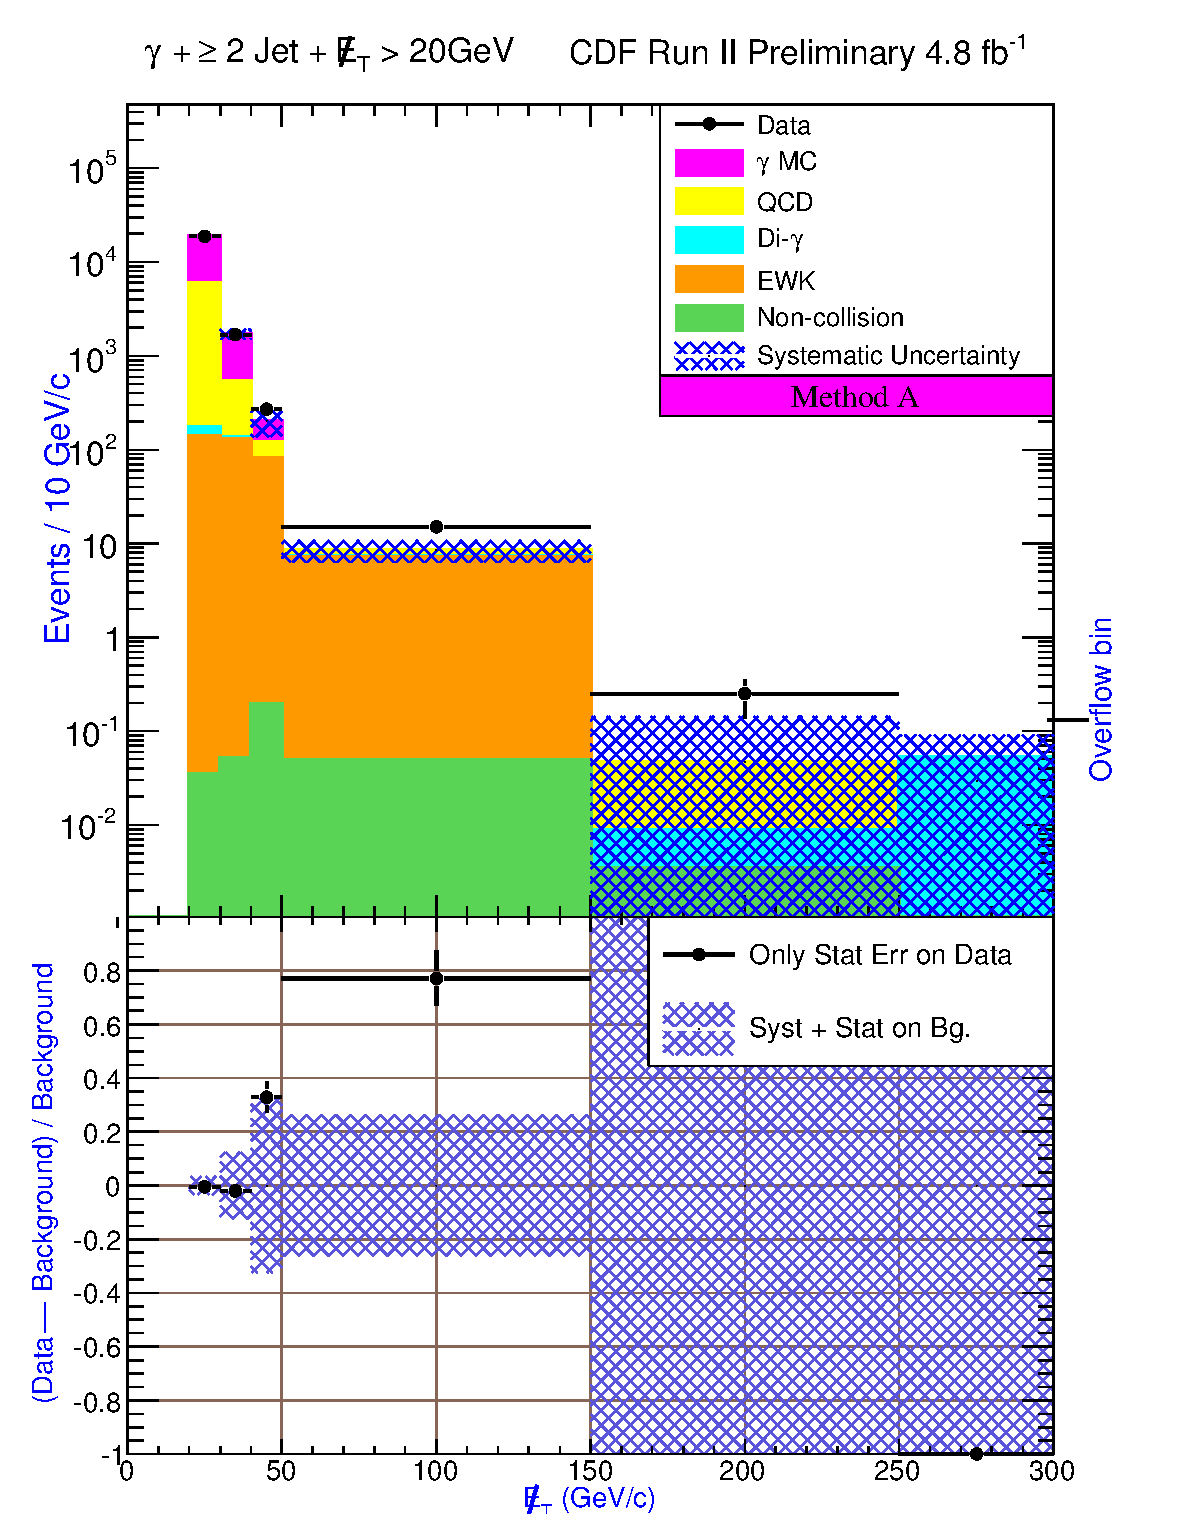
\includegraphics[keepaspectratio=true, scale=0.7]{G30JetsMet20_MtdA_plot2_Met.pdf}}
\caption{Kinematic distributions of \photwojet + \met$>$~20~\etUnits events using \mbox{Method A}. The beginning of Chapter~\ref{chp:Results} provides a description of the elements in these distributions.}
\label{fig:pjMetSetFour}
\end{figure*}



\clearpage
%%%%%%%%%%%%%%%%%%%%%%%%%%%%%%%%%%%% METHOD B: G30 JETS

\begin{figure*}[h!]
 \centering
\subfigure[]
{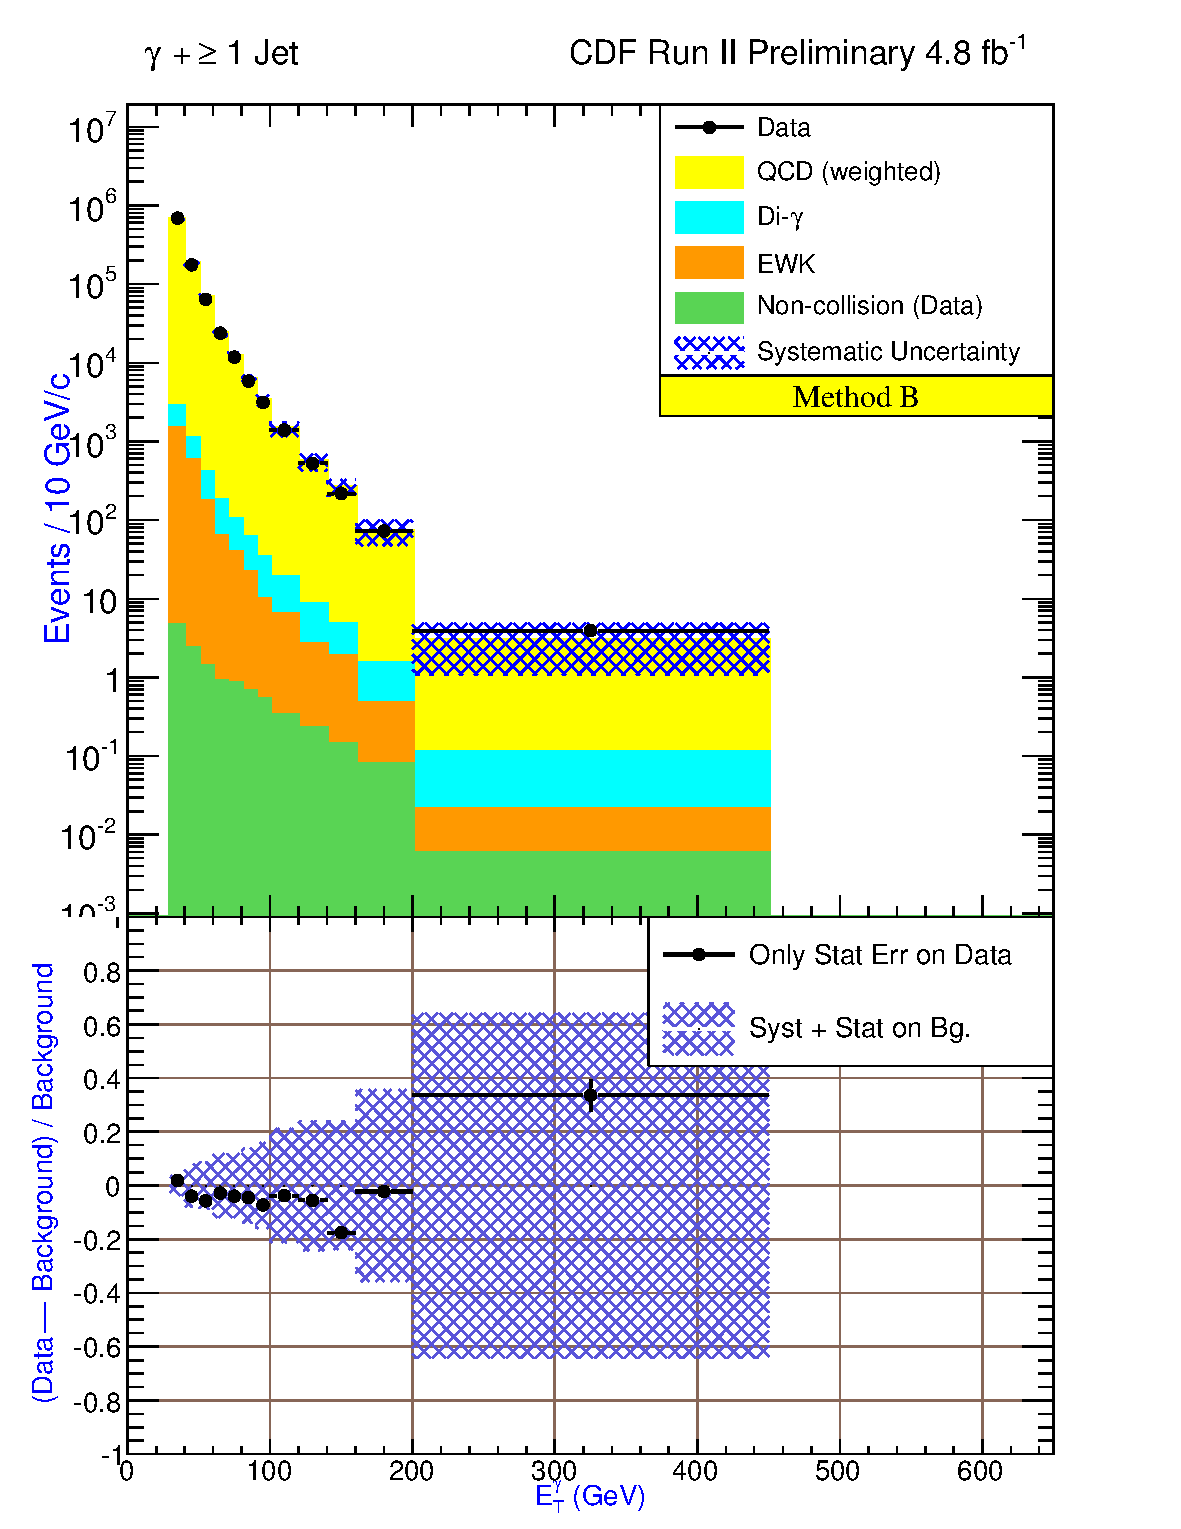
\includegraphics[keepaspectratio=true, scale=\resultsHistScale]{G30Jets_MtdB_plot1_Et_pho.pdf}}
\subfigure[]
{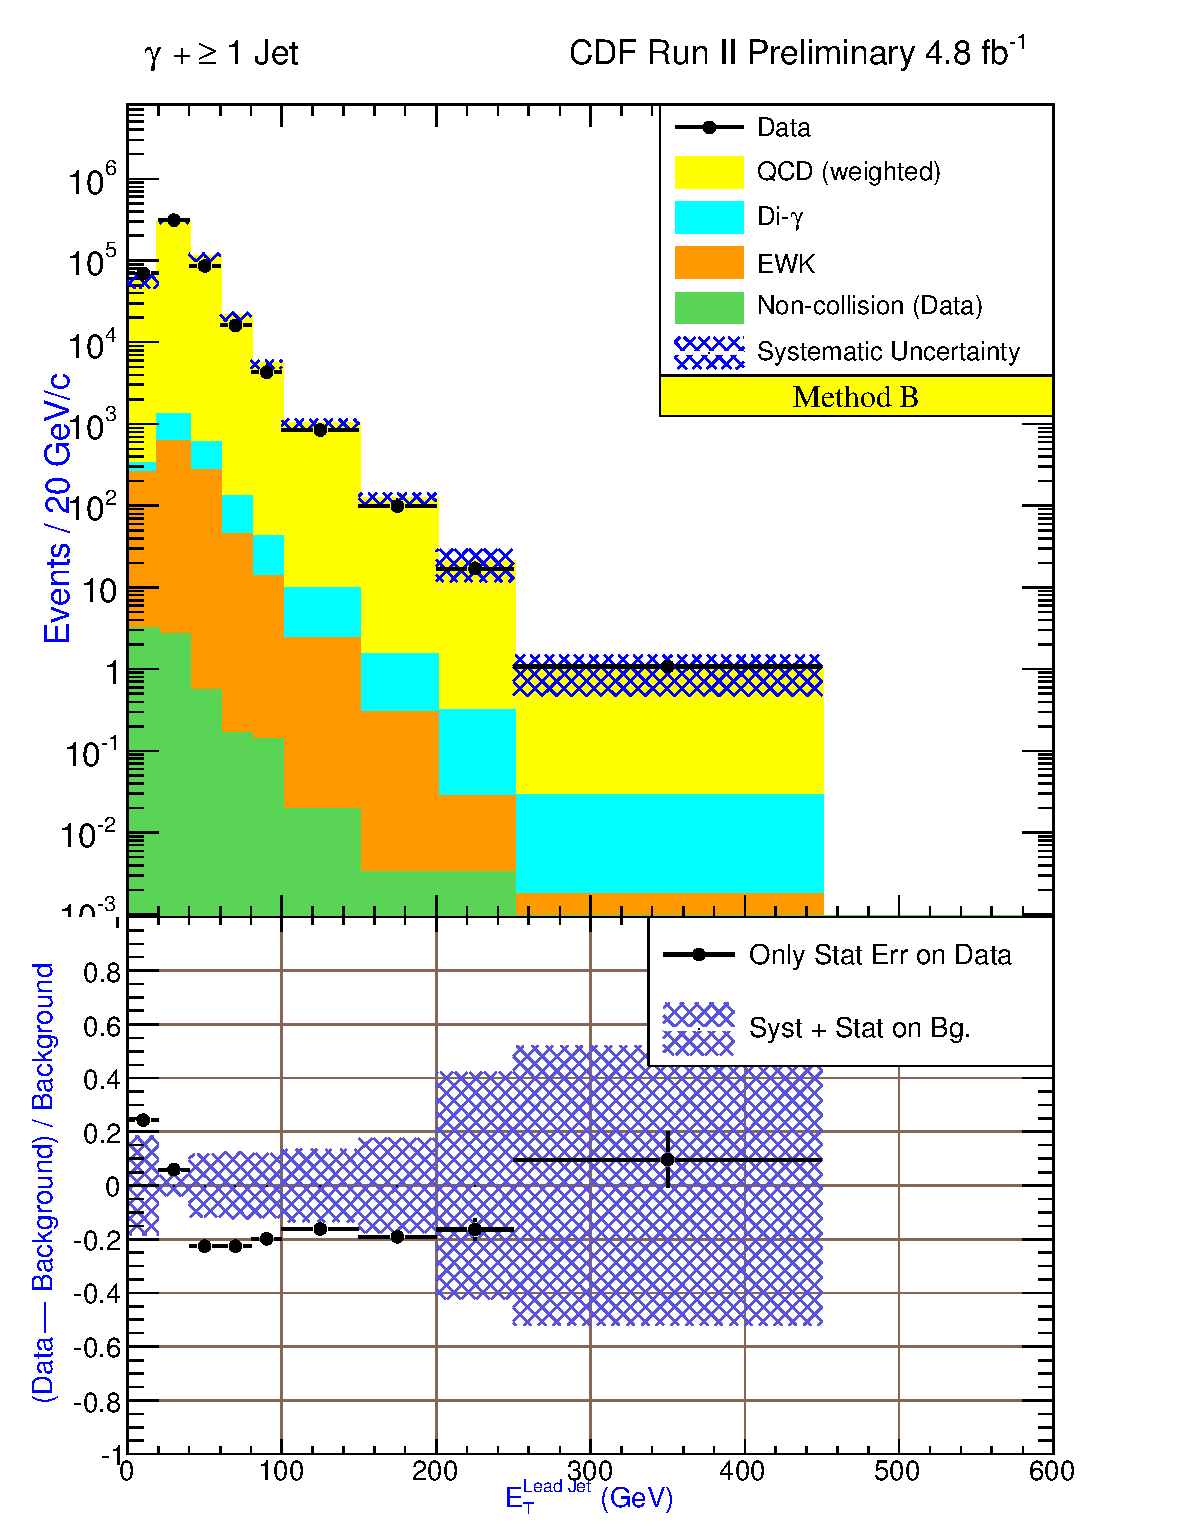
\includegraphics[keepaspectratio=true, scale=\resultsHistScale]{G30Jets_MtdB_plot1_Et_j1.pdf}}
\subfigure[]
{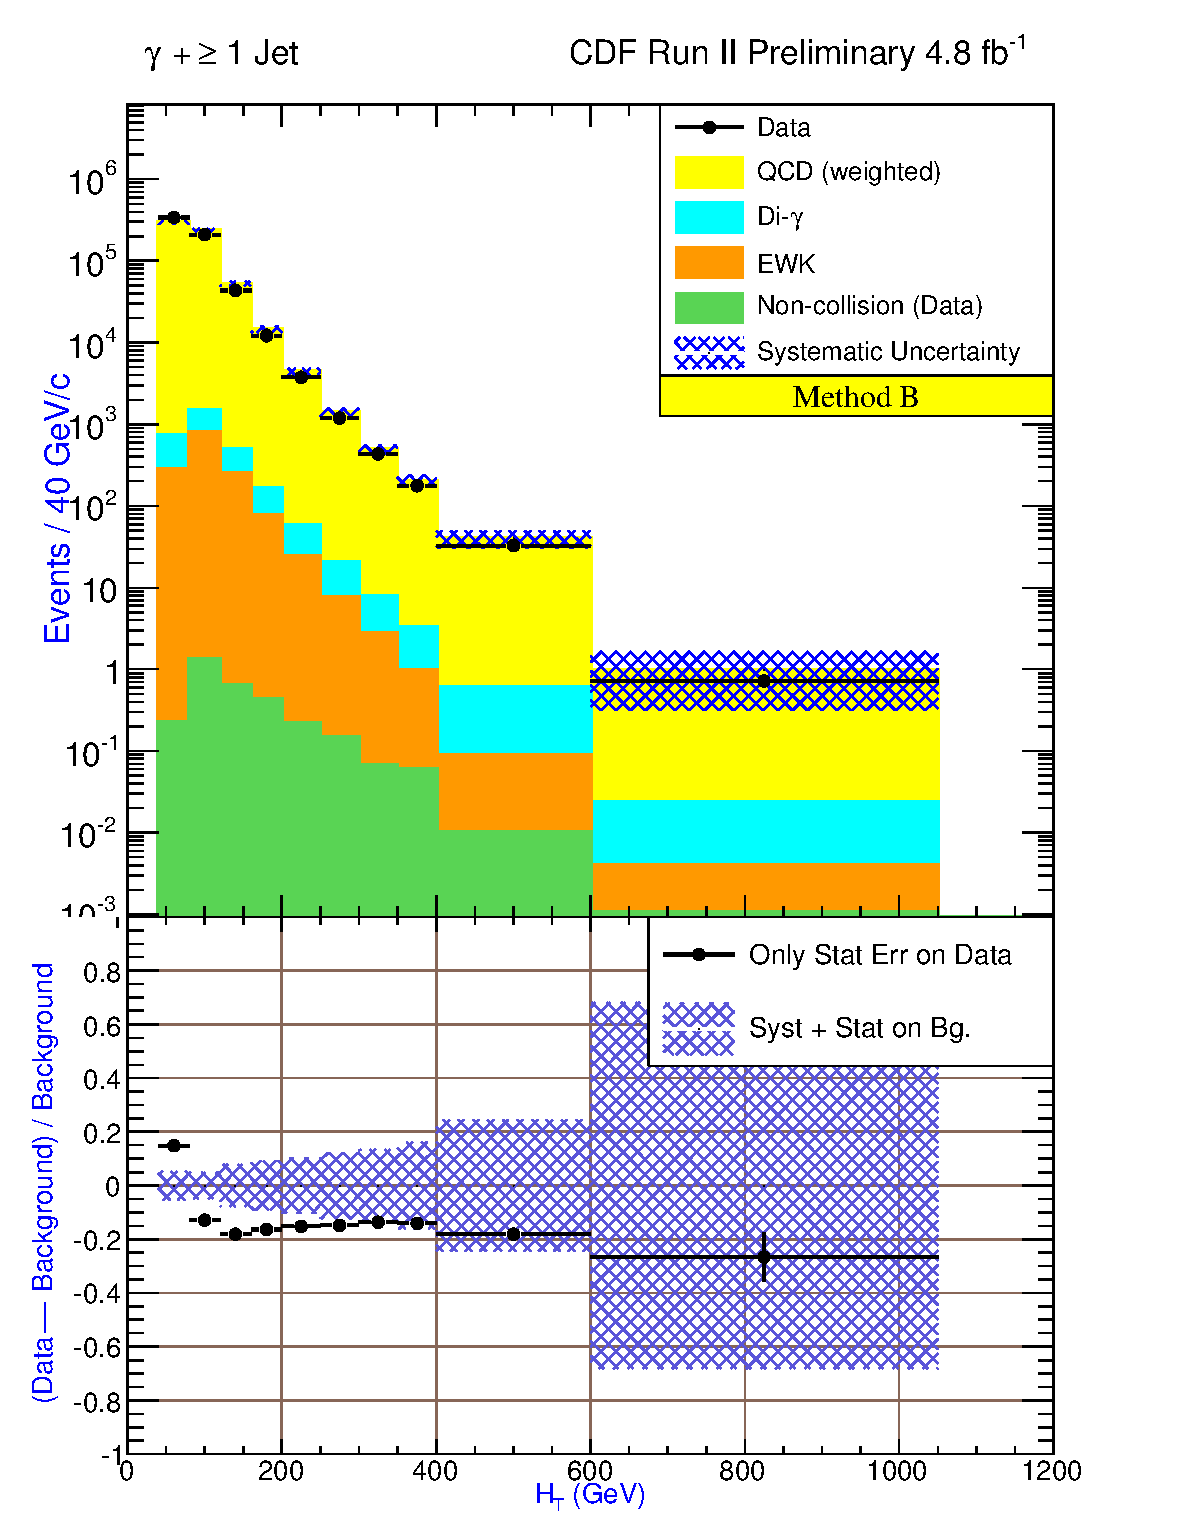
\includegraphics[keepaspectratio=true, scale=\resultsHistScale]{G30Jets_MtdB_plot1_Ht.pdf}}
\subfigure[]
{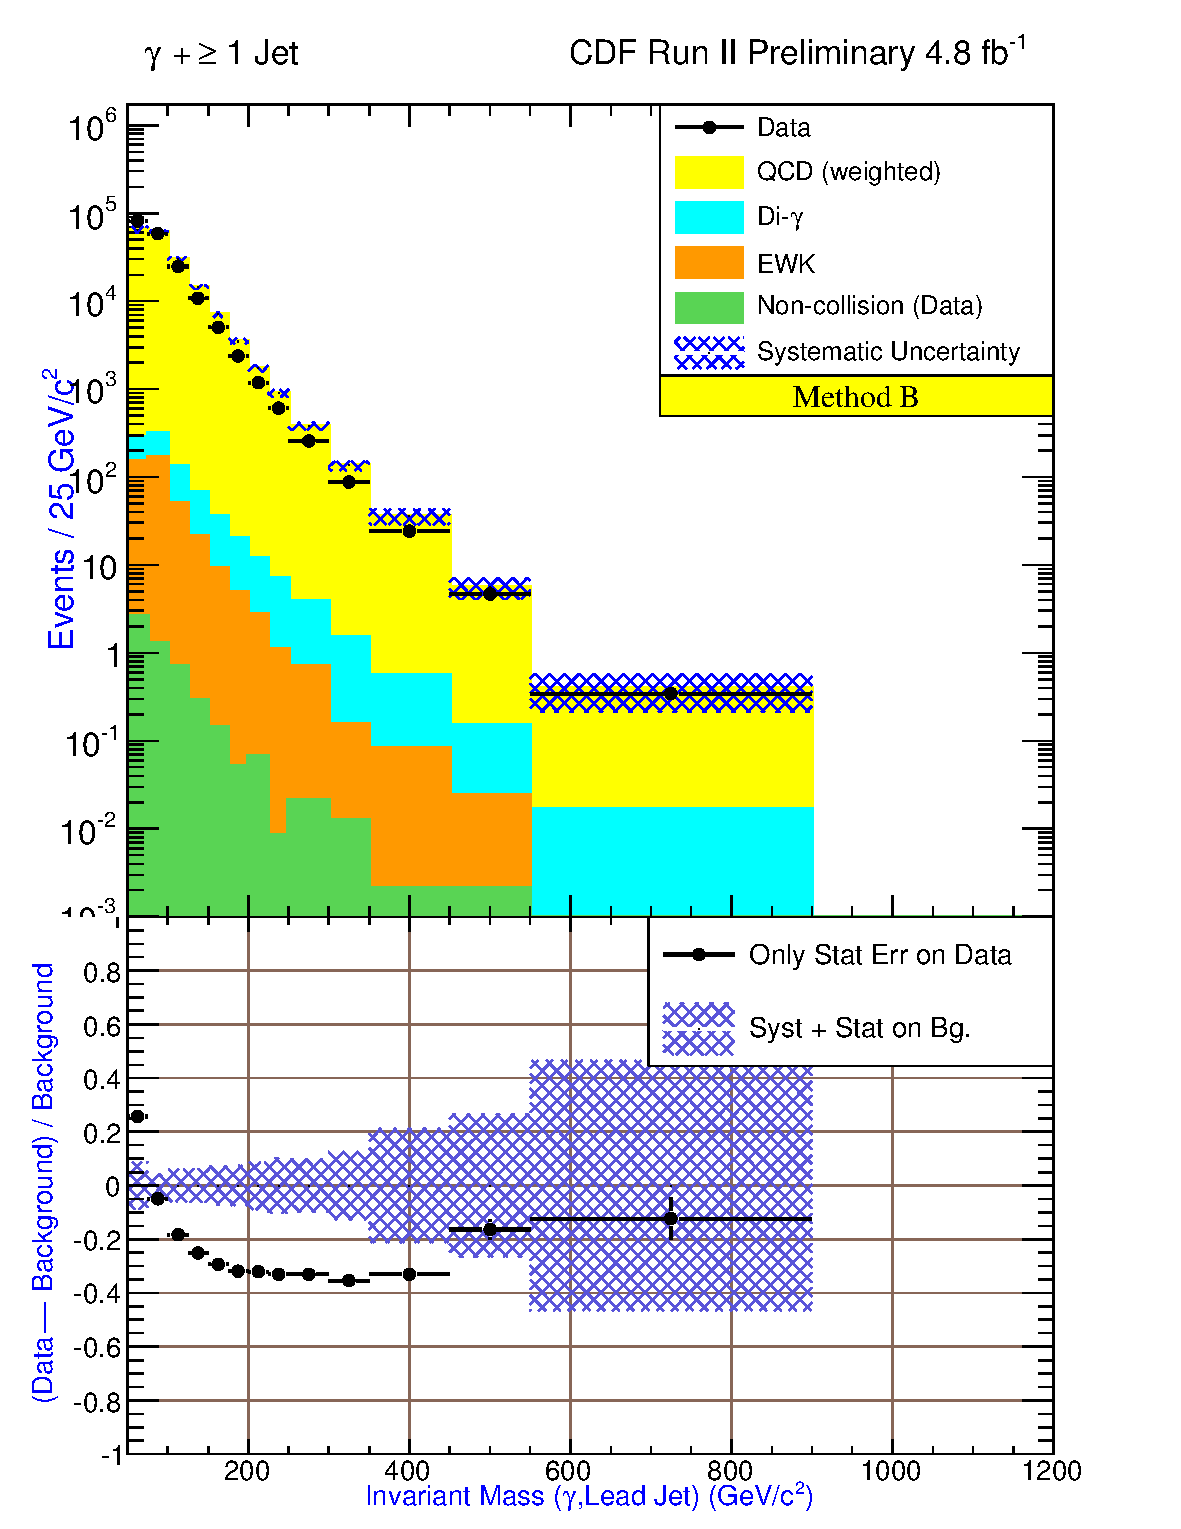
\includegraphics[keepaspectratio=true, scale=\resultsHistScale]{G30Jets_MtdB_plot1_InvMass_pj1.pdf}
\label{fig:pjMtdBSetOne:Mass_pj1}
}
\caption{Kinematic distributions of \phoonejet events using \mbox{Method B}. The beginning of Chapter~\ref{chp:Results} provides a description of the elements in these distributions.}
\label{fig:pjMtdBSetOne}
\end{figure*}
\clearpage

\begin{figure*}[h!]
\centering
\subfigure[]
{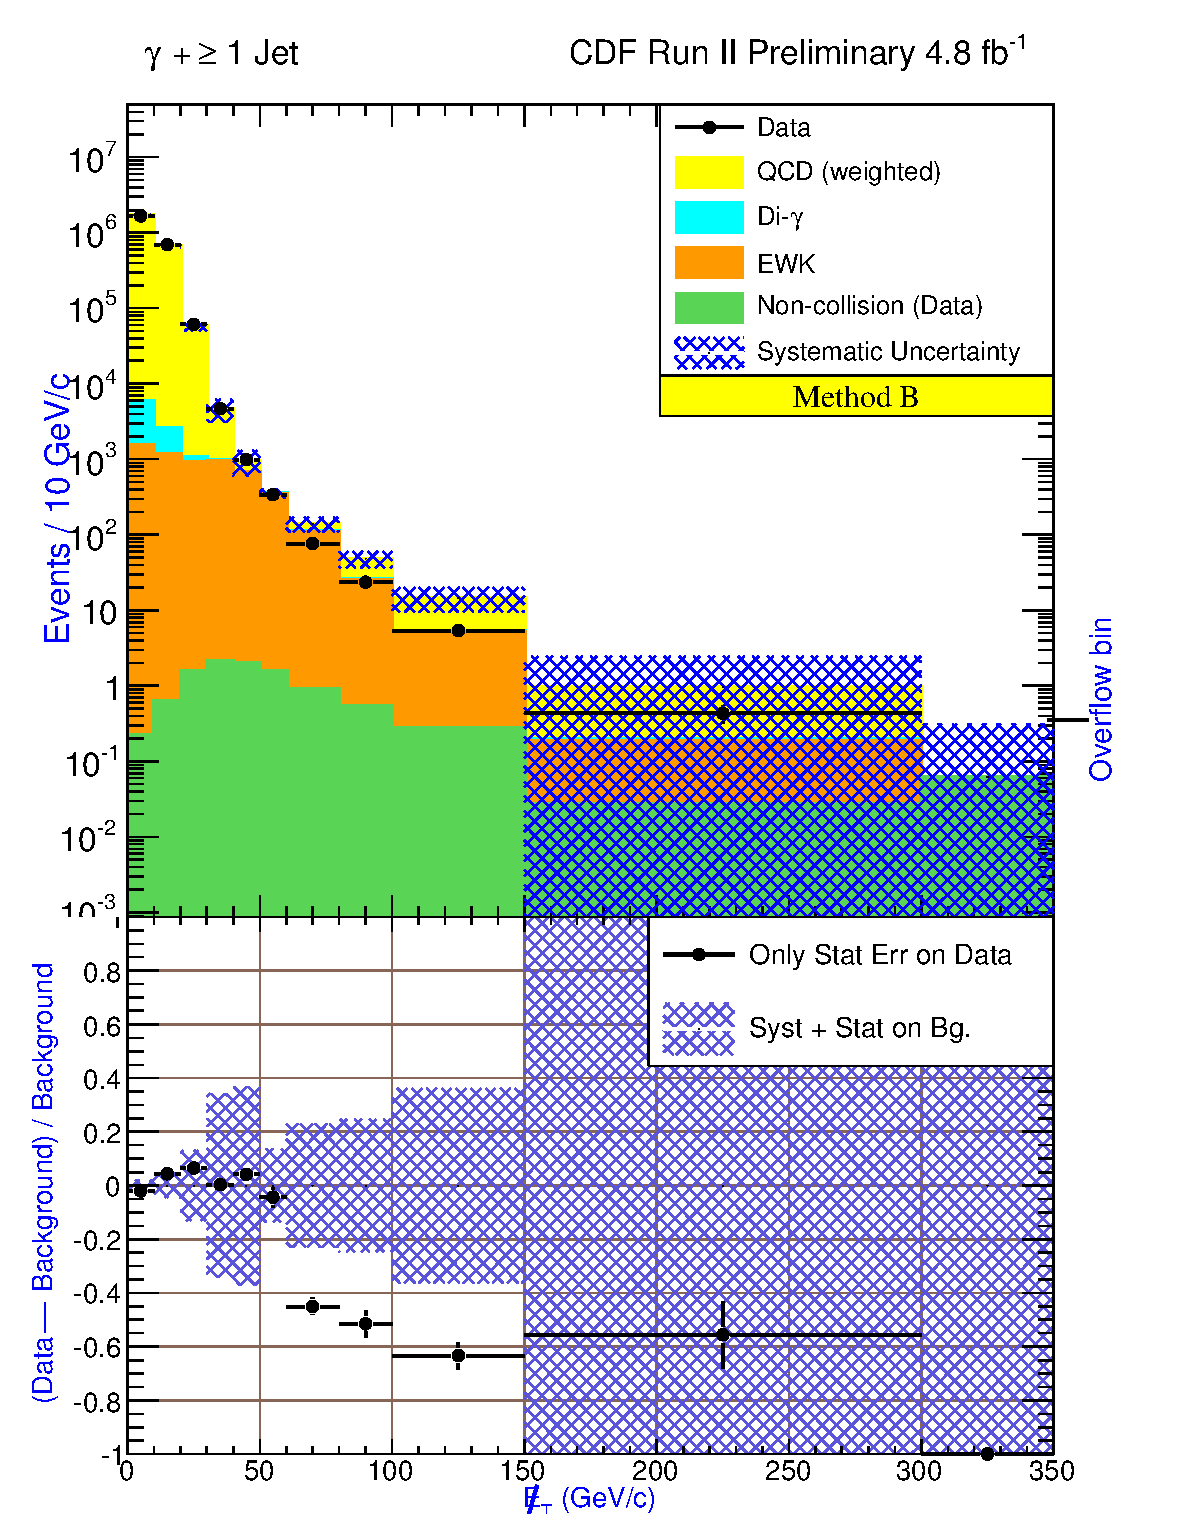
\includegraphics[keepaspectratio=true, scale=\resultsHistScale]{G30Jets_MtdB_plot1_Met.pdf}}
\subfigure[]
{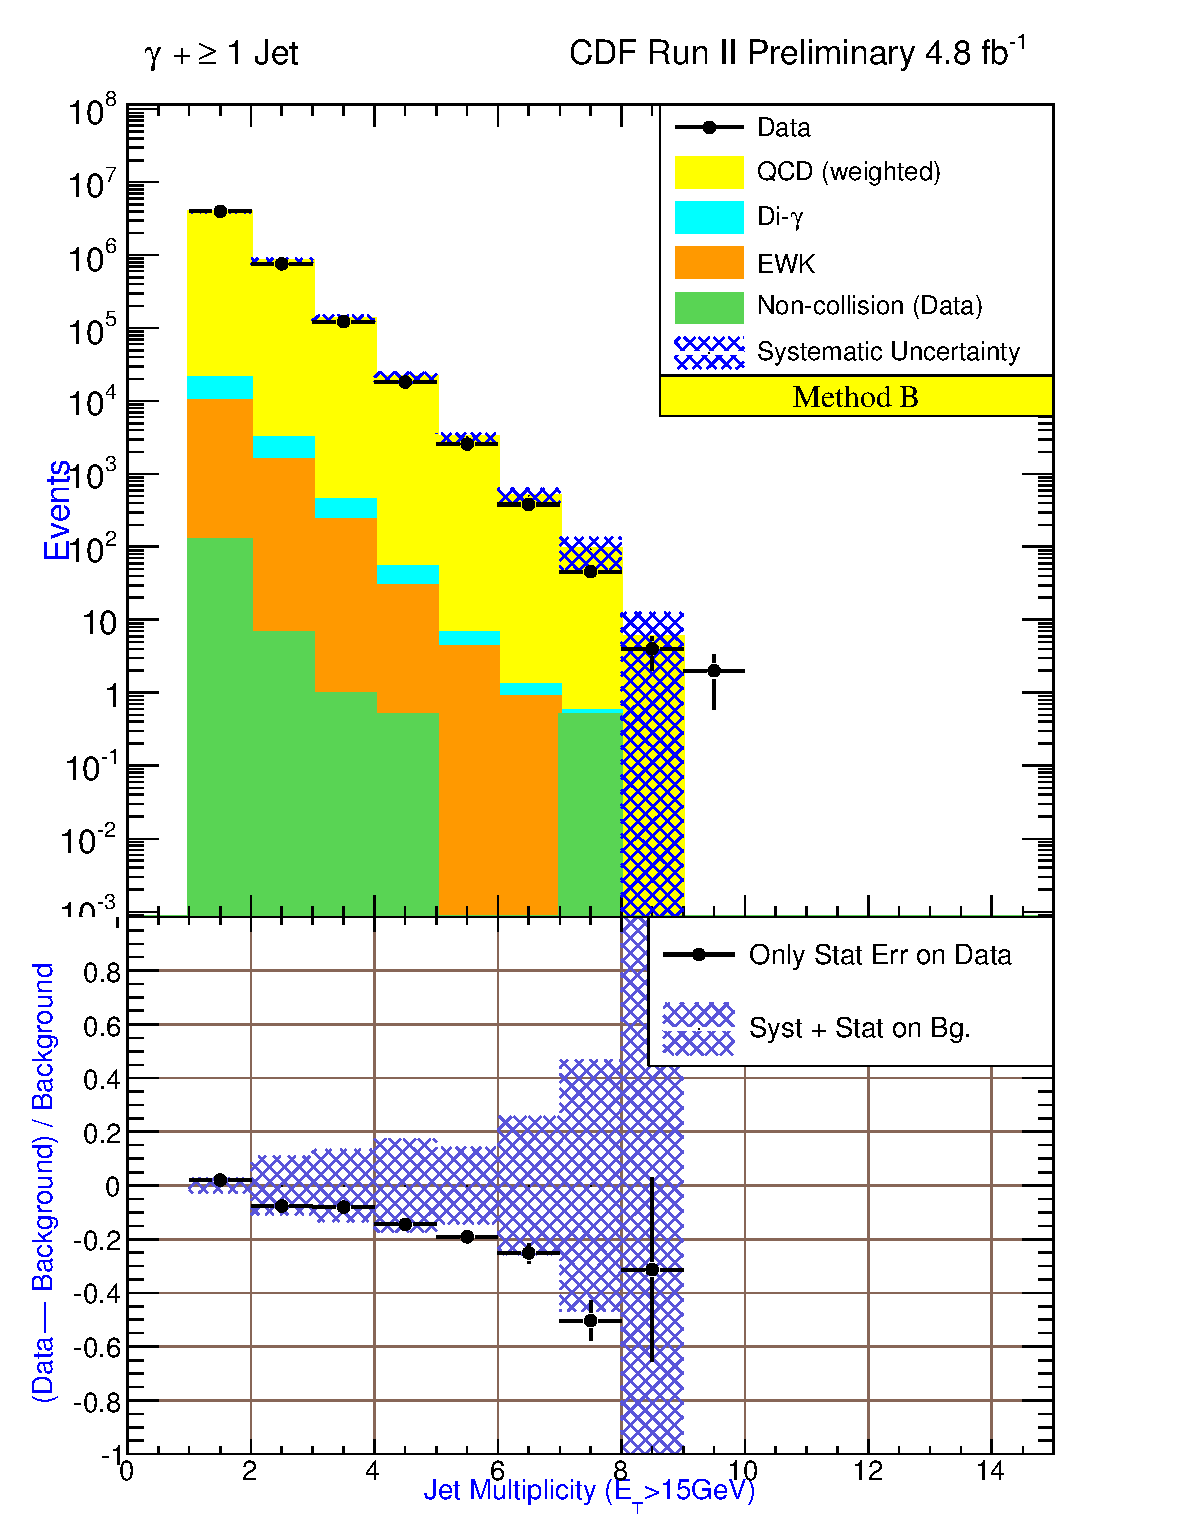
\includegraphics[keepaspectratio=true, scale=\resultsHistScale]{G30Jets_MtdB_plot1_NJet.pdf}}
\subfigure[]
{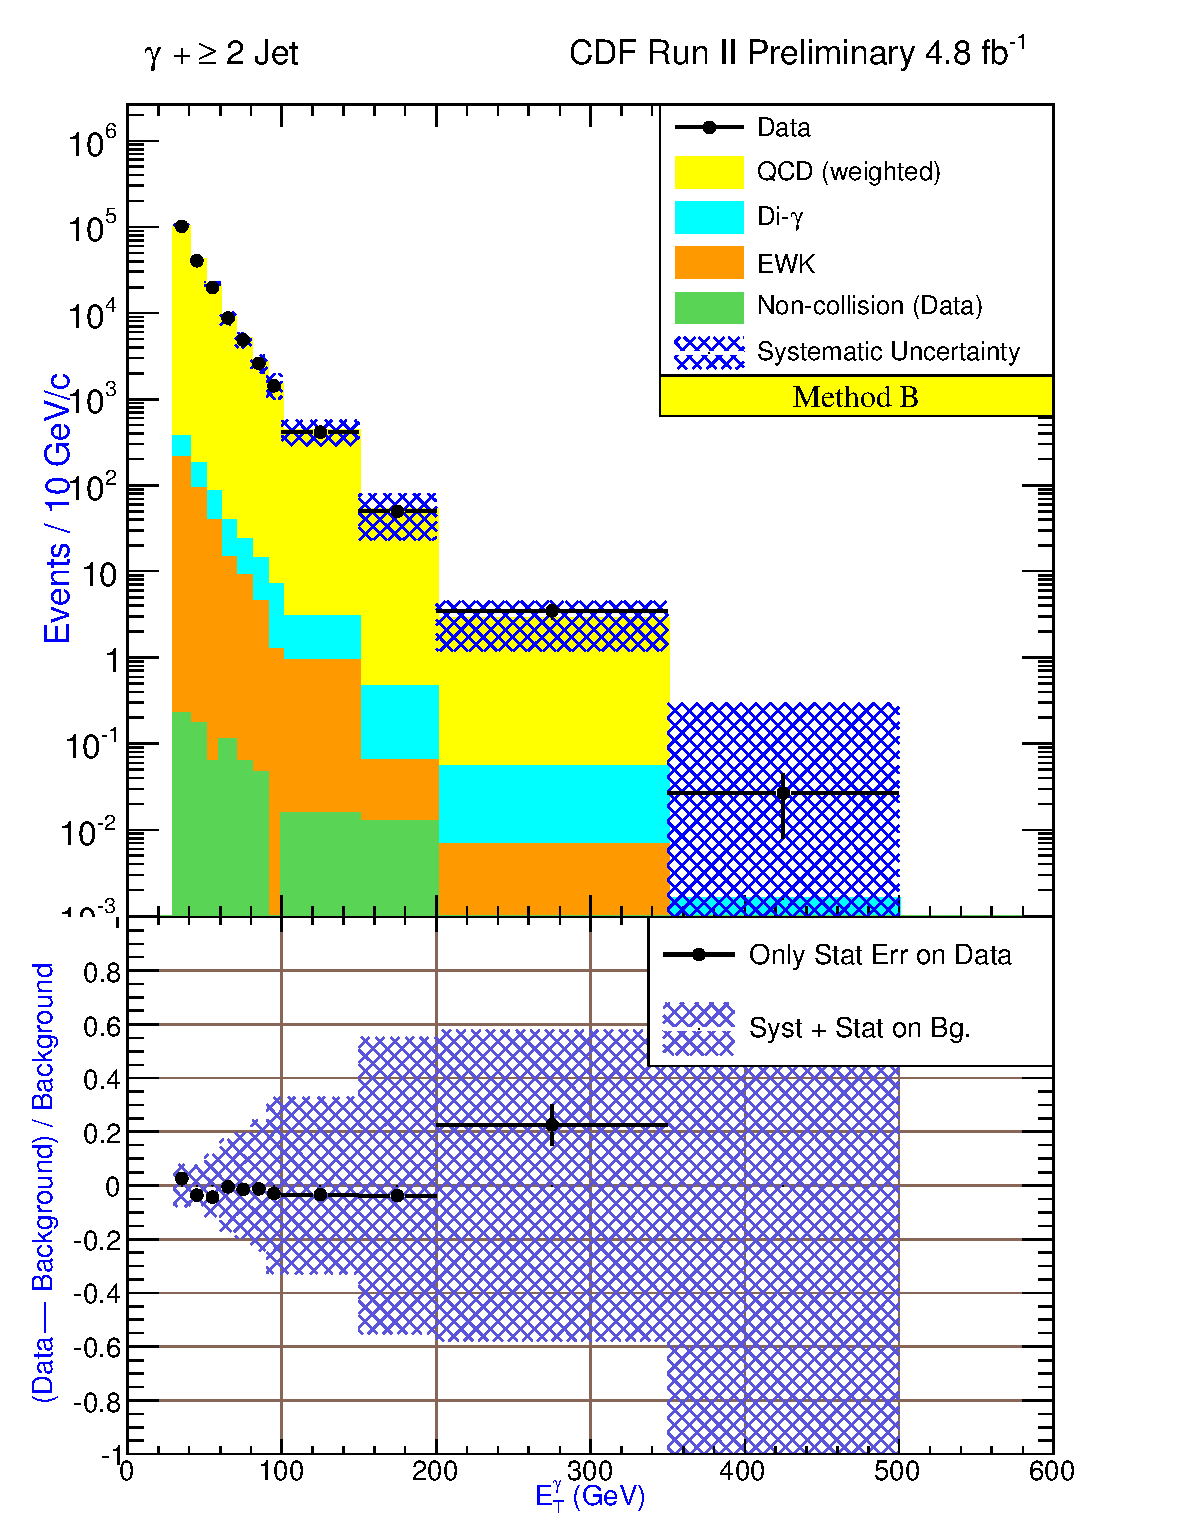
\includegraphics[keepaspectratio=true, scale=\resultsHistScale]{G30Jets_MtdB_plot2_Et_pho.pdf}}
\subfigure[]
{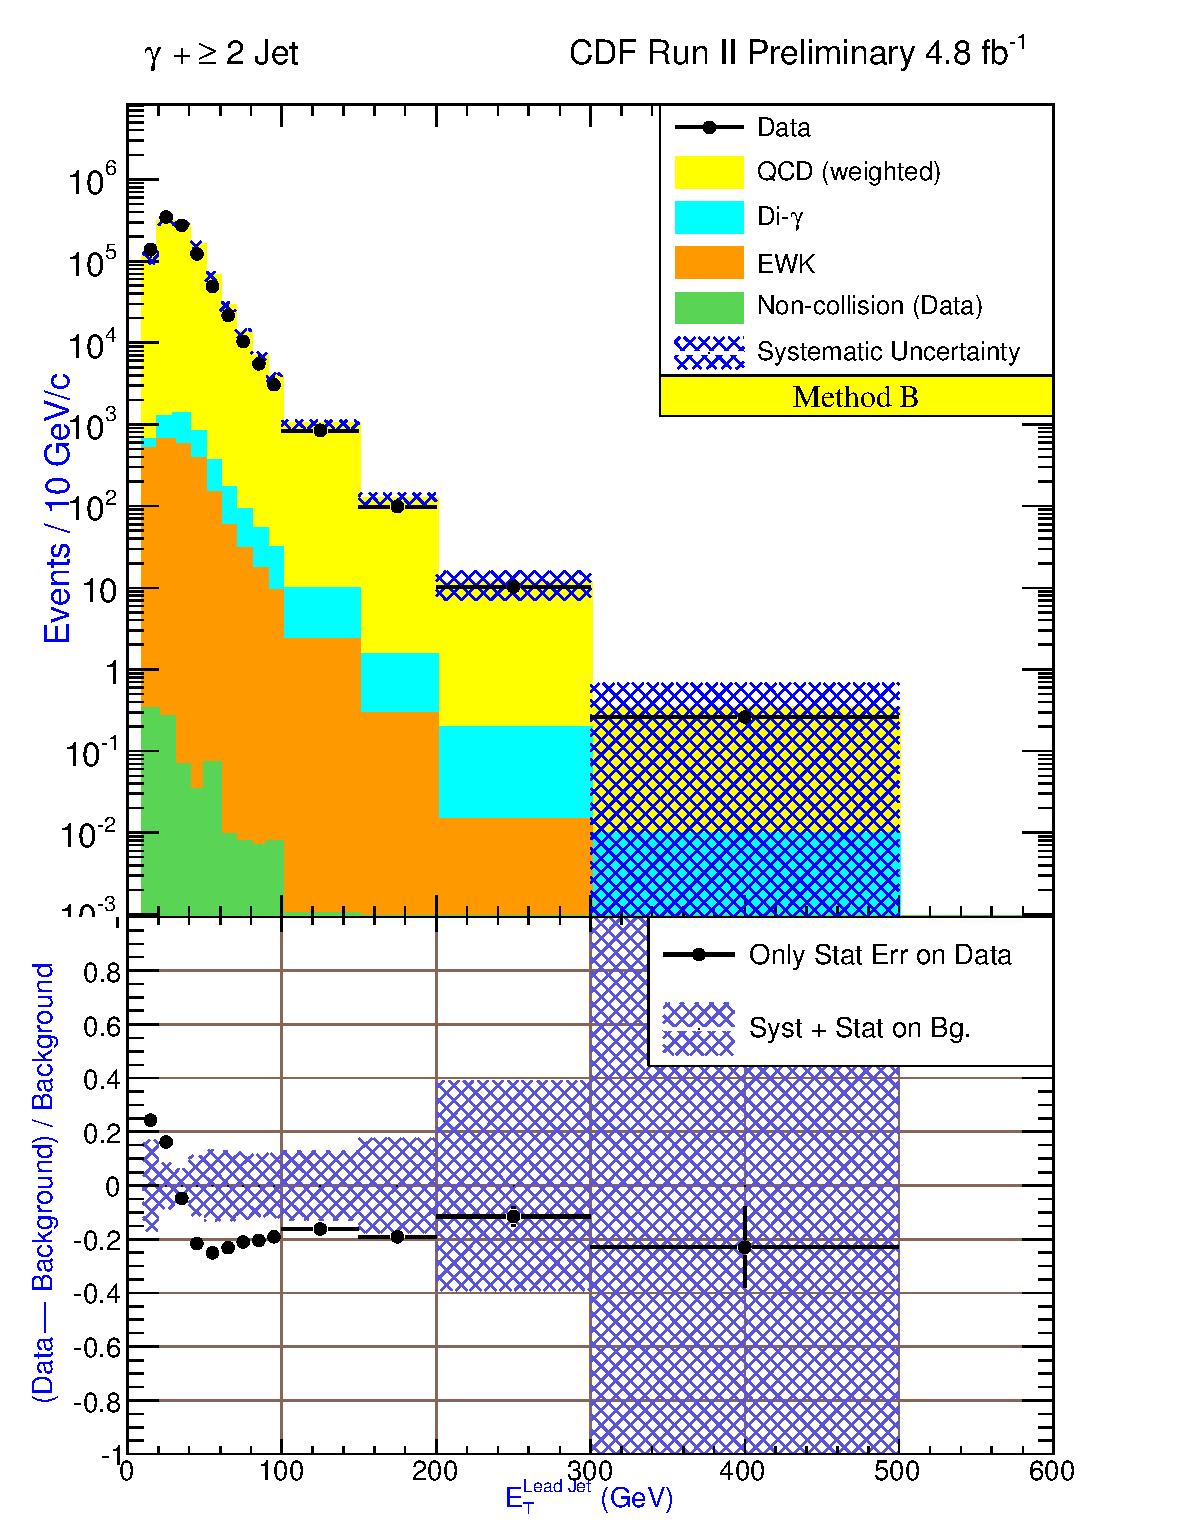
\includegraphics[keepaspectratio=true, scale=\resultsHistScale]{G30Jets_MtdB_plot2_Et_j1.pdf}}
\caption{Kinematic distributions of \phoonejet and \photwojet events using \mbox{Method B}. The beginning of Chapter~\ref{chp:Results} provides a description of the elements in these distributions.}
\label{fig:pjMtdBSetTwo}
\end{figure*}
\clearpage

\begin{figure*}[h!]
\centering
\subfigure[]
{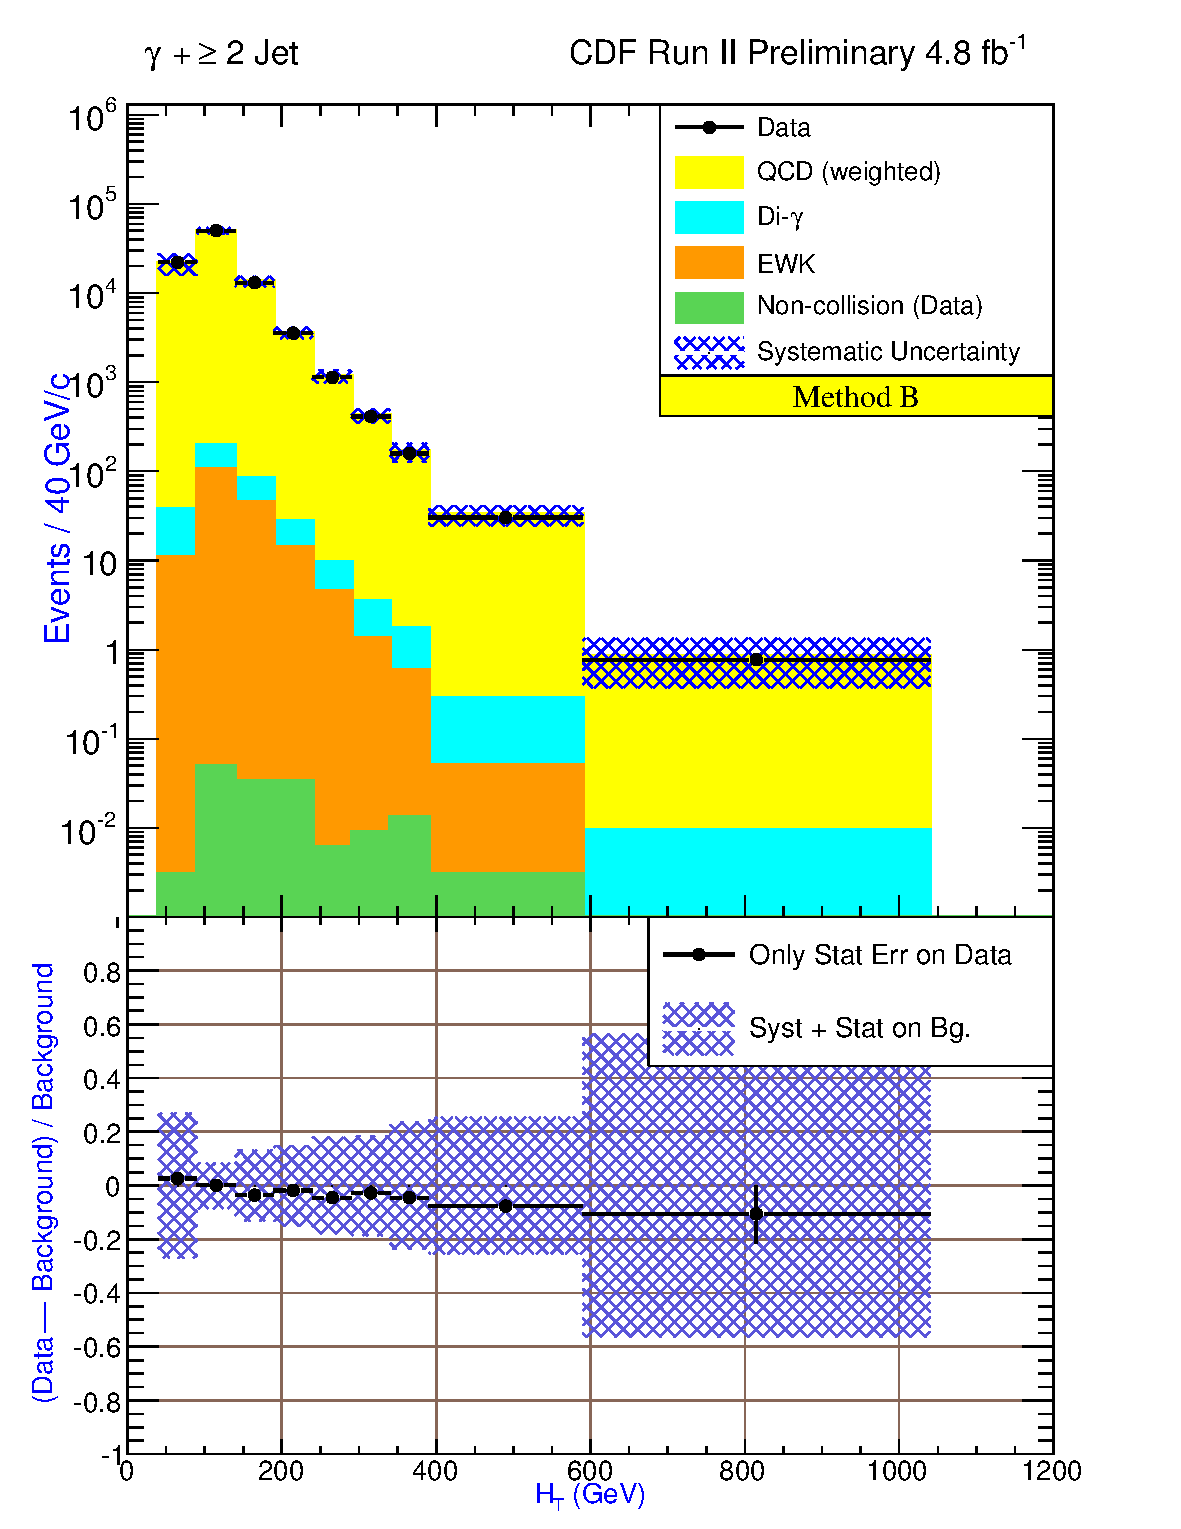
\includegraphics[keepaspectratio=true, scale=\resultsHistScale]{G30Jets_MtdB_plot2_Ht.pdf}}
\subfigure[]
{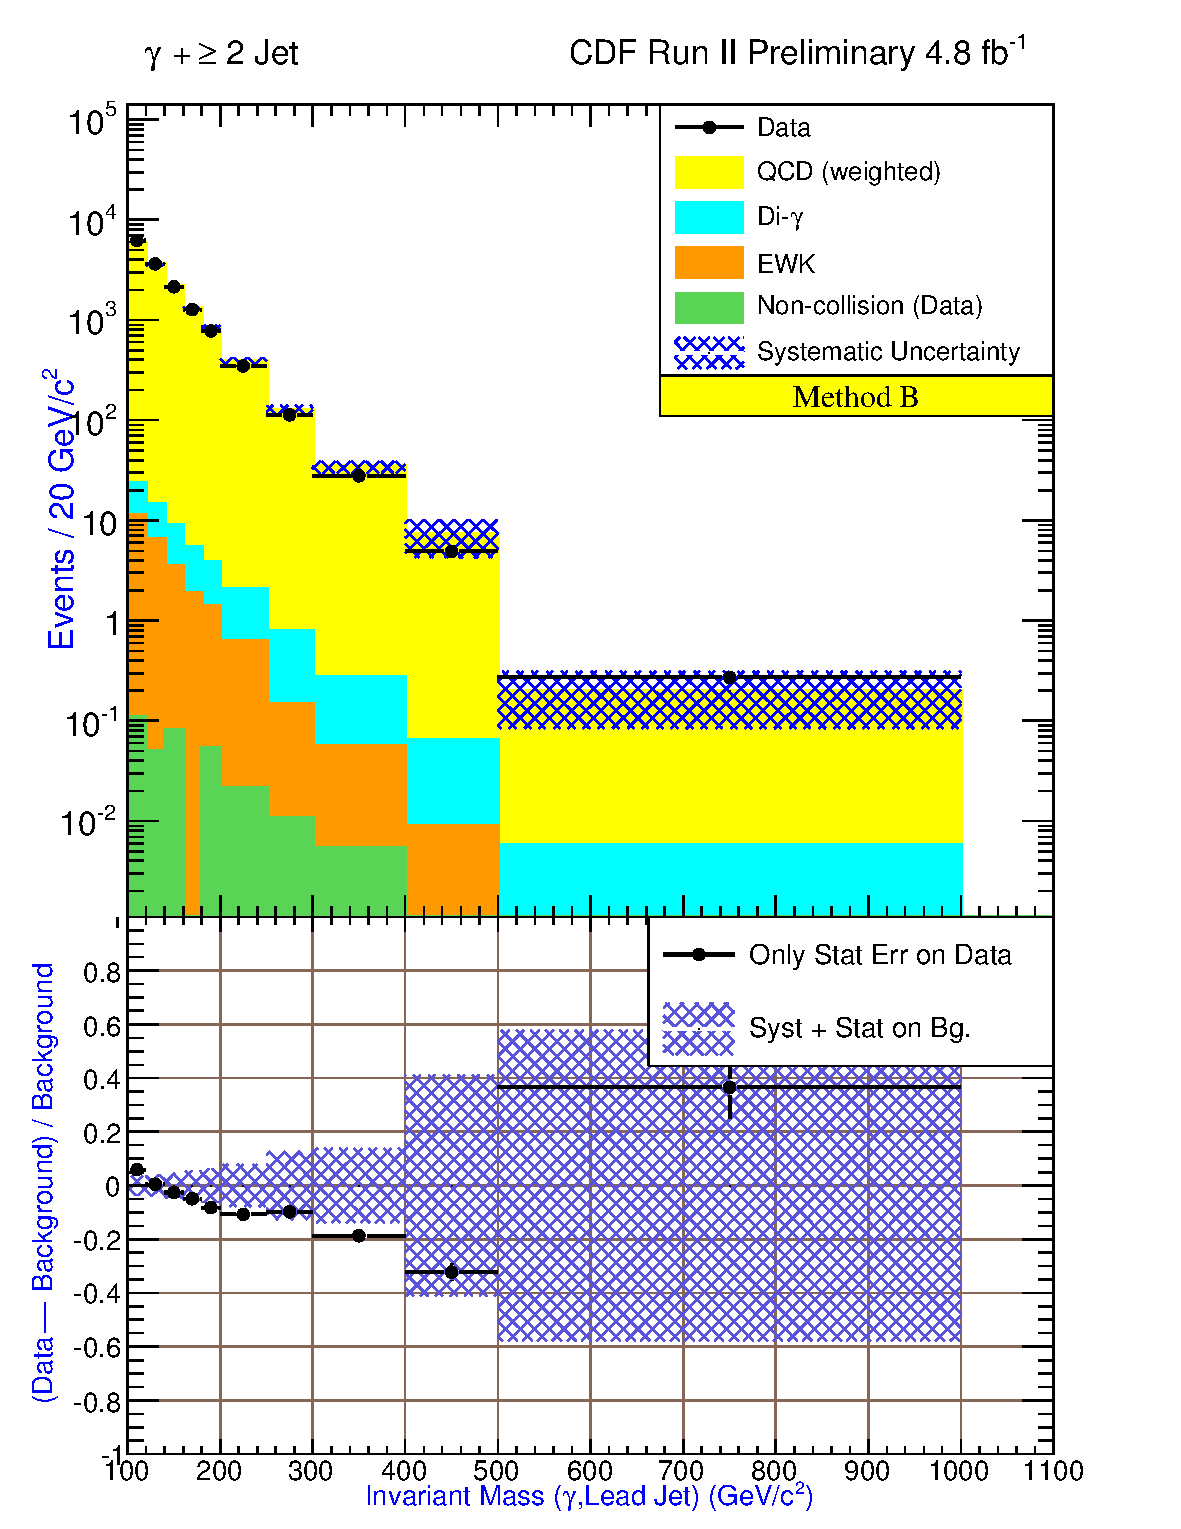
\includegraphics[keepaspectratio=true, scale=\resultsHistScale]{G30Jets_MtdB_plot2_InvMass_pj1.pdf}}
\subfigure[]
{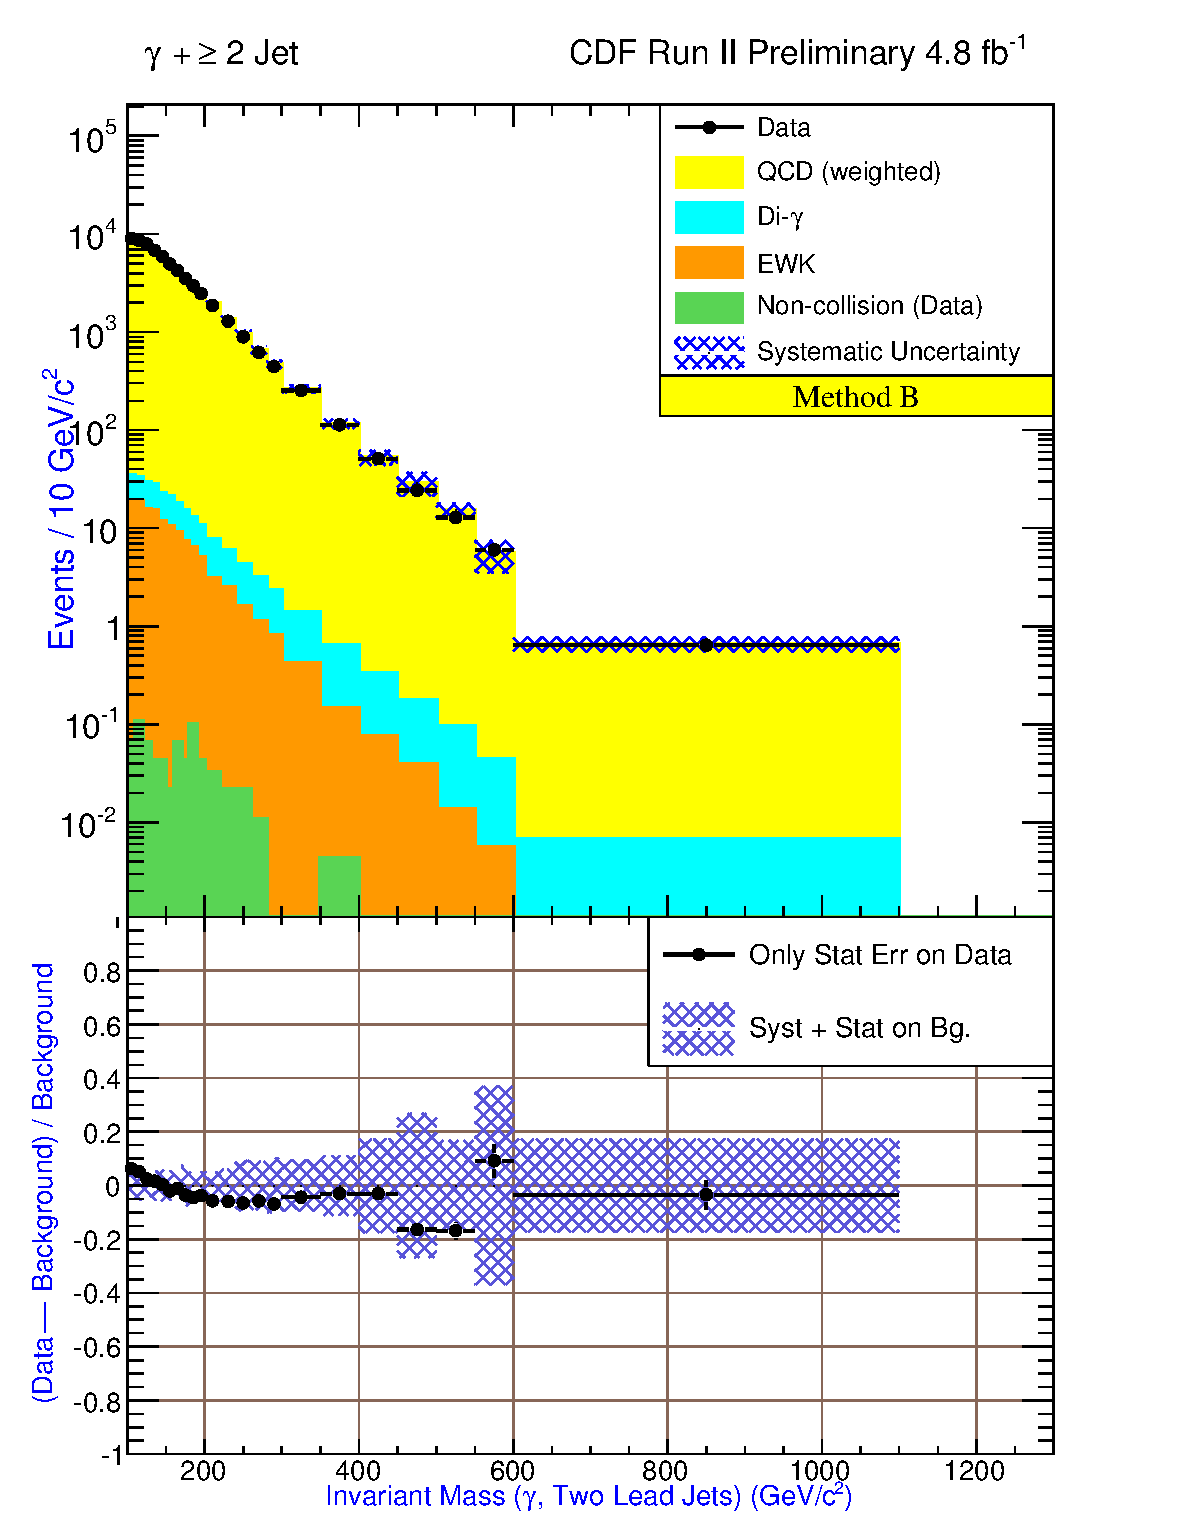
\includegraphics[keepaspectratio=true, scale=\resultsHistScale]{G30Jets_MtdB_plot2_InvMass_pj1j2.pdf}}
\subfigure[]
{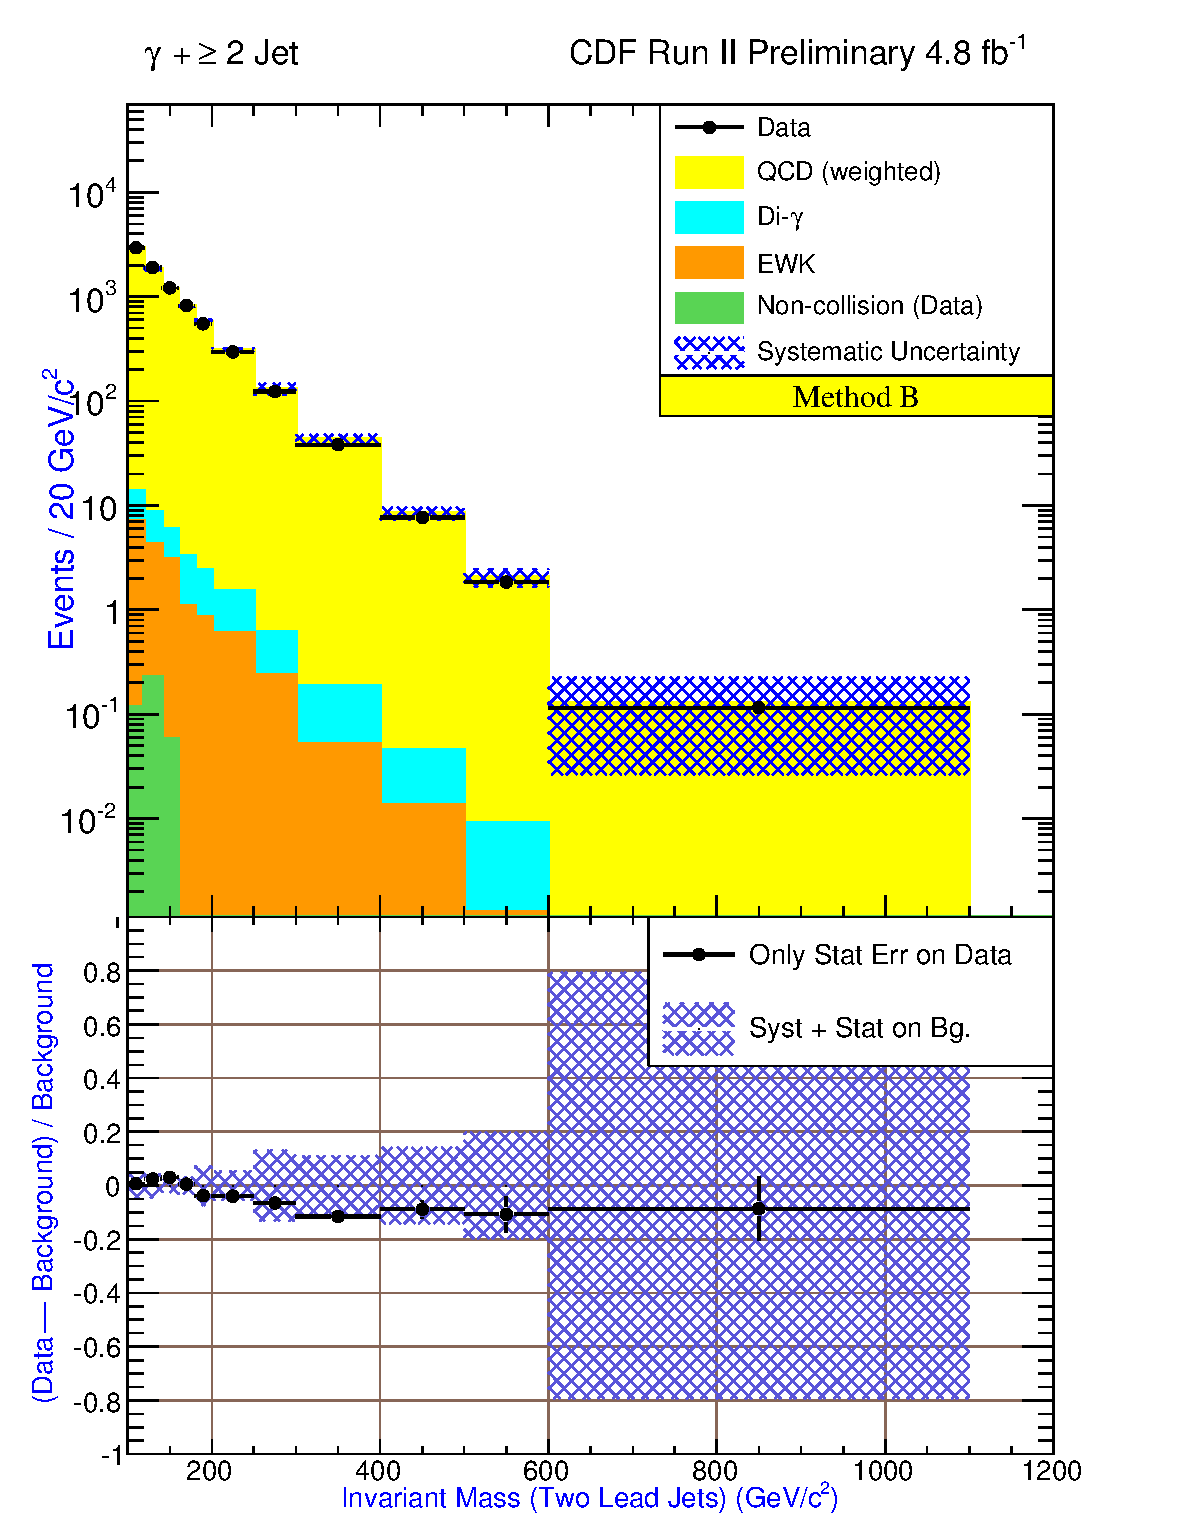
\includegraphics[keepaspectratio=true, scale=\resultsHistScale]{G30Jets_MtdB_plot2_InvMass_j1j2.pdf}}
\caption{Kinematic distributions of \photwojet events using \mbox{Method B}. The beginning of Chapter~\ref{chp:Results} provides a description of the elements in these distributions.}
\label{fig:pjMtdBSetThree}
\end{figure*}
\clearpage

\begin{figure*}[h!]
\centering
{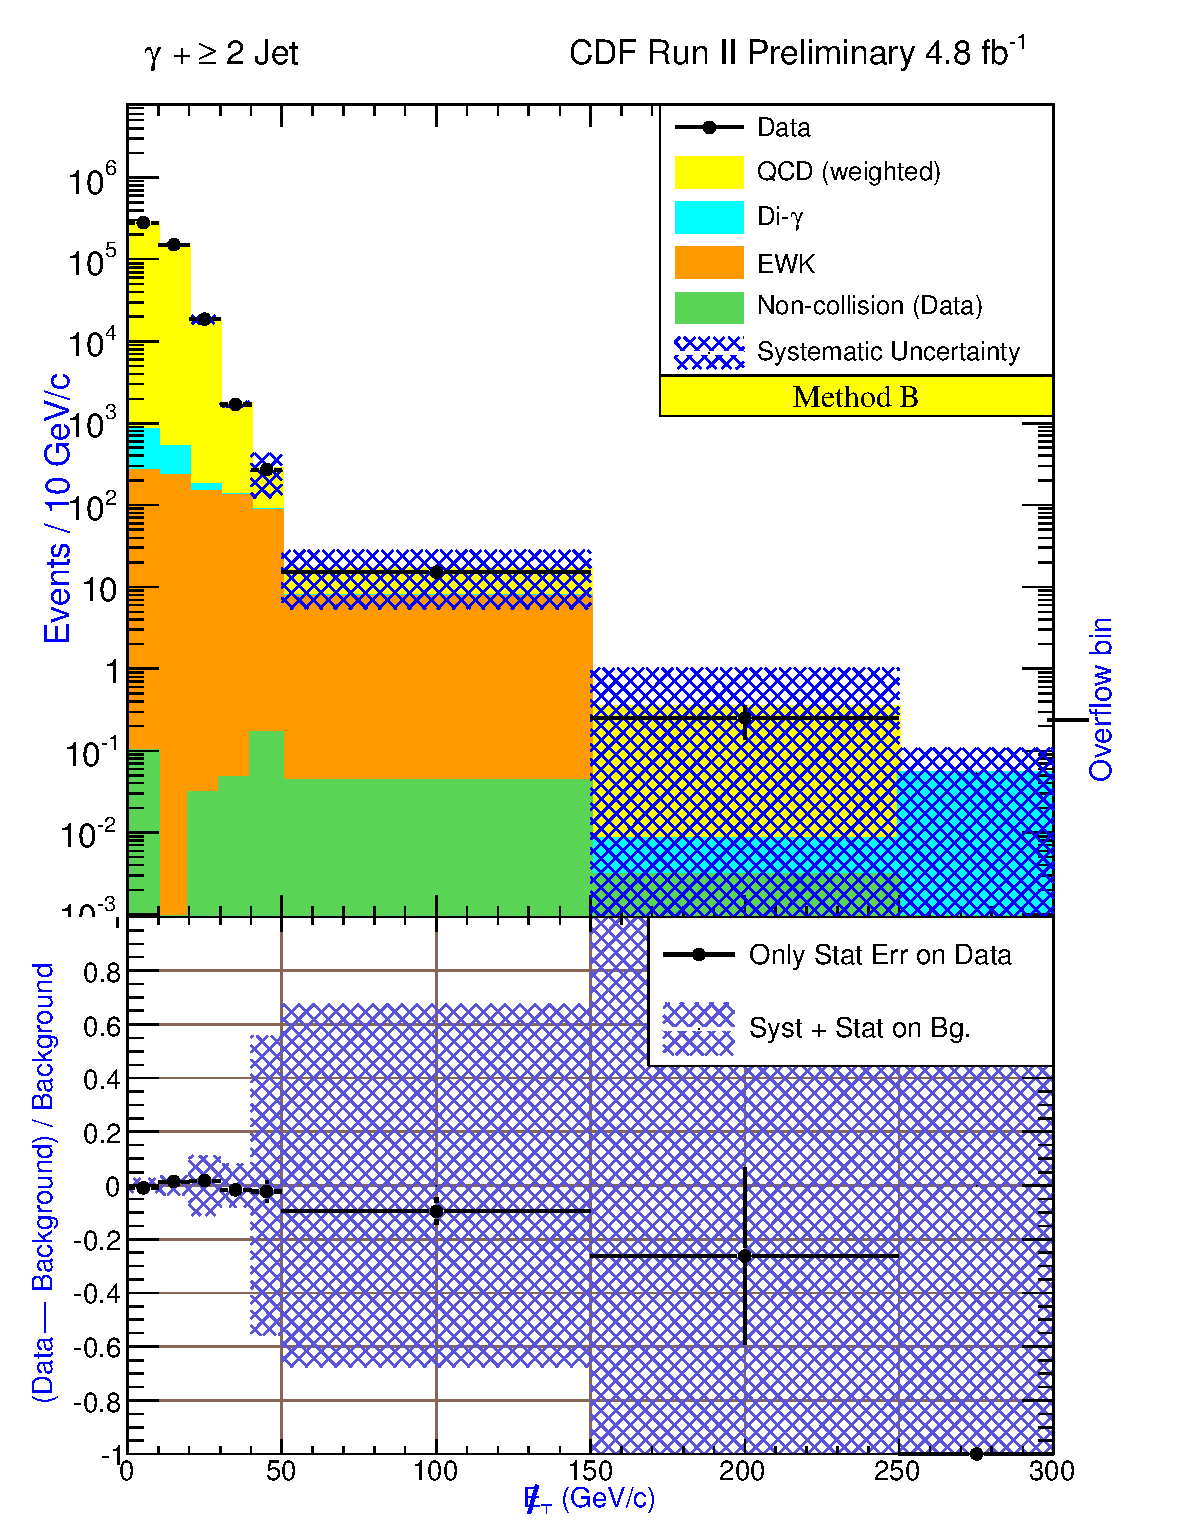
\includegraphics[keepaspectratio=true, scale=0.7]{G30Jets_MtdB_plot2_Met.pdf}}
\caption{Kinematic distributions of \photwojet events using \mbox{Method B}. The beginning of Chapter~\ref{chp:Results} provides a description of the elements in these distributions.}
\label{fig:pjMtdBSetFour}
\end{figure*}
\clearpage

%%%%%%%%%%%%%%%%%%%%%%%%%%%%%%%%%%%% METHOD B: G30 JETS+MET>20

\begin{figure*}[h!]
 \centering
{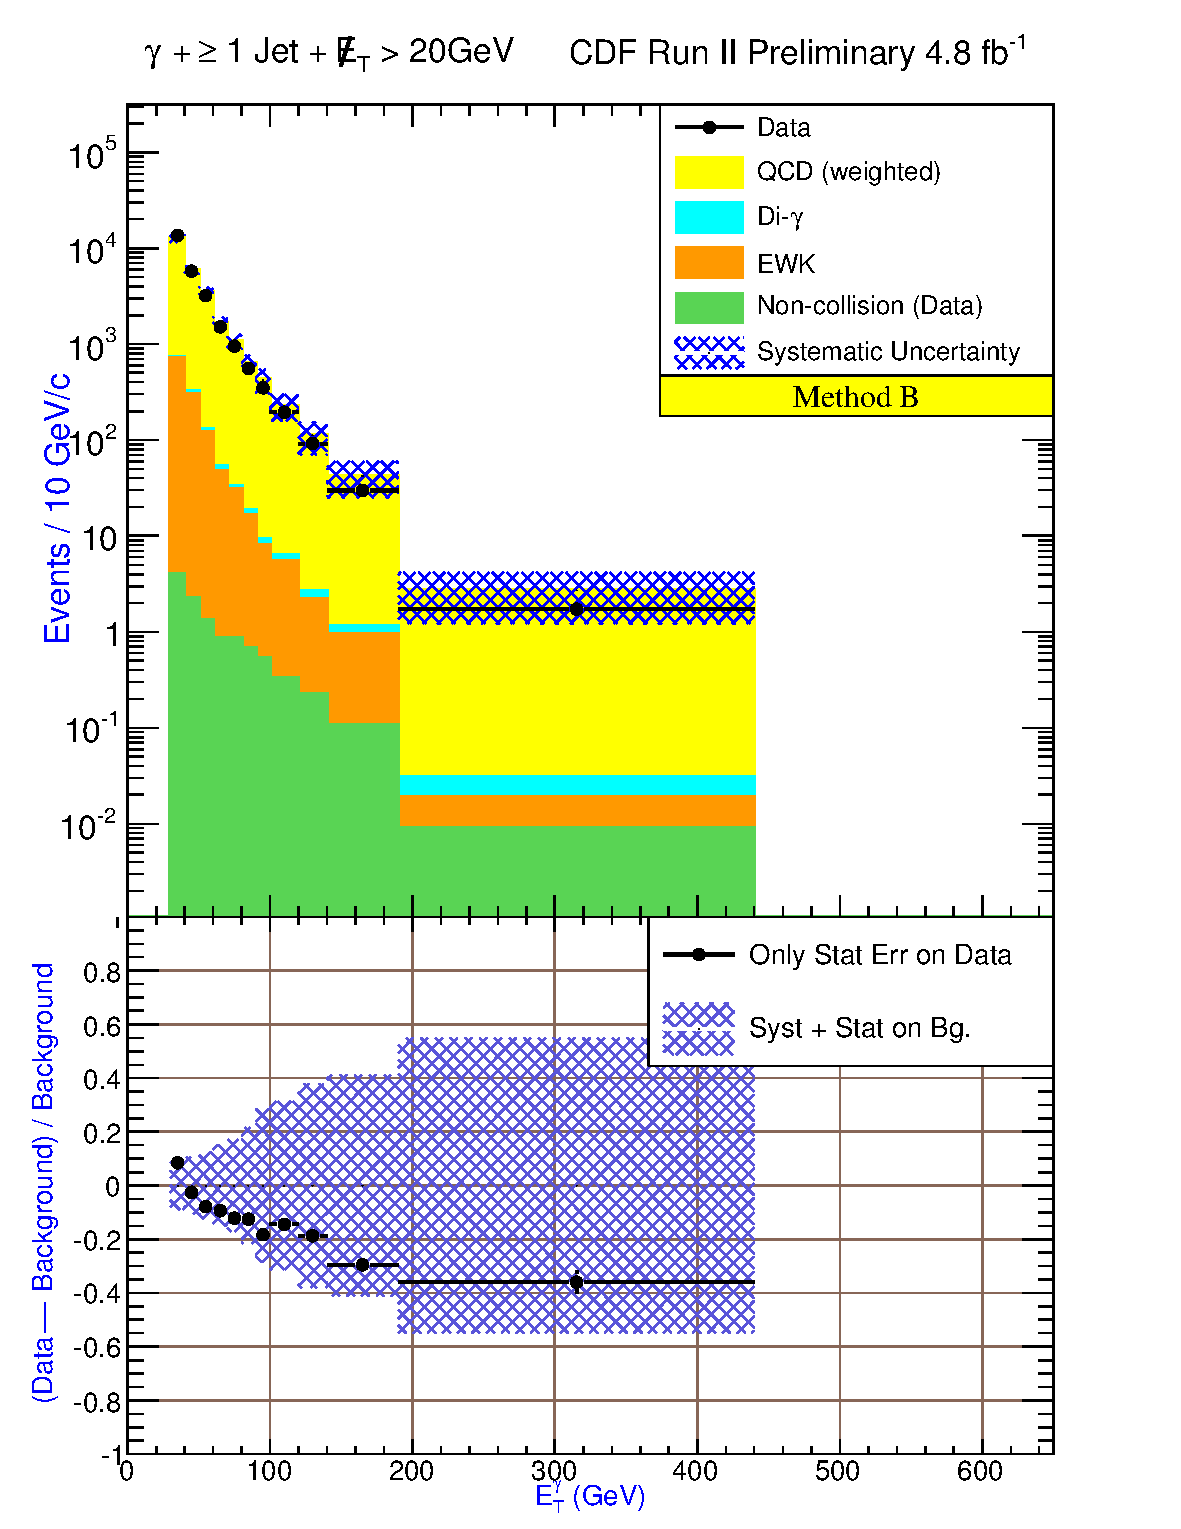
\includegraphics[keepaspectratio=true, scale=\resultsHistScale]{G30JetsMet20_MtdB_plot1_Et_pho.pdf}}
{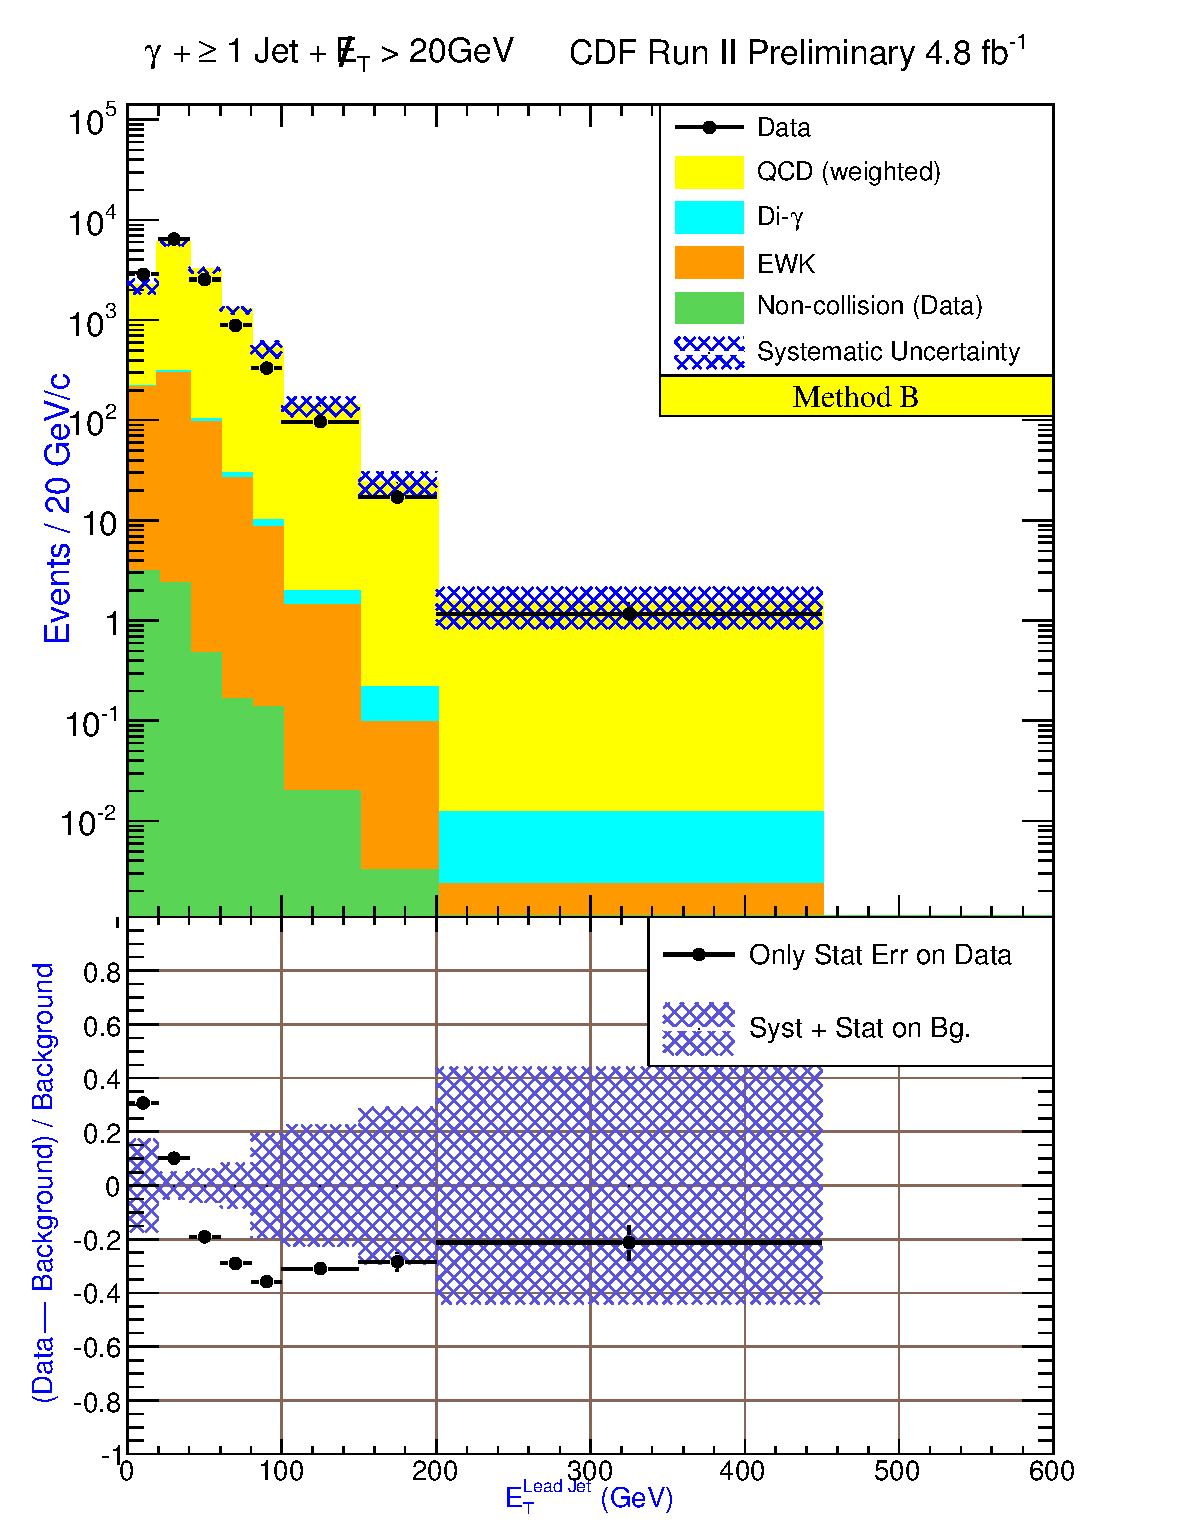
\includegraphics[keepaspectratio=true, scale=\resultsHistScale]{G30JetsMet20_MtdB_plot1_Et_j1.pdf}}
{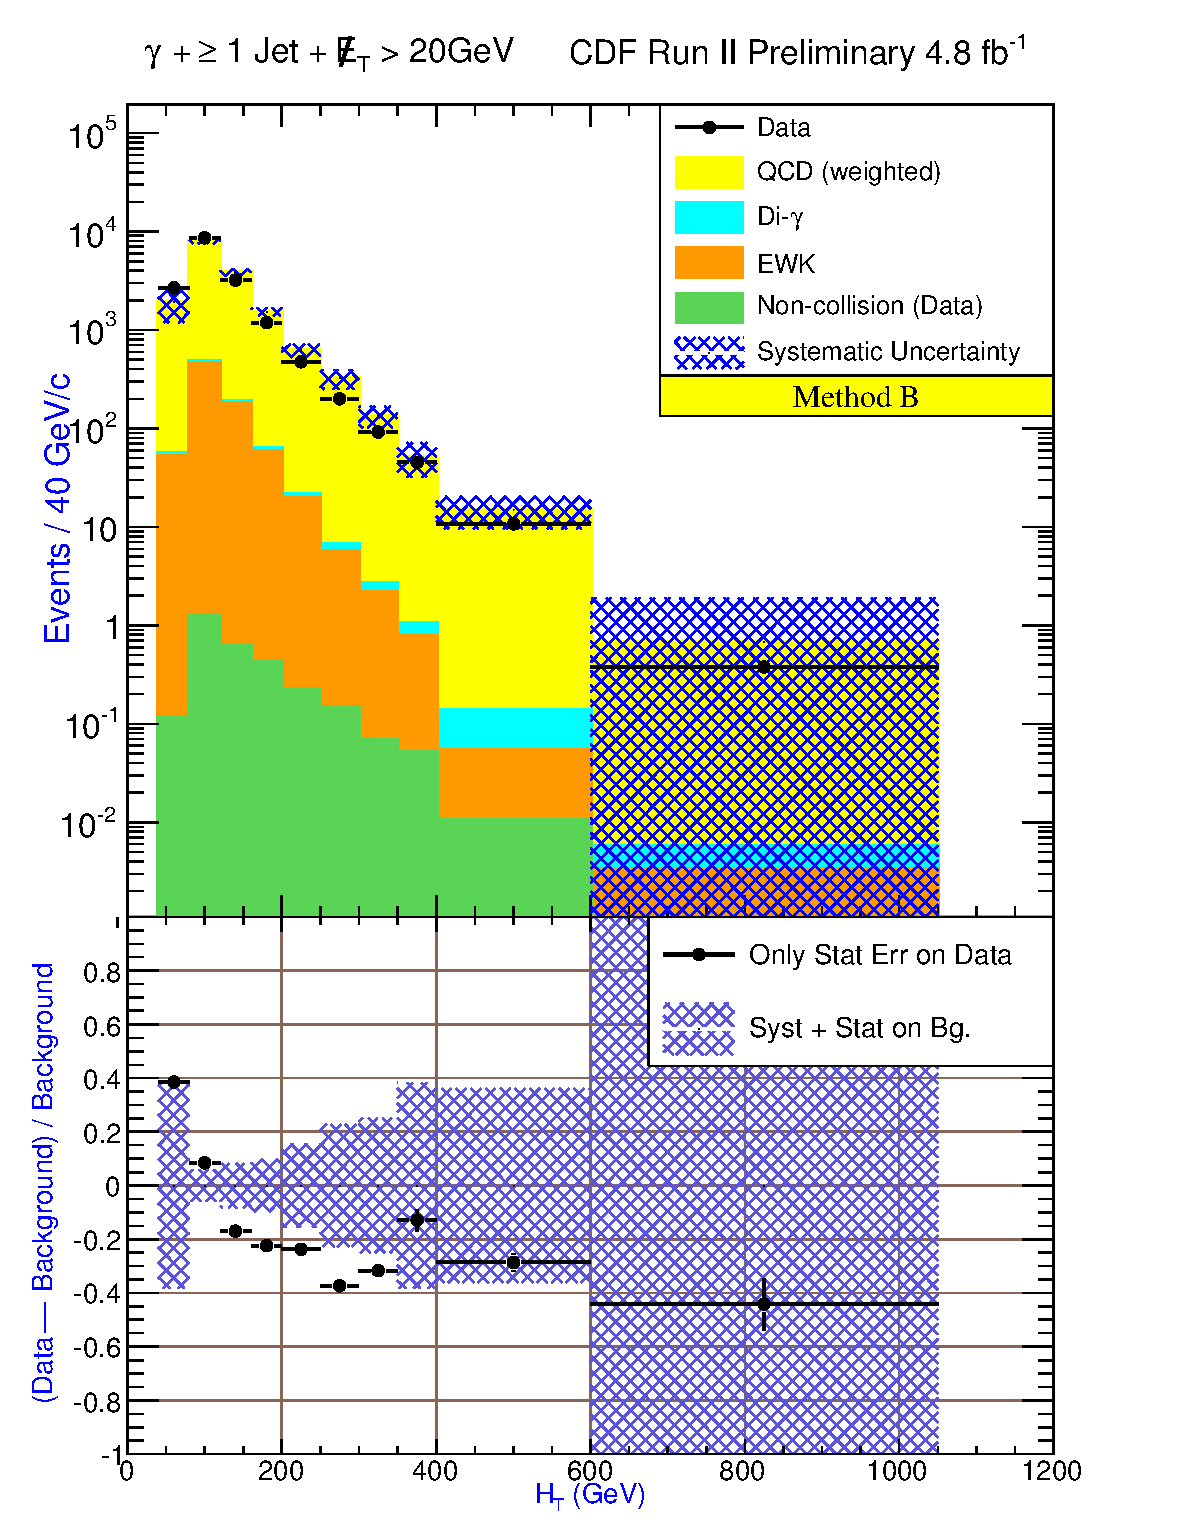
\includegraphics[keepaspectratio=true, scale=\resultsHistScale]{G30JetsMet20_MtdB_plot1_Ht.pdf}}
{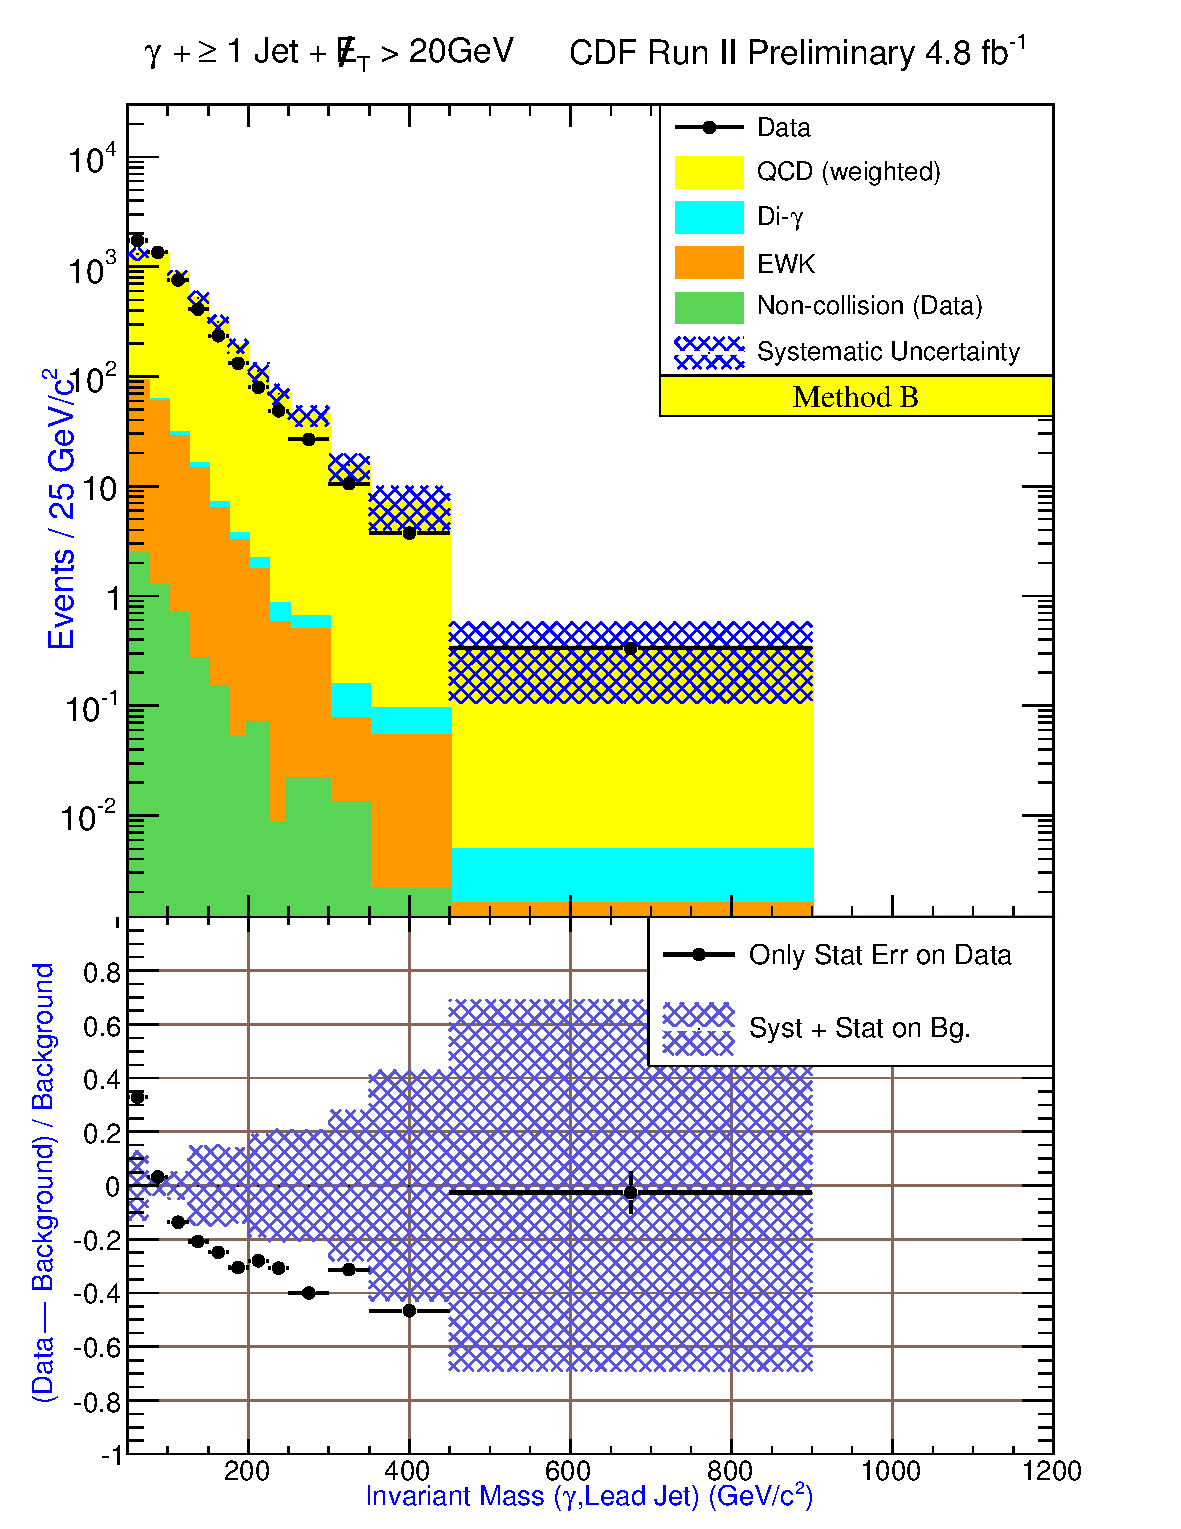
\includegraphics[keepaspectratio=true, scale=\resultsHistScale]{G30JetsMet20_MtdB_plot1_InvMass_pj1.pdf}}
\caption{Kinematic distributions of \phoonejet + \met$>$~20~\etUnits events using \mbox{Method B}. The beginning of Chapter~\ref{chp:Results} provides a description of the elements in these distributions.}
\label{fig:pjmetMtdBSetOne}
\end{figure*}
\clearpage

\begin{figure*}[h!]
\centering
{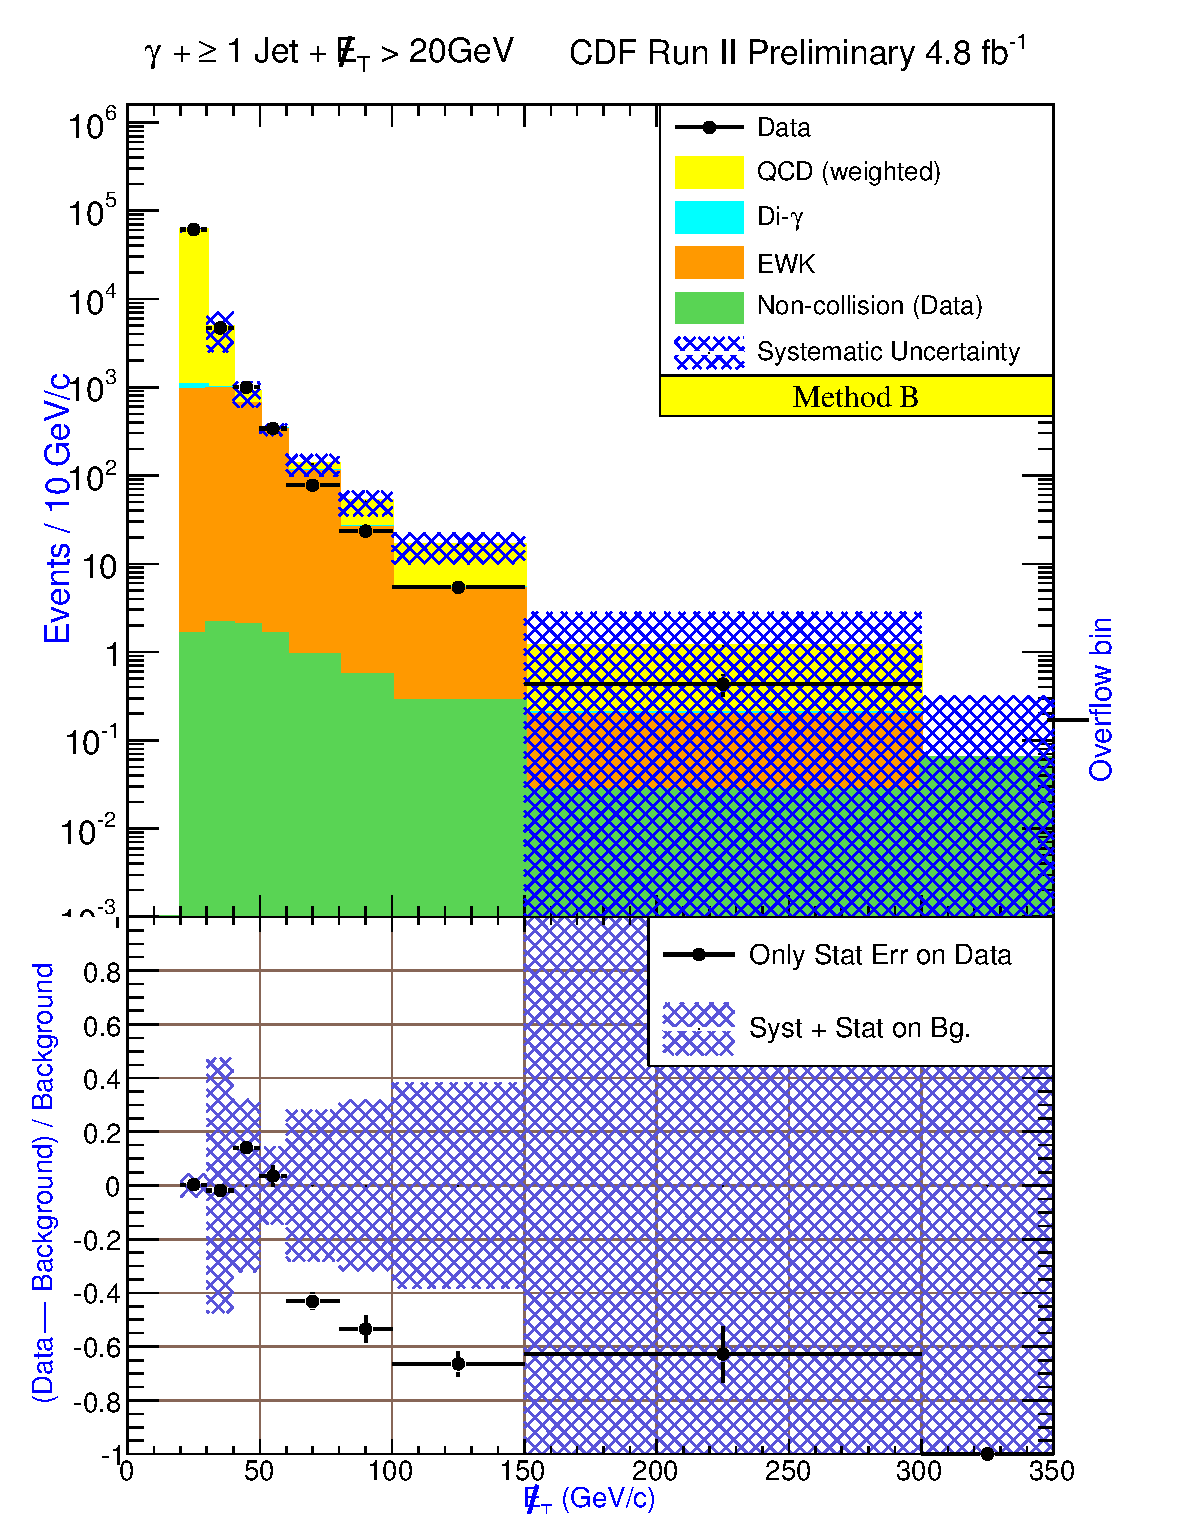
\includegraphics[keepaspectratio=true, scale=\resultsHistScale]{G30JetsMet20_MtdB_plot1_Met.pdf}}
{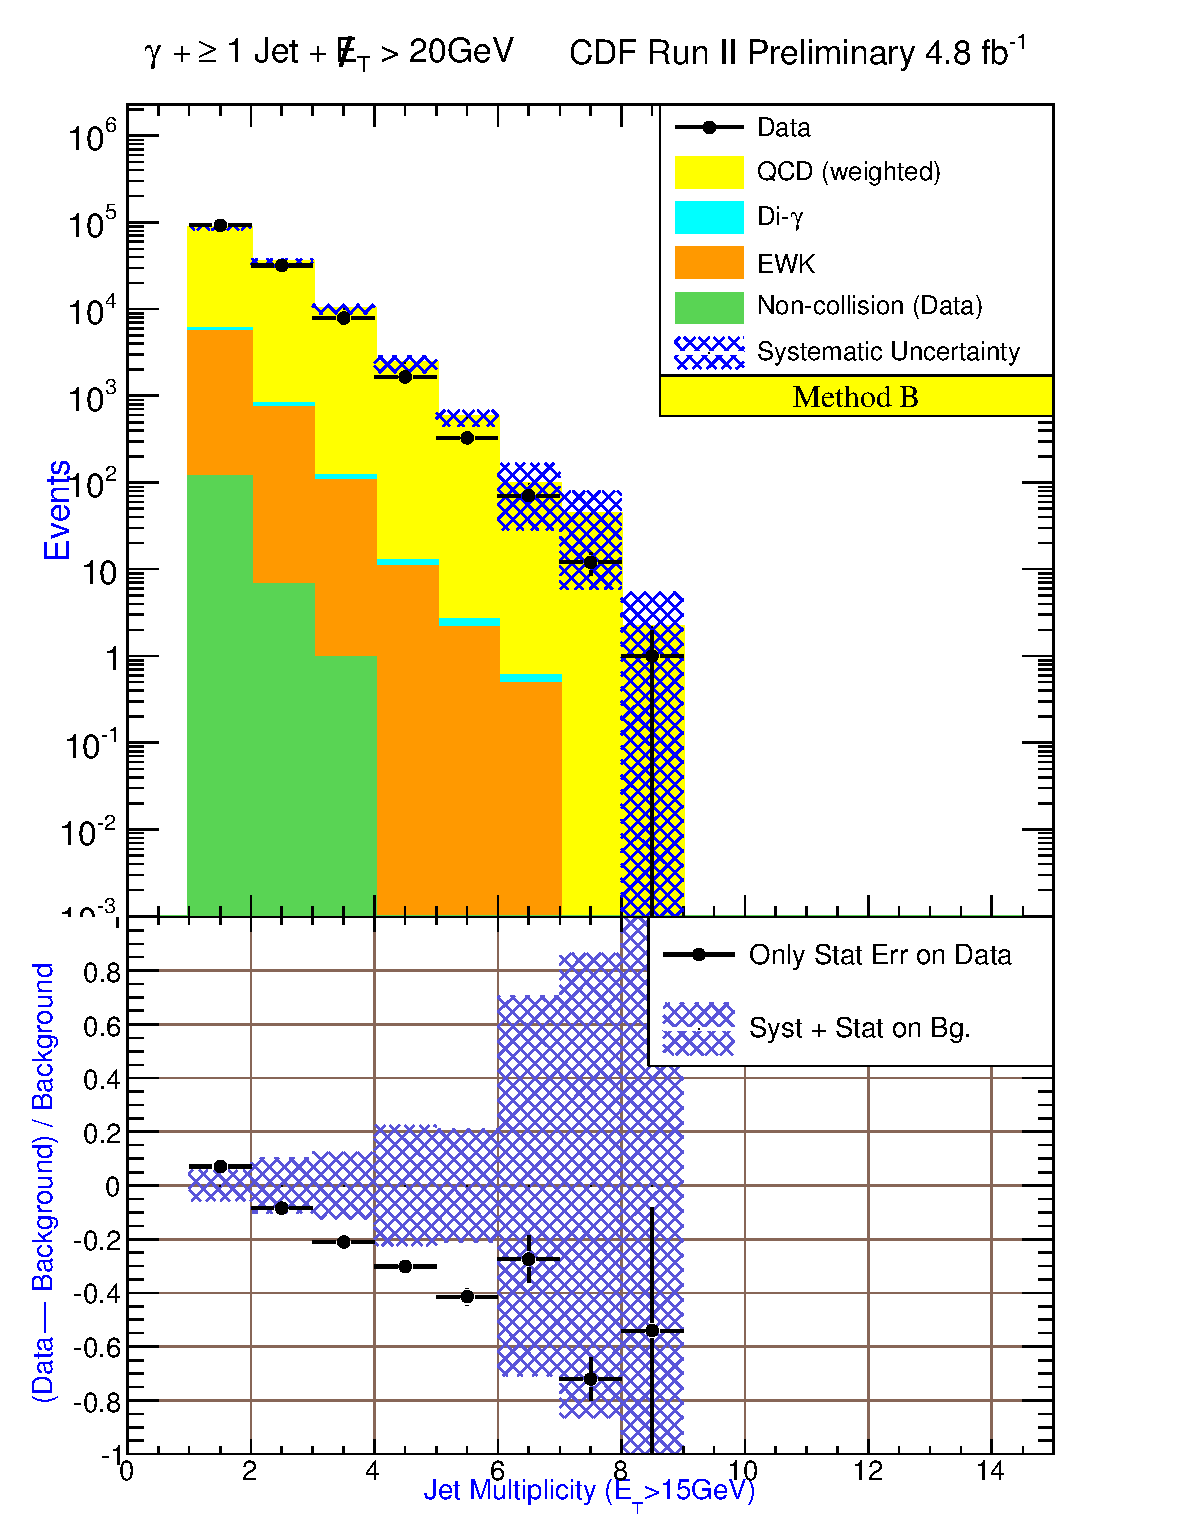
\includegraphics[keepaspectratio=true, scale=\resultsHistScale]{G30JetsMet20_MtdB_plot1_NJet.pdf}}
{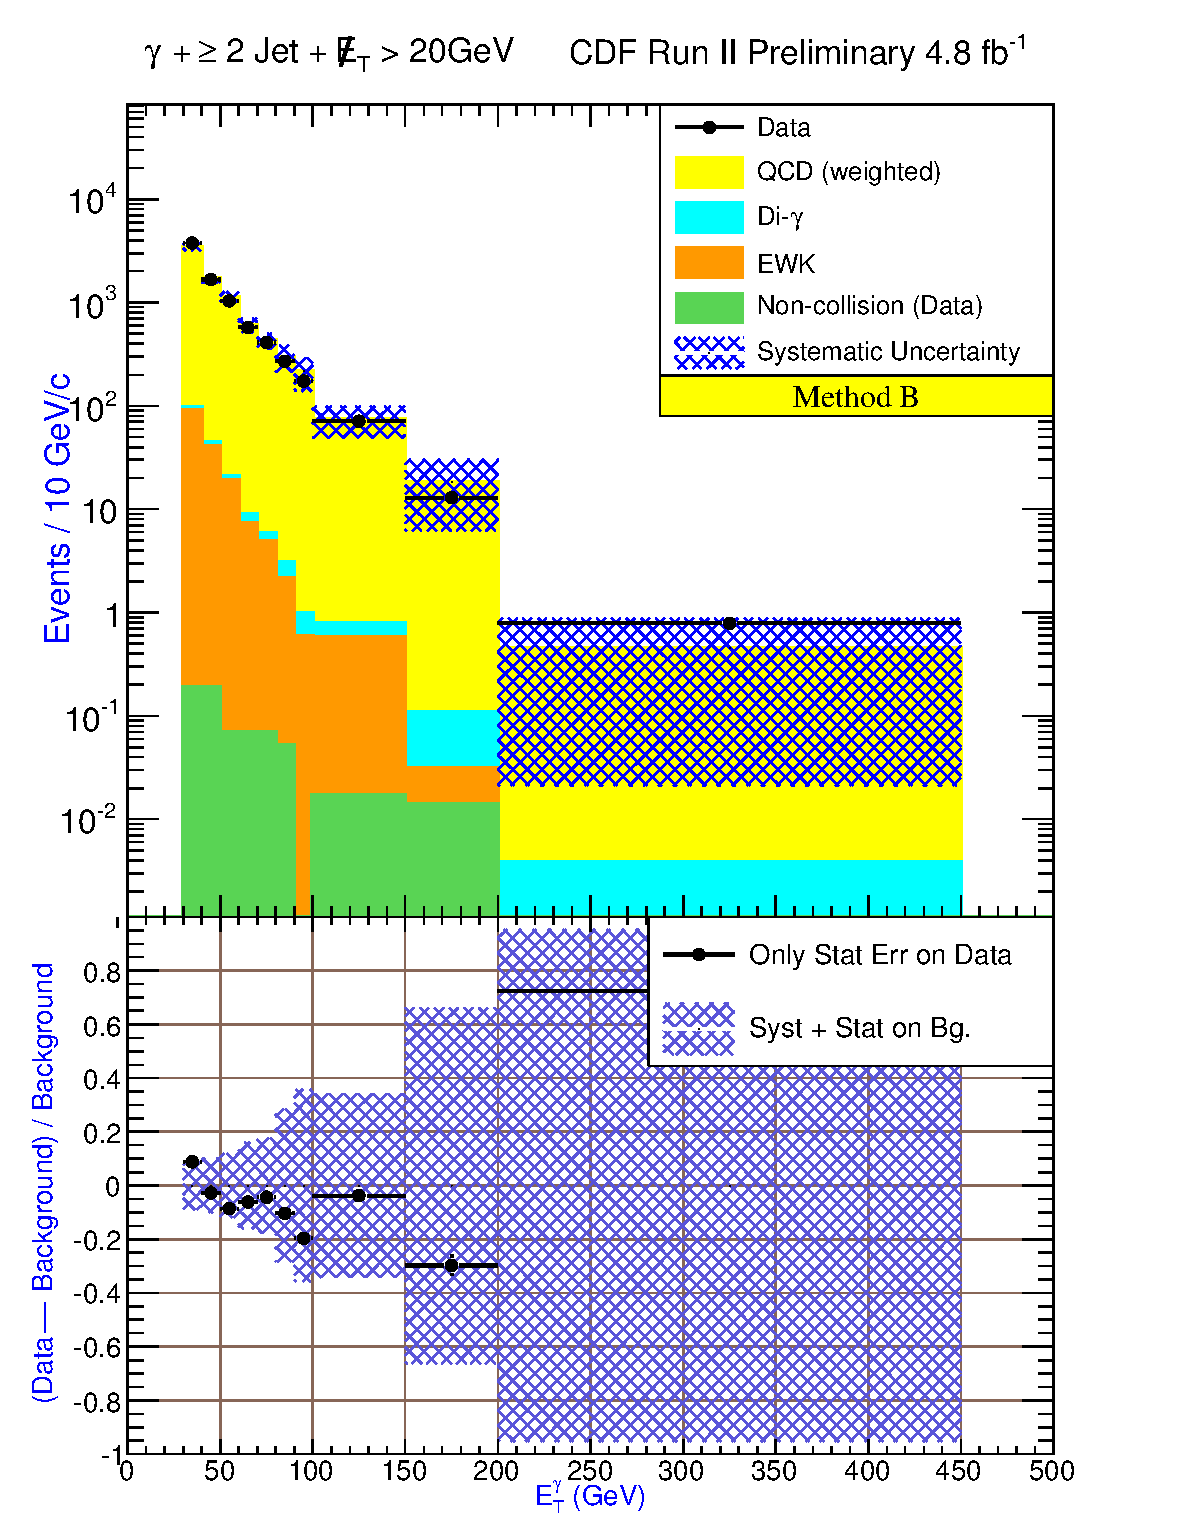
\includegraphics[keepaspectratio=true, scale=\resultsHistScale]{G30JetsMet20_MtdB_plot2_Et_pho.pdf}}
{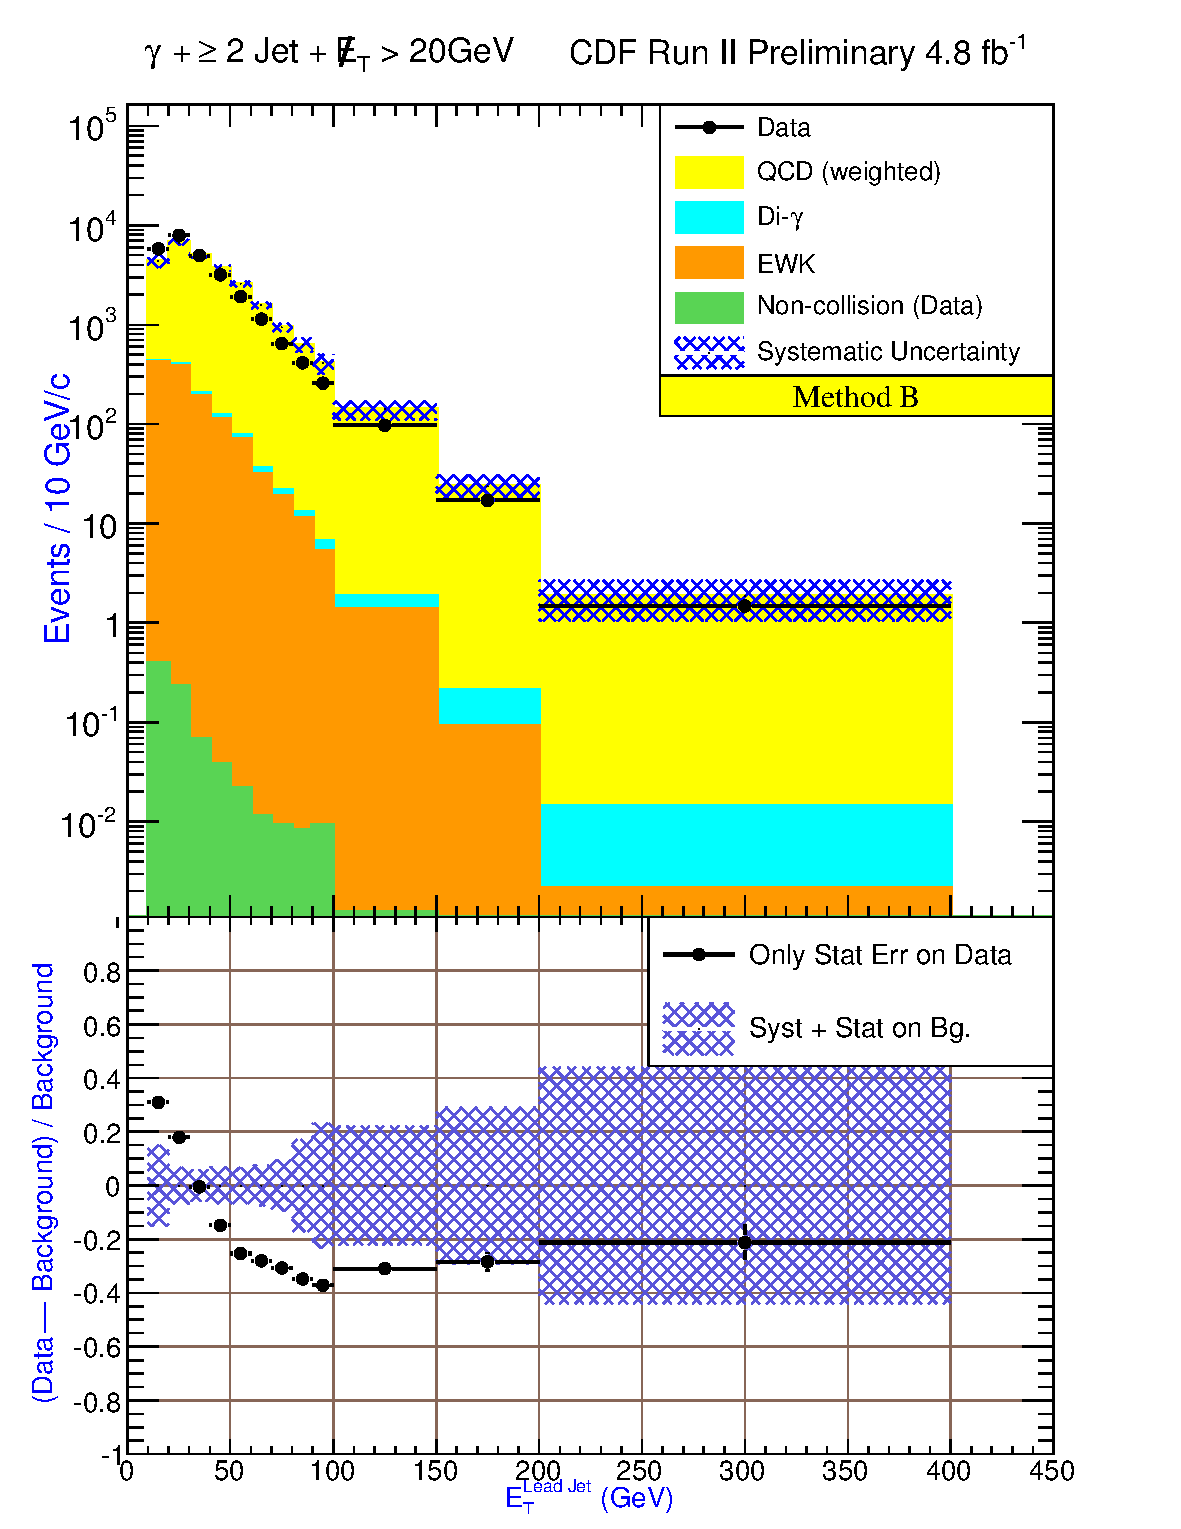
\includegraphics[keepaspectratio=true, scale=\resultsHistScale]{G30JetsMet20_MtdB_plot2_Et_j1.pdf}}
\caption{Kinematic distributions of \phoonejet + \met$>$~20~\etUnits and \photwojet + \met$>$~20~\etUnits events using \mbox{Method B}. The beginning of Chapter~\ref{chp:Results} provides a description of the elements in these distributions.}
\label{fig:pjmetMtdBSetTwo}
\end{figure*}
\clearpage

\begin{figure*}[h!]
\centering
{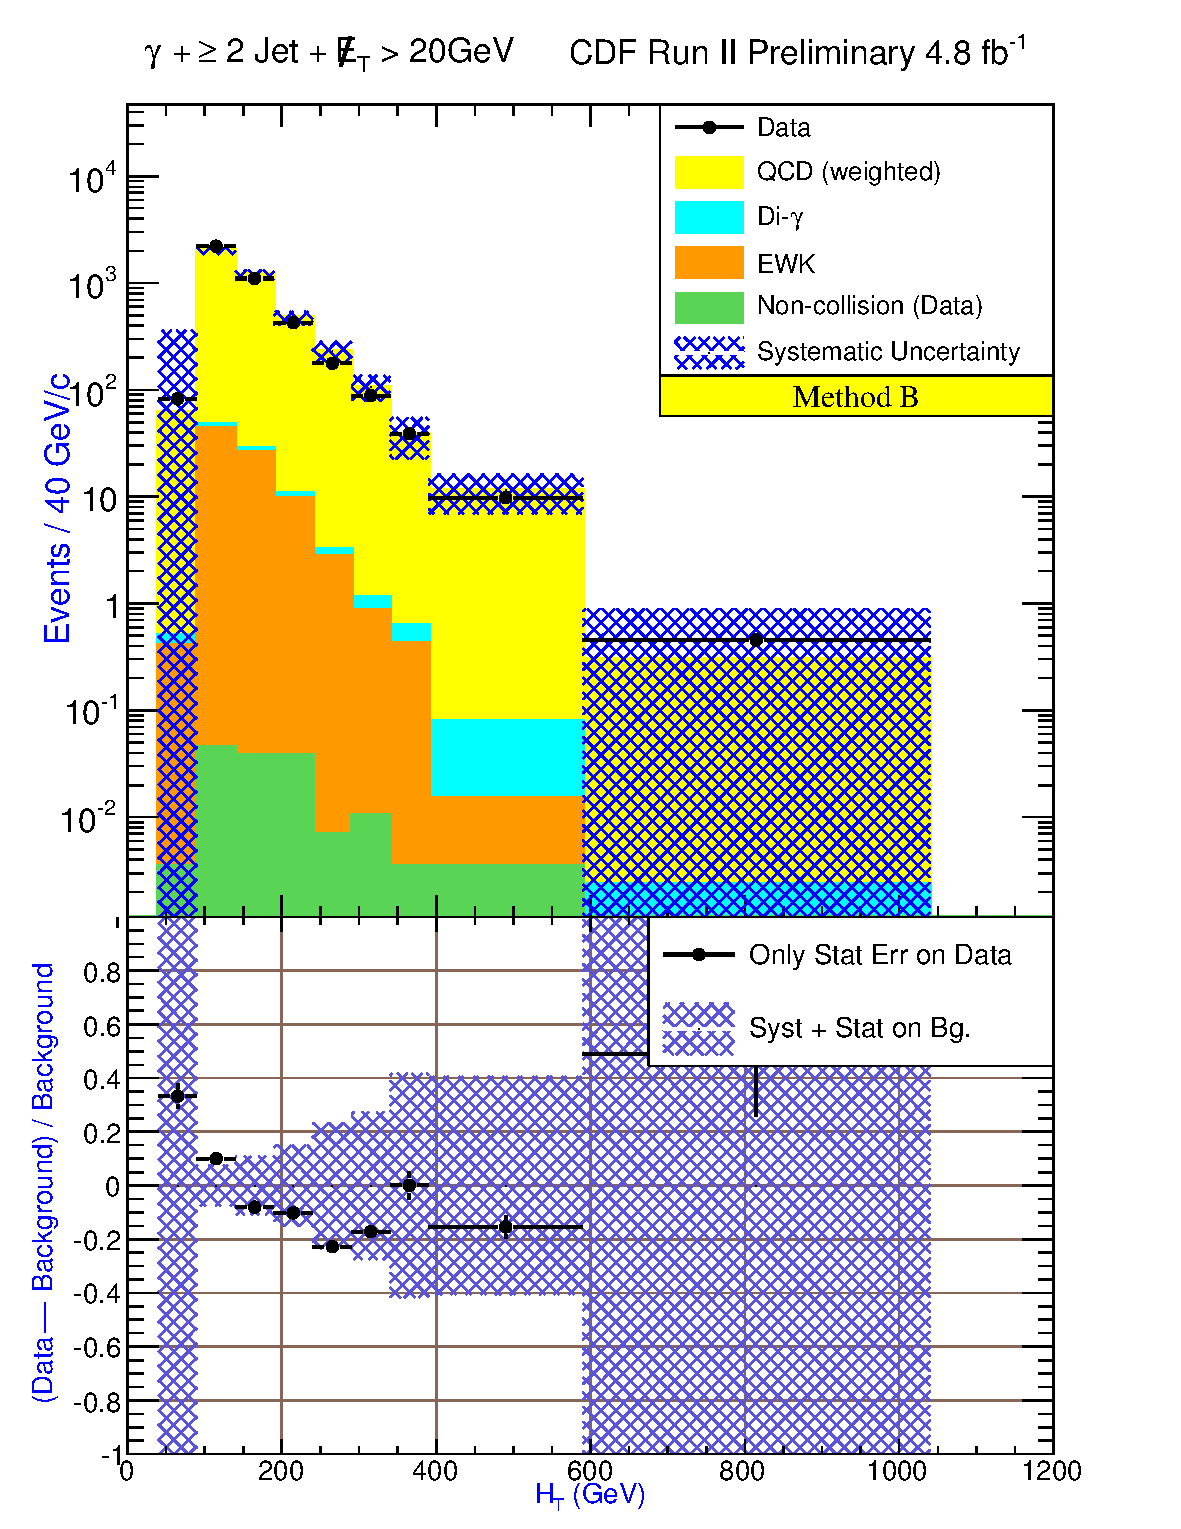
\includegraphics[keepaspectratio=true, scale=\resultsHistScale]{G30JetsMet20_MtdB_plot2_Ht.pdf}}
{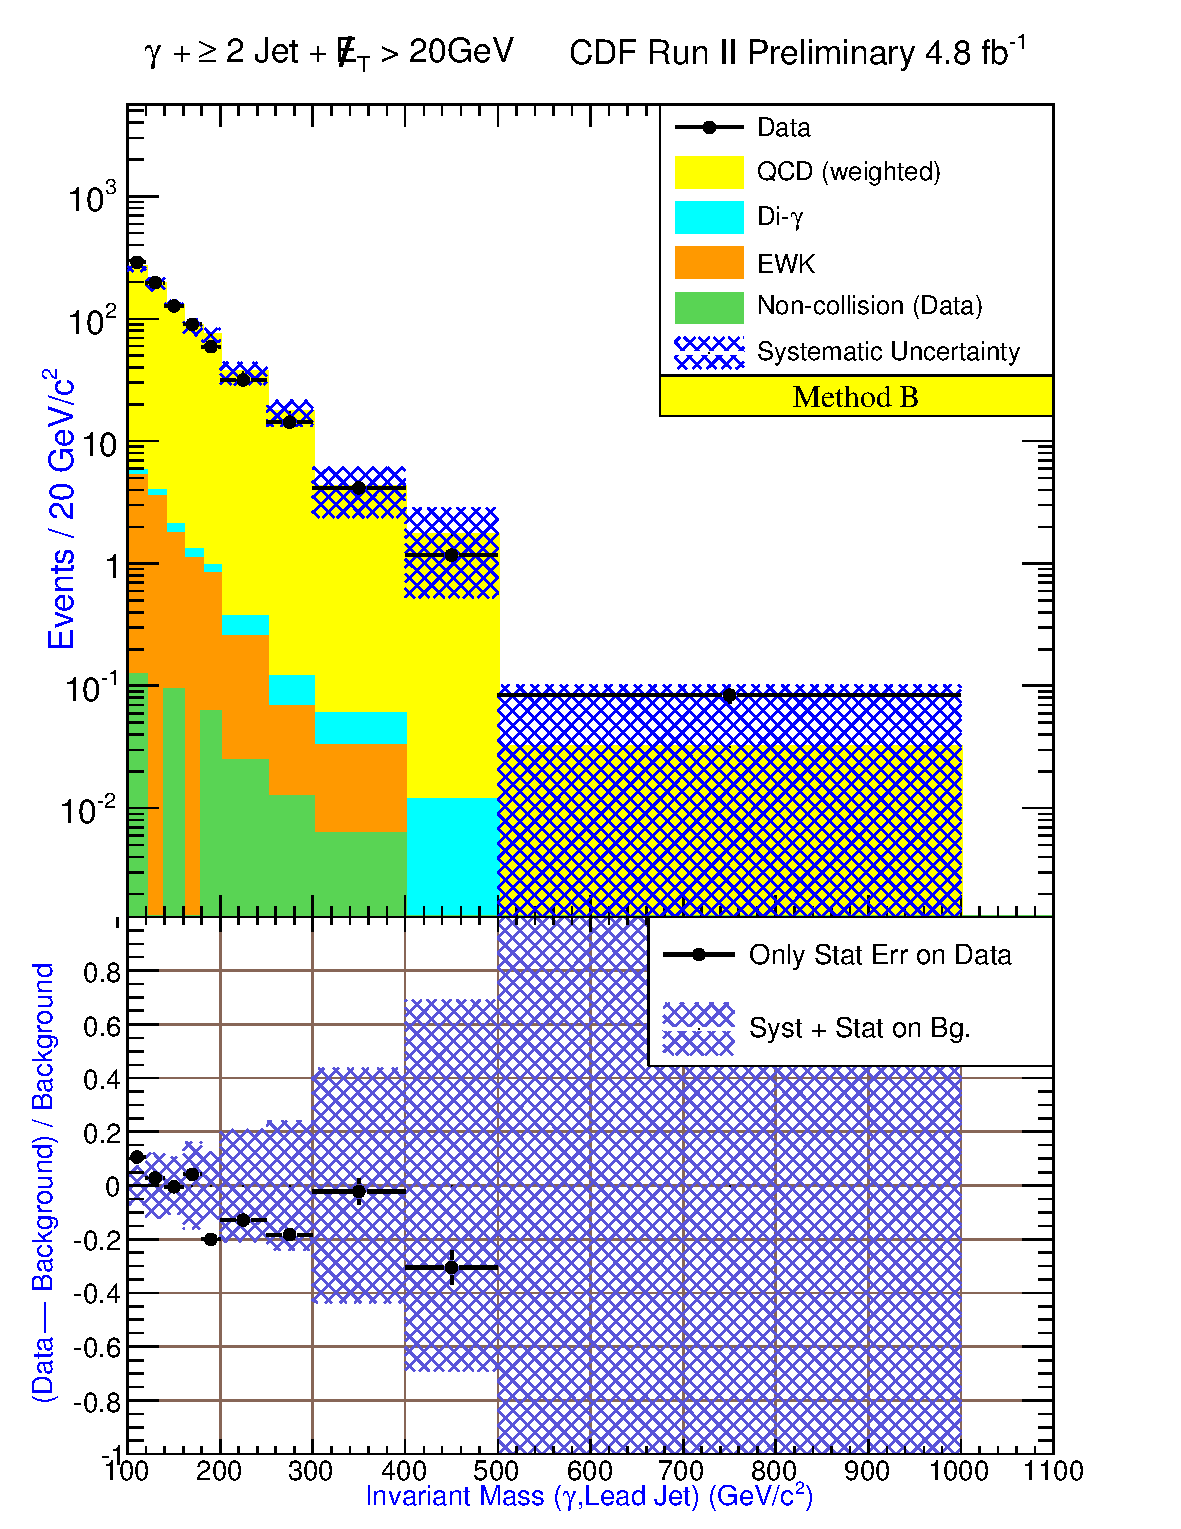
\includegraphics[keepaspectratio=true, scale=\resultsHistScale]{G30JetsMet20_MtdB_plot2_InvMass_pj1.pdf}}
{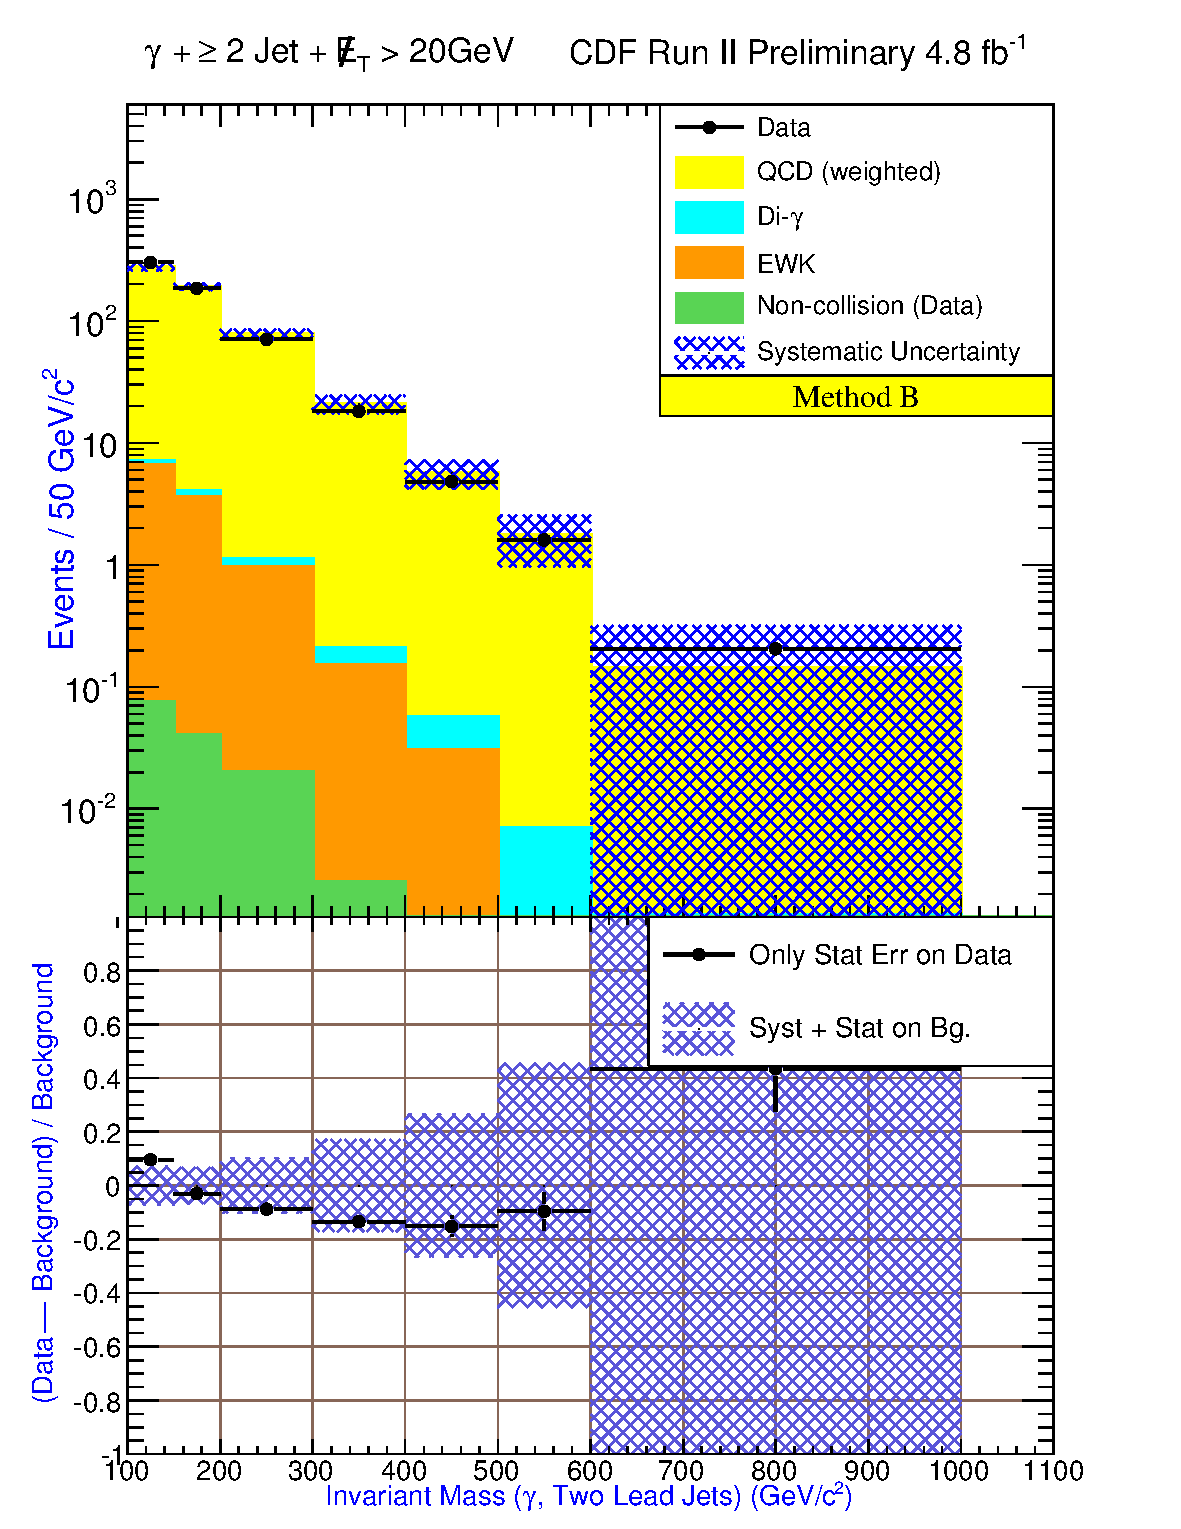
\includegraphics[keepaspectratio=true, scale=\resultsHistScale]{G30JetsMet20_MtdB_plot2_InvMass_pj1j2.pdf}}
{\includegraphics[keepaspectratio=true, scale=\resultsHistScale]{G30JetsMet20_MtdB_plot2_InvMass_j1j2.pdf}}
\caption{Kinematic distributions of \photwojet + \met$>$~20~\etUnits events using \mbox{Method B}. The beginning of Chapter~\ref{chp:Results} provides a description of the elements in these distributions.}
\label{fig:pjmetMtdBSetThree}
\end{figure*}
\clearpage

\begin{figure*}[h!]
\centering
{\includegraphics[keepaspectratio=true, scale=0.7]{G30JetsMet20_MtdB_plot2_Met.pdf}}
\caption{Kinematic distributions of \photwojet + \met$>$~20~\etUnits events using \mbox{Method B}. The beginning of Chapter~\ref{chp:Results} provides a description of the elements in these distributions.}
\label{fig:pjmetMtdBSetFour}
\end{figure*}



\clearpage
\section{Search for Resonance Decay}
As described in the previous section, the mass distributions of the photon and leading jet, photon and two leading jets, and two leading jets in all subsamples are well understood. These measurements are sensitive to contributions of events beyond the SM expectation, which may show up as an excess that indicates a new heavy particle decaying into a photon and jets.

The invariant masses of final-state decay products are searched for a resonance (bump) assuming a null hypothesis. Under a null hypothesis, the assumption is there is no resonance production, which means there should be no significant deviation of data in any region of the mass distribution compared to any other region.

A $\chi^{2}$ statistical test if performed and it is defined as follows:
\begin{equation}
 \chi^{2} = \sum \frac{({\cal O}_{k} - E_{k})^{2}}{\sqrt{E_{k}}}.
 \label{eqa:chi2Stat}
\end{equation}
For a given bin $k$, ${\cal O}_{k}$ is the number of observed data events and $E_{k}$ is the expected number of events. The idea is that the number of data events per bin (${\cal O}_{k}$), should have an average value of $E_{k}$ and would be expected to fluctuate around $E_{k}$ with a standard deviation of order $\sqrt{E_{k}}$. If $\chi^{2}=0$, the agreement between the observed and the expected distribution is perfect, meaning for all bins $k$, ${\cal O}_{k}=E_{k}$. In general, if $\chi^{2}\leq n$ where $n$ is the number of bins, the observed and expected distributions agree reasonably well and no bump can be claimed. If $\chi^{2}>>n$, the observed and the expected distributions differ significantly and a possible bump exists.

Figures \ref{fig:MassFit_pj1_pj}--\ref{fig:MassFit_pj2met_j1j2} shows the fits to mass distributions of the photon and leading jet, photon and two leading jets, and two leading jets for the inclusive photon + jets sample and the photon + jets + \metg{20} sample. The data are binned in variable-bin sizes to improve statistics. The data are shown with black circles, and black lines show the statistical uncertainty. The blue curve is the fitted line. The bottom plot shows the deviation of data points from the fit.


\begin{figure}[htb!]
\centering
\includegraphics[scale=\resultsMassFitScale,keepaspectratio=true]{gjets_pj1_pj1MassFit.pdf}
\caption{Invariant mass distribution of the photon and the leading jet in $\gamma$~+ $\geq$1 jet events.}
\label{fig:MassFit_pj1_pj}
\end{figure}

 \begin{figure}[htb!]
\centering
\includegraphics[scale=\resultsMassFitScale,keepaspectratio=true]{gjets_pj2_pj1MassFit.pdf}
\caption{Invariant mass distribution of the photon and the leading jet in $\gamma$~+ $\geq$2 jets events.}
\label{fig:MassFit_pj2_pj}
\end{figure}

\begin{figure}[htb!]
\centering
\includegraphics[scale=\resultsMassFitScale,keepaspectratio=true]{gjets_pj2_pj1j2MassFit.pdf}
\caption{Invariant mass distribution of the photon and the two leading jet in $\gamma$~+ $\geq$2 jets events.}
\label{fig:MassFit_pj2_pj1j2}
\end{figure}

\begin{figure}[htb!]
\centering
\includegraphics[scale=\resultsMassFitScale,keepaspectratio=true]{gjets_pj2_j1j2MassFit.pdf}
\caption[Invariant mass distribution of the two leading jets in $\gamma$~+ $\geq$2 \mbox{jets } events.]{Invariant mass distribution of the two leading jets in $\gamma$~+ $\geq$2 jets events.}
\label{fig:MassFit_pj2_j1j2}
\end{figure}


\begin{figure}[htb!]
\centering
\includegraphics[scale=\resultsMassFitScale,keepaspectratio=true]{gjetsmet_pj1_pj1MassFit.pdf}
\caption{Invariant mass distribution of the photon and the leading jet in $\gamma$~+ $\geq$1 jet + \metg{20} events.}
\label{fig:MassFit_pj1met_pj}
\end{figure}

 \begin{figure}[htb!]
\centering
\includegraphics[scale=\resultsMassFitScale,keepaspectratio=true]{gjetsmet_pj2_pj1MassFit.pdf}
\caption{Invariant mass distribution of the photon and the leading jet in $\gamma$~+ $\geq$2 jets + \metg{20} events.}
\label{fig:MassFit_pj2met_pj}
\end{figure}

\begin{figure}[htb!]
\centering
\includegraphics[scale=\resultsMassFitScale,keepaspectratio=true]{gjetsmet_pj2_pj1j2MassFit.pdf}
\caption{Invariant mass distribution of the photon and the leading jet in $\gamma$~+ $\geq$2 jets + \metg{20} events.}
\label{fig:MassFit_pj2met_pj1j2}
\end{figure}

\begin{figure}[htb!]
\centering
\includegraphics[scale=\resultsMassFitScale,keepaspectratio=true]{gjetsmet_pj2_j1j2MassFit.pdf}
\caption{Invariant mass distribution of the two leading jets in $\gamma$~+ $\geq$2 jets + \metg{20} events.}
\label{fig:MassFit_pj2met_j1j2}
\end{figure}


